% Options for packages loaded elsewhere
\PassOptionsToPackage{unicode}{hyperref}
\PassOptionsToPackage{hyphens}{url}
%
\documentclass[
]{article}
\usepackage{amsmath,amssymb}
\usepackage{lmodern}
\usepackage{ifxetex,ifluatex}
\ifnum 0\ifxetex 1\fi\ifluatex 1\fi=0 % if pdftex
  \usepackage[T1]{fontenc}
  \usepackage[utf8]{inputenc}
  \usepackage{textcomp} % provide euro and other symbols
\else % if luatex or xetex
  \usepackage{unicode-math}
  \defaultfontfeatures{Scale=MatchLowercase}
  \defaultfontfeatures[\rmfamily]{Ligatures=TeX,Scale=1}
\fi
% Use upquote if available, for straight quotes in verbatim environments
\IfFileExists{upquote.sty}{\usepackage{upquote}}{}
\IfFileExists{microtype.sty}{% use microtype if available
  \usepackage[]{microtype}
  \UseMicrotypeSet[protrusion]{basicmath} % disable protrusion for tt fonts
}{}
\makeatletter
\@ifundefined{KOMAClassName}{% if non-KOMA class
  \IfFileExists{parskip.sty}{%
    \usepackage{parskip}
  }{% else
    \setlength{\parindent}{0pt}
    \setlength{\parskip}{6pt plus 2pt minus 1pt}}
}{% if KOMA class
  \KOMAoptions{parskip=half}}
\makeatother
\usepackage{xcolor}
\IfFileExists{xurl.sty}{\usepackage{xurl}}{} % add URL line breaks if available
\IfFileExists{bookmark.sty}{\usepackage{bookmark}}{\usepackage{hyperref}}
\hypersetup{
  pdftitle={Tutorial R e RStudio},
  hidelinks,
  pdfcreator={LaTeX via pandoc}}
\urlstyle{same} % disable monospaced font for URLs
\usepackage[margin=1in]{geometry}
\usepackage{color}
\usepackage{fancyvrb}
\newcommand{\VerbBar}{|}
\newcommand{\VERB}{\Verb[commandchars=\\\{\}]}
\DefineVerbatimEnvironment{Highlighting}{Verbatim}{commandchars=\\\{\}}
% Add ',fontsize=\small' for more characters per line
\usepackage{framed}
\definecolor{shadecolor}{RGB}{248,248,248}
\newenvironment{Shaded}{\begin{snugshade}}{\end{snugshade}}
\newcommand{\AlertTok}[1]{\textcolor[rgb]{0.94,0.16,0.16}{#1}}
\newcommand{\AnnotationTok}[1]{\textcolor[rgb]{0.56,0.35,0.01}{\textbf{\textit{#1}}}}
\newcommand{\AttributeTok}[1]{\textcolor[rgb]{0.77,0.63,0.00}{#1}}
\newcommand{\BaseNTok}[1]{\textcolor[rgb]{0.00,0.00,0.81}{#1}}
\newcommand{\BuiltInTok}[1]{#1}
\newcommand{\CharTok}[1]{\textcolor[rgb]{0.31,0.60,0.02}{#1}}
\newcommand{\CommentTok}[1]{\textcolor[rgb]{0.56,0.35,0.01}{\textit{#1}}}
\newcommand{\CommentVarTok}[1]{\textcolor[rgb]{0.56,0.35,0.01}{\textbf{\textit{#1}}}}
\newcommand{\ConstantTok}[1]{\textcolor[rgb]{0.00,0.00,0.00}{#1}}
\newcommand{\ControlFlowTok}[1]{\textcolor[rgb]{0.13,0.29,0.53}{\textbf{#1}}}
\newcommand{\DataTypeTok}[1]{\textcolor[rgb]{0.13,0.29,0.53}{#1}}
\newcommand{\DecValTok}[1]{\textcolor[rgb]{0.00,0.00,0.81}{#1}}
\newcommand{\DocumentationTok}[1]{\textcolor[rgb]{0.56,0.35,0.01}{\textbf{\textit{#1}}}}
\newcommand{\ErrorTok}[1]{\textcolor[rgb]{0.64,0.00,0.00}{\textbf{#1}}}
\newcommand{\ExtensionTok}[1]{#1}
\newcommand{\FloatTok}[1]{\textcolor[rgb]{0.00,0.00,0.81}{#1}}
\newcommand{\FunctionTok}[1]{\textcolor[rgb]{0.00,0.00,0.00}{#1}}
\newcommand{\ImportTok}[1]{#1}
\newcommand{\InformationTok}[1]{\textcolor[rgb]{0.56,0.35,0.01}{\textbf{\textit{#1}}}}
\newcommand{\KeywordTok}[1]{\textcolor[rgb]{0.13,0.29,0.53}{\textbf{#1}}}
\newcommand{\NormalTok}[1]{#1}
\newcommand{\OperatorTok}[1]{\textcolor[rgb]{0.81,0.36,0.00}{\textbf{#1}}}
\newcommand{\OtherTok}[1]{\textcolor[rgb]{0.56,0.35,0.01}{#1}}
\newcommand{\PreprocessorTok}[1]{\textcolor[rgb]{0.56,0.35,0.01}{\textit{#1}}}
\newcommand{\RegionMarkerTok}[1]{#1}
\newcommand{\SpecialCharTok}[1]{\textcolor[rgb]{0.00,0.00,0.00}{#1}}
\newcommand{\SpecialStringTok}[1]{\textcolor[rgb]{0.31,0.60,0.02}{#1}}
\newcommand{\StringTok}[1]{\textcolor[rgb]{0.31,0.60,0.02}{#1}}
\newcommand{\VariableTok}[1]{\textcolor[rgb]{0.00,0.00,0.00}{#1}}
\newcommand{\VerbatimStringTok}[1]{\textcolor[rgb]{0.31,0.60,0.02}{#1}}
\newcommand{\WarningTok}[1]{\textcolor[rgb]{0.56,0.35,0.01}{\textbf{\textit{#1}}}}
\usepackage{longtable,booktabs,array}
\usepackage{calc} % for calculating minipage widths
% Correct order of tables after \paragraph or \subparagraph
\usepackage{etoolbox}
\makeatletter
\patchcmd\longtable{\par}{\if@noskipsec\mbox{}\fi\par}{}{}
\makeatother
% Allow footnotes in longtable head/foot
\IfFileExists{footnotehyper.sty}{\usepackage{footnotehyper}}{\usepackage{footnote}}
\makesavenoteenv{longtable}
\usepackage{graphicx}
\makeatletter
\def\maxwidth{\ifdim\Gin@nat@width>\linewidth\linewidth\else\Gin@nat@width\fi}
\def\maxheight{\ifdim\Gin@nat@height>\textheight\textheight\else\Gin@nat@height\fi}
\makeatother
% Scale images if necessary, so that they will not overflow the page
% margins by default, and it is still possible to overwrite the defaults
% using explicit options in \includegraphics[width, height, ...]{}
\setkeys{Gin}{width=\maxwidth,height=\maxheight,keepaspectratio}
% Set default figure placement to htbp
\makeatletter
\def\fps@figure{htbp}
\makeatother
\setlength{\emergencystretch}{3em} % prevent overfull lines
\providecommand{\tightlist}{%
  \setlength{\itemsep}{0pt}\setlength{\parskip}{0pt}}
\setcounter{secnumdepth}{-\maxdimen} % remove section numbering
\usepackage{booktabs}
\usepackage{longtable}
\usepackage{array}
\usepackage{multirow}
\usepackage{wrapfig}
\usepackage{float}
\usepackage{colortbl}
\usepackage{pdflscape}
\usepackage{tabu}
\usepackage{threeparttable}
\usepackage{threeparttablex}
\usepackage[normalem]{ulem}
\usepackage{makecell}
\usepackage{xcolor}
\ifluatex
  \usepackage{selnolig}  % disable illegal ligatures
\fi

\title{Tutorial R e RStudio}
\author{Paulo S. P. Silveira
(\href{mailto:silveira@usp.br}{\nolinkurl{silveira@usp.br}})\\
José O. Siqueira
(\href{mailto:siqueira@usp.br}{\nolinkurl{siqueira@usp.br}})}
\date{}

\begin{document}
\maketitle

{
\setcounter{tocdepth}{4}
\tableofcontents
}
v20210827.1005

O RStudio é um ambiente que facilita o uso do R. Além do terminal R
(chamado também de console, no qual pode dar comandos diretos) agrupa
arquivos, disponibiliza janelas auxiliares e dá acesso à documentação do
R.

RStudio roda em Linux, Macintosh e Windows sob R. Para que tudo
funcione, o primeiro passo é instalá-los (primeiro R e, depois, o
RStudio).

Para experimentar seu uso, vamos:

\begin{itemize}
\tightlist
\item
  criar um projeto no RStudio,
\item
  ler um arquivo texto com dados e
\item
  experimentarmos alguns comandos de estatística descritiva.
\end{itemize}

\hypertarget{preparauxe7uxe3o-do-ambiente}{%
\subsection{Preparação do ambiente}\label{preparauxe7uxe3o-do-ambiente}}

A linguagem de programação R é de uso livre e código aberto.

Roda em Linux, Macintosh e Windows, mas o procedimento muda de acordo
com seu sistema operacional.

O RStudio é um ambiente que roda sob R, facilmente instalado depois que
o R estiver em ordem.

\hypertarget{instalauxe7uxe3o-do-r}{%
\subsubsection{Instalação do R}\label{instalauxe7uxe3o-do-r}}

O projeto R está em \url{https://www.r-project.org/}

Neste site encontrará todo o desenvolvimento e documentação, mas a
instalação pode não ser óbvia. Encontre o link para \textbf{Download R},
que levava a uma página com espelhos (mirrors) de onde se pode pegar o
R. Escolhendo um deles, encontrará uma página similar a esta:

\begin{center}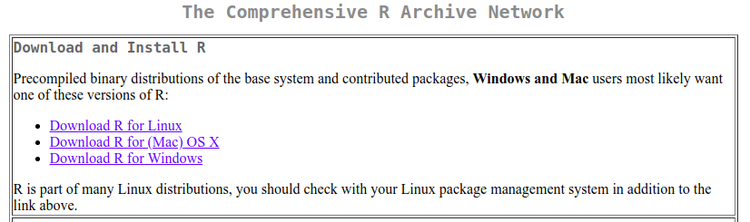
\includegraphics[width=1\linewidth]{downloadR} \end{center}

Siga as instruções para a instalação, diferentes para cada sistema
operacional.

\hypertarget{instalauxe7uxe3o-do-rstudio}{%
\subsubsection{Instalação do
RStudio}\label{instalauxe7uxe3o-do-rstudio}}

Uma vez instalada a linguagem R, você pode instalar o RStudio. O
procedimento, novamente, depende do sistema operacional. O RStudio
funciona nos três: Linux, Macintosh e Windows.

No site oficial do RStudio,
\url{https://www.rstudio.com/products/rstudio/download/}, encontrará o
que precisa. Pegue a versão gratuita do \textbf{RStudio Desktop}.

\hypertarget{uxe1reas-da-tela-no-rstudio}{%
\subsection{Áreas da tela no
RStudio}\label{uxe1reas-da-tela-no-rstudio}}

Ao entrar no RStudio, encontrará a uma tela como esta:

\begin{center}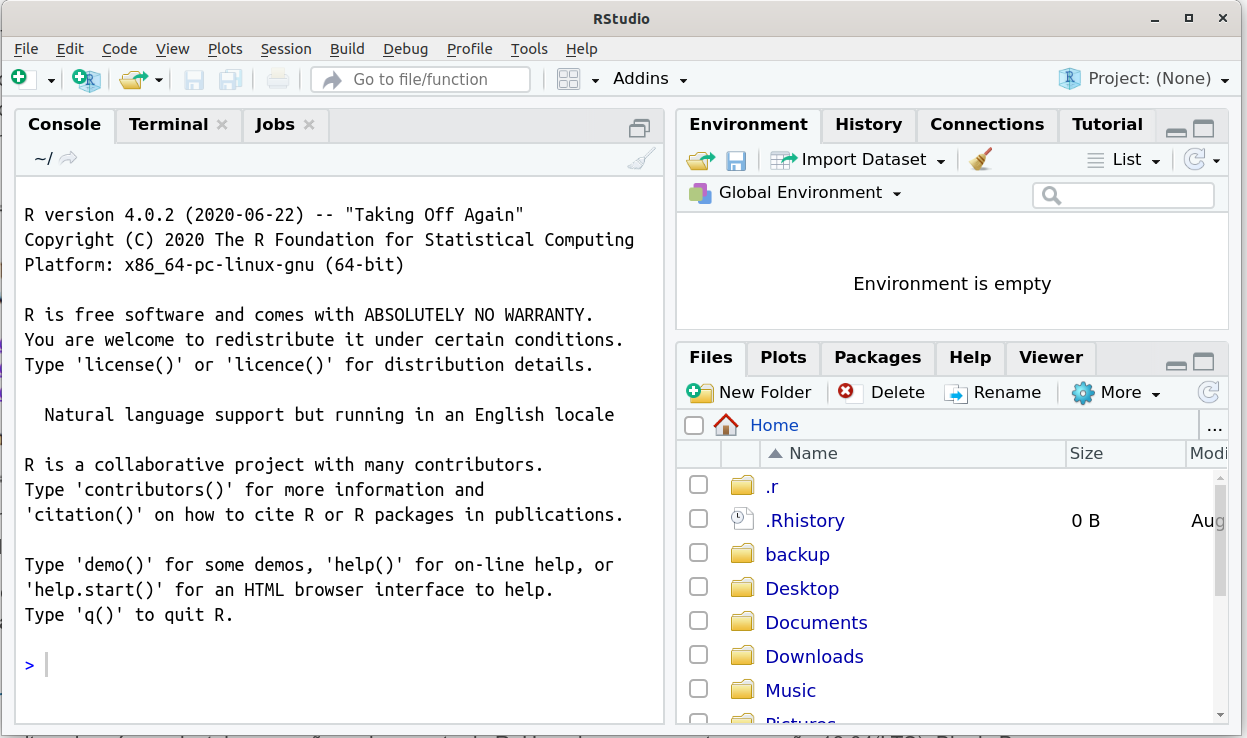
\includegraphics[width=0.9\linewidth]{RStudio_firstscreen} \end{center}

Reconheça os seguintes elementos:

\begin{itemize}
\tightlist
\item
  uma área com as abas \emph{Console} e \emph{Terminal}. Usaremos a
  \emph{Console} sempre (o terminal serve para usos mais avançados e
  desnecessários para nosso contexto). A console permite que usemos
  comandos diretos em R (veremos adiante).
\item
  uma área com as abas \emph{Environment} (ambiente), \emph{History}
  (histórico) e \emph{Connections} (conexões). Usaremos principalmente o
  ambiente, onde as variáveis ativas aparecem (as veremos em ação
  adiante).
\item
  uma área com as abas \emph{Files} (arquivos), \emph{Plots} (gráficos),
  \emph{Packages} (pacotes), \emph{Help} (ajuda) e \emph{Viewer}
  (visualizador). Os dois primeiros e a área de ajuda são os mais
  importantes para começar.
\end{itemize}

\hypertarget{comeuxe7ando-a-usar-a-console}{%
\subsection{\texorpdfstring{Começando a usar a
\emph{Console}}{Começando a usar a Console}}\label{comeuxe7ando-a-usar-a-console}}

É através da \emph{Console} que usamos comandos para o R. Vamos
experimentar algumas coisas simples, para começar.

O símbolo \textgreater{} é o \emph{prompt} do R, indicando que está
pronto para receber uma instrução qualquer. Por exemplo, podemos fazer
uma conta digitando na \emph{Console} (digite após o símbolo
\textgreater{} e pressione {[}enter{]} ao final da linha):

\begin{Shaded}
\begin{Highlighting}[]
\DecValTok{4}\SpecialCharTok{+}\DecValTok{5}
\end{Highlighting}
\end{Shaded}

obtendo

\begin{verbatim}
[1] 9
\end{verbatim}

A soma de quatro e cinco resulta em 9.

Podemos guardar os valores em \textbf{variáveis} (pressione {[}enter{]}
ao final de cada linha):

\begin{Shaded}
\begin{Highlighting}[]
\NormalTok{a }\OtherTok{\textless{}{-}} \DecValTok{4}
\NormalTok{b }\OtherTok{\textless{}{-}} \DecValTok{5}
\NormalTok{a }\SpecialCharTok{+}\NormalTok{ b}
\end{Highlighting}
\end{Shaded}

\begin{verbatim}
[1] 9
\end{verbatim}

Dando nomes, a e b são variáveis que receberam (com o operador de
atribuição, \textless-) os valores 4 e 5, respectivamente. Sua soma, a +
b (+ é o operador da adição), é 9. Podemos guardar este resultado em uma
outra variável:

\begin{Shaded}
\begin{Highlighting}[]
\NormalTok{soma }\OtherTok{\textless{}{-}}\NormalTok{ a }\SpecialCharTok{+}\NormalTok{ b}
\end{Highlighting}
\end{Shaded}

e podemos ecoar o conteúdo da variável soma, simplesmente escrevendo seu
nome:

\begin{Shaded}
\begin{Highlighting}[]
\NormalTok{soma}
\end{Highlighting}
\end{Shaded}

\begin{verbatim}
[1] 9
\end{verbatim}

\begin{center}\rule{0.5\linewidth}{0.5pt}\end{center}

\begin{flushleft}
\includegraphics[width=0.08\linewidth]{coruja} \end{flushleft}

Observe que nomes de variáveis podem ter várias letras e números (desde
que comece com letra). Não use letras acentuadas e tenha cuidado com a
grafia porque o R distingue maiúsculas de minúsculas: soma, Soma e SOMA
são variáveis diferentes, cada uma criada com conteúdo independente.

Nomes como soma\_1, Soma\_b, x ou A são, também, nomes válidos para
variáveis. Crie variáveis com nomes que facilitem, para você, lembrar o
tipo de conteúdo depositado nelas.

\begin{center}\rule{0.5\linewidth}{0.5pt}\end{center}

O resultado armazenado na variável soma pode ser usado:

\begin{Shaded}
\begin{Highlighting}[]
\NormalTok{raiz }\OtherTok{\textless{}{-}} \FunctionTok{sqrt}\NormalTok{(soma)}
\NormalTok{raiz}
\end{Highlighting}
\end{Shaded}

\begin{verbatim}
[1] 3
\end{verbatim}

Neste exemplo, pela primeira vez, usamos uma função, sqrt(), que extrai
a raiz quadrada (\emph{square root}, em inglês) de soma e a armazena em
outra variável, raiz. O R distingue variáveis de funções porque as
funções recebem parâmetros (neste caso, um valor numérico contido em
soma) entre parênteses. A função sqrt() faz parte do conjunto de funções
básicas do R.

\begin{center}\rule{0.5\linewidth}{0.5pt}\end{center}

\begin{flushleft}
\includegraphics[width=0.08\linewidth]{coruja} \end{flushleft}

Nada impede a criação de uma variável chamada sqrt, mas não é
recomendável. O R não confundirá, mas você sim. Uma possível sugestão,
se você não pretende distribuir seu código internacionalmente, é dar
nomes em português para as variáveis (e.g., raiz\_quadrada); outra opção
é usar algum tipo de prefixo (e.g., v\_sqrt ou v.sqrt).

\begin{center}\rule{0.5\linewidth}{0.5pt}\end{center}

Usar a console desta forma só é útil para tarefas pequenas ou testes
para acertar a sintaxe. Adiante veremos como colocar vários comandos em
um \emph{Rscript} e, mais sofisticadamente, em uma função, usando
decisões ou \emph{loops}, para facilitar seu trabalho. Por exemplo,
apenas como um ``aperitivo'', experimente um \emph{loop}:

\begin{Shaded}
\begin{Highlighting}[]
\ControlFlowTok{for}\NormalTok{ (n }\ControlFlowTok{in} \DecValTok{0}\SpecialCharTok{:}\DecValTok{10}\NormalTok{) }
\NormalTok{\{}
  \FunctionTok{cat}\NormalTok{(n,}\StringTok{"x 3 ="}\NormalTok{,n}\SpecialCharTok{*}\DecValTok{3}\NormalTok{,}\StringTok{"}\SpecialCharTok{\textbackslash{}n}\StringTok{"}\NormalTok{)}
\NormalTok{\}}
\end{Highlighting}
\end{Shaded}

\begin{verbatim}
0 x 3 = 0 
1 x 3 = 3 
2 x 3 = 6 
3 x 3 = 9 
4 x 3 = 12 
5 x 3 = 15 
6 x 3 = 18 
7 x 3 = 21 
8 x 3 = 24 
9 x 3 = 27 
10 x 3 = 30 
\end{verbatim}

É um \emph{loop} (usando a palavra reservada for) no qual a variável n
vai de 0 a 10, usa o operador de multiplicação, *, e exibe a tabuada do
3 com um único comando.

Em muitas situações podemos evitar \emph{loops} deste tipo, lançando mão
de intervalos com o operador :, ou fazendo operações sobre vetores ou
\emph{data frames} inteiros.

Por exemplo, a tabuada acima pode ser obtida com:

\begin{Shaded}
\begin{Highlighting}[]
\FunctionTok{paste}\NormalTok{(}\DecValTok{0}\SpecialCharTok{:}\DecValTok{10}\NormalTok{,}\StringTok{"x 3 ="}\NormalTok{,(}\DecValTok{0}\SpecialCharTok{:}\DecValTok{10}\NormalTok{)}\SpecialCharTok{*}\DecValTok{3}\NormalTok{)}
\end{Highlighting}
\end{Shaded}

\begin{verbatim}
 [1] "0 x 3 = 0"   "1 x 3 = 3"   "2 x 3 = 6"   "3 x 3 = 9"   "4 x 3 = 12" 
 [6] "5 x 3 = 15"  "6 x 3 = 18"  "7 x 3 = 21"  "8 x 3 = 24"  "9 x 3 = 27" 
[11] "10 x 3 = 30"
\end{verbatim}

Entenda o código. A instrução 0:10 gera

\begin{Shaded}
\begin{Highlighting}[]
\DecValTok{0}\SpecialCharTok{:}\DecValTok{10}
\end{Highlighting}
\end{Shaded}

\begin{verbatim}
 [1]  0  1  2  3  4  5  6  7  8  9 10
\end{verbatim}

e a função paste() concatena o que está dentro dela, sendo chamada 11
vezes por causa 0:10, variando os números e mantendo a parte fixa entre
aspas, ``x 3 =''.

Variáveis podem conter listas de valores. A mais simples são
\textbf{vetores}, criadas com a função de contatenação, c():

\begin{Shaded}
\begin{Highlighting}[]
\NormalTok{vetor }\OtherTok{\textless{}{-}} \FunctionTok{c}\NormalTok{(}\DecValTok{0}\NormalTok{,}\DecValTok{1}\NormalTok{,}\DecValTok{2}\NormalTok{,}\DecValTok{3}\NormalTok{,}\DecValTok{4}\NormalTok{,}\DecValTok{5}\NormalTok{,}\DecValTok{6}\NormalTok{,}\DecValTok{7}\NormalTok{,}\DecValTok{8}\NormalTok{,}\DecValTok{9}\NormalTok{,}\DecValTok{10}\NormalTok{)}
\NormalTok{vetor}
\end{Highlighting}
\end{Shaded}

\begin{verbatim}
 [1]  0  1  2  3  4  5  6  7  8  9 10
\end{verbatim}

ou, o que é o mesmo,

\begin{Shaded}
\begin{Highlighting}[]
\NormalTok{vetor }\OtherTok{\textless{}{-}} \DecValTok{0}\SpecialCharTok{:}\DecValTok{10}
\NormalTok{vetor}
\end{Highlighting}
\end{Shaded}

\begin{verbatim}
 [1]  0  1  2  3  4  5  6  7  8  9 10
\end{verbatim}

Vetores permitem operações ``em lote'', por exemplo, mostrando os
resultados da tabuada do 3 sem precisar do \emph{loop}:

\begin{Shaded}
\begin{Highlighting}[]
\NormalTok{vetor }\SpecialCharTok{*} \DecValTok{3}
\end{Highlighting}
\end{Shaded}

\begin{verbatim}
 [1]  0  3  6  9 12 15 18 21 24 27 30
\end{verbatim}

Em R, como vetor tem 11 valores, a multiplicação por 3 será repetida
para cada um deles, e 11 resultados (de 3x0 a 3x10) serão computados.
Porém, perdemos o formato da tabuada. Funções podem ser aninhadas:

\begin{Shaded}
\begin{Highlighting}[]
\NormalTok{vetor }\OtherTok{\textless{}{-}} \DecValTok{0}\SpecialCharTok{:}\DecValTok{10}
\NormalTok{tabuada }\OtherTok{\textless{}{-}} \FunctionTok{paste}\NormalTok{(vetor,}\StringTok{"x"}\NormalTok{,}\DecValTok{3}\NormalTok{,}\StringTok{"="}\NormalTok{,vetor}\SpecialCharTok{*}\DecValTok{3}\NormalTok{)}
\NormalTok{m }\OtherTok{\textless{}{-}} \FunctionTok{matrix}\NormalTok{(}\AttributeTok{data=}\NormalTok{tabuada, }\AttributeTok{ncol=}\DecValTok{1}\NormalTok{, }\AttributeTok{nrow=}\DecValTok{11}\NormalTok{)}
\FunctionTok{prmatrix}\NormalTok{(m, }\AttributeTok{collab=}\StringTok{""}\NormalTok{, }\AttributeTok{rowlab=}\FunctionTok{rep}\NormalTok{(}\StringTok{""}\NormalTok{,}\DecValTok{11}\NormalTok{), }\AttributeTok{quote=}\ConstantTok{FALSE}\NormalTok{)}
\end{Highlighting}
\end{Shaded}

\begin{verbatim}
            
 0 x 3 = 0  
 1 x 3 = 3  
 2 x 3 = 6  
 3 x 3 = 9  
 4 x 3 = 12 
 5 x 3 = 15 
 6 x 3 = 18 
 7 x 3 = 21 
 8 x 3 = 24 
 9 x 3 = 27 
 10 x 3 = 30
\end{verbatim}

A função prmatrix() imprime uma matriz. Matrizes podem ser criadas
quando queremos uma coleção de valores com duas dimensões (o vetor é
unidimensional), cujos elementos individuais são todos do mesmo tipo
(neste exemplo, \emph{strings} alfanuméricas) endereçados por
{[}linha,coluna{]}. Neste exemplo, linha vai de 1 a 11, mas só existe
uma coluna. Para ver, por exemplo, o conteúdo da terceira linha, podemos
usar

\begin{Shaded}
\begin{Highlighting}[]
\FunctionTok{cat}\NormalTok{(}\StringTok{"A terceira linha contém"}\NormalTok{,m[}\DecValTok{3}\NormalTok{,}\DecValTok{1}\NormalTok{],}\StringTok{"}\SpecialCharTok{\textbackslash{}n}\StringTok{"}\NormalTok{)}
\end{Highlighting}
\end{Shaded}

\begin{verbatim}
A terceira linha contém 2 x 3 = 6 
\end{verbatim}

\begin{center}\rule{0.5\linewidth}{0.5pt}\end{center}

\begin{flushleft}
\includegraphics[width=0.08\linewidth]{coruja} \end{flushleft}

As funções cat(), print() e prmatrix() que usamos até aqui têm
comportamentos similares em várias situações, mas diferentes em outras.
A mais simples é cat(). Repare que existe um ``\textbackslash n'', que
tem pouco efeito aqui mas é importante em \emph{Rscripts}. O efeito de
``\textbackslash n'' é de \emph{carriage return}, similar ao que ocorre
quando pressiona {[}enter{]} em um processador de textos para continuar
escrevendo na próxima linha (aparecerão exemplos adiante).

Note, também, que um espaço foi adicionado após a palavra ``contém''.

\begin{Shaded}
\begin{Highlighting}[]
\FunctionTok{cat}\NormalTok{(}\StringTok{"A terceira linha contém"}\NormalTok{,m[}\DecValTok{3}\NormalTok{,}\DecValTok{1}\NormalTok{],}\StringTok{"}\SpecialCharTok{\textbackslash{}n}\StringTok{"}\NormalTok{)}
\end{Highlighting}
\end{Shaded}

\begin{verbatim}
A terceira linha contém 2 x 3 = 6 
\end{verbatim}

Isto nem sempre é desejado, quando colocamos os espaços do nosso jeito e
não queremos a interferência da função, que inclui um espaço em branco
como separador por \emph{default}. Podemos mudar o separador com o
parâmetro sep() e escrever:

\begin{Shaded}
\begin{Highlighting}[]
\FunctionTok{cat}\NormalTok{(}\StringTok{"A terceira linha contém "}\NormalTok{,m[}\DecValTok{3}\NormalTok{,}\DecValTok{1}\NormalTok{],}\StringTok{"}\SpecialCharTok{\textbackslash{}n}\StringTok{"}\NormalTok{,}\AttributeTok{sep=}\StringTok{""}\NormalTok{)}
\end{Highlighting}
\end{Shaded}

\begin{verbatim}
A terceira linha contém 2 x 3 = 6
\end{verbatim}

(o separador é vazio e o espaço após ``contém'' foi explicitamente
colocado dentro das aspas).

O equivalente com a função print() precisa da ajuda de paste() mas não
precisa de ``\textbackslash n'' (pois print() já termina mudando de
linha):

\begin{Shaded}
\begin{Highlighting}[]
\FunctionTok{print}\NormalTok{(}\FunctionTok{paste}\NormalTok{(}\StringTok{"A terceira linha contém "}\NormalTok{,m[}\DecValTok{3}\NormalTok{,}\DecValTok{1}\NormalTok{],}\AttributeTok{sep=}\StringTok{""}\NormalTok{))}
\end{Highlighting}
\end{Shaded}

\begin{verbatim}
[1] "A terceira linha contém 2 x 3 = 6"
\end{verbatim}

A função print() ``suja'' o início da linha com {[}1{]} e não é a mais
indicada para uma saída destinada a quem não é usuário do R e não sabe o
que isto significa. No entanto, print() consegue exibir estruturas mais
complexas, como por exemplo a matriz m que definimos acima. Compare:

\begin{Shaded}
\begin{Highlighting}[]
\FunctionTok{cat}\NormalTok{(m,}\StringTok{"}\SpecialCharTok{\textbackslash{}n}\StringTok{"}\NormalTok{)}
\end{Highlighting}
\end{Shaded}

\begin{verbatim}
0 x 3 = 0 1 x 3 = 3 2 x 3 = 6 3 x 3 = 9 4 x 3 = 12 5 x 3 = 15 6 x 3 = 18 7 x 3 = 21 8 x 3 = 24 9 x 3 = 27 10 x 3 = 30 
\end{verbatim}

com

\begin{Shaded}
\begin{Highlighting}[]
\FunctionTok{print}\NormalTok{(m)}
\end{Highlighting}
\end{Shaded}

\begin{verbatim}
      [,1]         
 [1,] "0 x 3 = 0"  
 [2,] "1 x 3 = 3"  
 [3,] "2 x 3 = 6"  
 [4,] "3 x 3 = 9"  
 [5,] "4 x 3 = 12" 
 [6,] "5 x 3 = 15" 
 [7,] "6 x 3 = 18" 
 [8,] "7 x 3 = 21" 
 [9,] "8 x 3 = 24" 
[10,] "9 x 3 = 27" 
[11,] "10 x 3 = 30"
\end{verbatim}

Por fim, prmatrix() é uma especialização de print(), com parâmetros que
podem ocultar os endereçamentos das linhas e colunas, como fizemos com

\begin{Shaded}
\begin{Highlighting}[]
\FunctionTok{prmatrix}\NormalTok{(m, }\AttributeTok{collab=}\StringTok{""}\NormalTok{, }\AttributeTok{rowlab=}\FunctionTok{rep}\NormalTok{(}\StringTok{""}\NormalTok{,}\DecValTok{11}\NormalTok{), }\AttributeTok{quote=}\ConstantTok{FALSE}\NormalTok{)}
\end{Highlighting}
\end{Shaded}

\begin{verbatim}
            
 0 x 3 = 0  
 1 x 3 = 3  
 2 x 3 = 6  
 3 x 3 = 9  
 4 x 3 = 12 
 5 x 3 = 15 
 6 x 3 = 18 
 7 x 3 = 21 
 8 x 3 = 24 
 9 x 3 = 27 
 10 x 3 = 30
\end{verbatim}

substituindo os rótulos (\emph{labels}, em inglês) das colunas (collab)
e linhas (rowlab) por um vazio, além de não exibir aspas (quote=FALSE).
Experimente alterar estes parâmetros para ver o que acontece.

\begin{center}\rule{0.5\linewidth}{0.5pt}\end{center}

\hypertarget{criando-um-projeto}{%
\subsubsection{Criando um projeto}\label{criando-um-projeto}}

\textbf{Antes} de fazer qualquer coisa \textbf{recomendamos SEMPRE
iniciar um Projeto}. Repare no canto superior-direito da tela que existe
um menu mostrando que não há um projeto aberto (veja, por exemplo, a
tela do RStudio acima).

\begin{center}\rule{0.5\linewidth}{0.5pt}\end{center}

\begin{flushleft}
\includegraphics[width=0.08\linewidth]{coruja} \end{flushleft}

O principal motivo para criar um projeto é a organização. O projeto
reserva uma pasta, dentro da qual ficarão os \emph{Rscripts} que
desenvolverá, os arquivos com dados ou resultados, ou o que mais você
fizer pertinentemente ao projeto.

\begin{center}\rule{0.5\linewidth}{0.5pt}\end{center}

Para criar um projeto novo no RStudio, no canto superior-direito clique
em \emph{New project} e aponte-o para uma pasta de sua preferência (ou
crie uma pasta nova). Terá, também, que dar um nome ao projeto. Neste
exemplo vou chamá-lo de \emph{\textbf{Anticoncepcional}}.

\begin{center}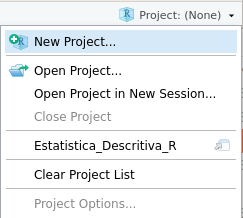
\includegraphics[width=0.9\linewidth]{RStudio_criaprojeto} \end{center}

Você pode apontar uma pasta existente ou criar uma nova através do
próprio RStudio. No caso de pasta nova, chegará em uma tela assim:

\begin{center}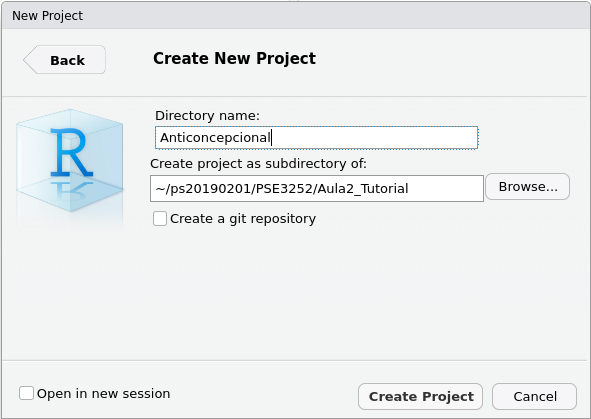
\includegraphics[width=0.9\linewidth]{RStudio_projetonovo} \end{center}

O nome do diretório (sinônimo de pasta) será a pasta nova e, também, o
nome do projeto. A segunda parte é sob qual pasta seu projeto ficará
subordinado.

\begin{center}\rule{0.5\linewidth}{0.5pt}\end{center}

\begin{flushleft}
\includegraphics[width=0.08\linewidth]{coruja} \end{flushleft}

Em meu caso uso o RStudio em \emph{Linux}, e este sistema operacional
endereça as pastas com sua própria sintaxe, separando os níveis por
\emph{slash} (`/'). No Windows aparecerão caminhos como
``C:\textbackslash Meus Documentos\textbackslash\ldots{}'', separando os
níveis por \emph{backslash} (`\textbackslash{}')).

\begin{center}\rule{0.5\linewidth}{0.5pt}\end{center}

O RStudio, na pasta que você apontar, criará o arquivo
\emph{Anticoncepcional.Rproj} e mostrará, na janela inferior-direita, o
caminho até a pasta apontada e os arquivos que ela contém na aba
\emph{Files}.

\begin{center}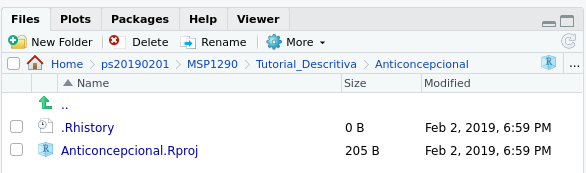
\includegraphics[width=0.9\linewidth]{RStudio_files} \end{center}

Neste exemplo, como criei uma pasta nova, só aparece nela (por enquanto)
o que o RStudio criou para mim.

\hypertarget{criando-um-rscript}{%
\subsubsection{\texorpdfstring{Criando um
\emph{Rscript}}{Criando um Rscript}}\label{criando-um-rscript}}

Vamos aproveitar o que testamos na \emph{Console} para ilustrar como
guardá-lo junto ao projeto que acabamos de criar.

Use o menu e selecione

\emph{File -\textgreater{} New file -\textgreater{} Rscript}

(que, no meu sistema, pode ser substituído por um ``atalho'' pelo
teclado, pressionando as teclas Ctrl+Shift+N, simultaneamente).

\begin{center}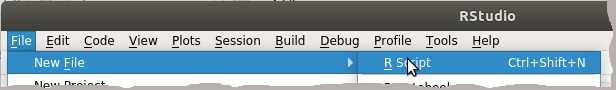
\includegraphics[width=0.9\linewidth]{RStudio_RScriptnovo} \end{center}

Uma nova aba, chamada \emph{Untitled1} deve abrir-se:

\begin{center}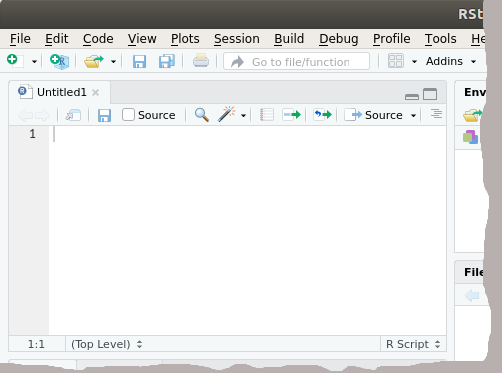
\includegraphics[width=0.9\linewidth]{RStudio_newfile} \end{center}

Coloque, dentro desta nova área, a tabuada do 3 que ensaiamos acima,
digitando:

\begin{Shaded}
\begin{Highlighting}[]
\CommentTok{\# Este é meu primeiro Rscript}
\FunctionTok{cat}\NormalTok{(}\StringTok{"Apresentando a tabuada do 3}\SpecialCharTok{\textbackslash{}n}\StringTok{"}\NormalTok{)}
\ControlFlowTok{for}\NormalTok{ (n }\ControlFlowTok{in} \DecValTok{0}\SpecialCharTok{:}\DecValTok{10}\NormalTok{) }
\NormalTok{\{}
  \FunctionTok{cat}\NormalTok{(n,}\StringTok{"x"}\NormalTok{,}\DecValTok{3}\NormalTok{,}\StringTok{"="}\NormalTok{,n}\SpecialCharTok{*}\DecValTok{3}\NormalTok{,}\StringTok{"}\SpecialCharTok{\textbackslash{}n}\StringTok{"}\NormalTok{)}
\NormalTok{\}}
\end{Highlighting}
\end{Shaded}

\begin{center}\rule{0.5\linewidth}{0.5pt}\end{center}

\begin{flushleft}
\includegraphics[width=0.08\linewidth]{coruja} \end{flushleft}

Entenda a sintaxe do R:

\begin{itemize}
\tightlist
\item
  O símbolo de \emph{hashtag} (\#) indica uma linha de comentário (algo
  para você lembrar o que faz determinado trecho de um \emph{Rscript},
  que não será executada).
\item
  cat() é uma função R que ecoa na Console o texto que for passado como
  parâmetro; neste exemplo, o primeiro cat() apenas escreve
  ``Apresentando a tabuada do 3'' e avança uma linha (por causa do
  caracter especial \textbackslash n).
\item
  o for() já foi apresentado, e faz a variável n assumir sequencialmente
  os valores 0, 1, 2, \ldots, 10.
\item
  tudo que está entre as chaves, \{\ldots\}, é executado repetidamente a
  cada ciclo do for().
\item
  este segundo cat tem parte do texto fixo com parte variável, ecoando o
  resultado de cada multiplicação, uma em cada linha.
\end{itemize}

\begin{center}\rule{0.5\linewidth}{0.5pt}\end{center}

Salve seu \emph{Rscript} na mesma pasta em que está o projeto, usando

\emph{File -\textgreater{} Save}

com o nome \emph{tabuada3.R}. Agora a aba tem o nome do arquivo que
acabou de ser criado.

\begin{center}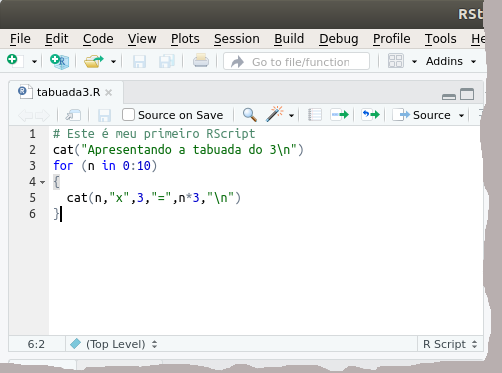
\includegraphics[width=0.9\linewidth]{RStudio_RScriptsalvo} \end{center}

Execute seu \emph{Rscript} clicando o botão {[}Source{]} e observe o
resultado na \emph{Console}

\begin{verbatim}
Apresentando a tabuada do 3
\end{verbatim}

\begin{verbatim}
0 x 3 = 0 
1 x 3 = 3 
2 x 3 = 6 
3 x 3 = 9 
4 x 3 = 12 
5 x 3 = 15 
6 x 3 = 18 
7 x 3 = 21 
8 x 3 = 24 
9 x 3 = 27 
10 x 3 = 30 
\end{verbatim}

Um uso um pouco mais avançado é a criação de funções. Você não precisa
se contentar com as milhares de funções já disponíveis em R. A linguagem
é expansível, e você pode criar mais funções. É assim que R, com a
cooperação de muitas pessoas, cresce continuamente.

Por exemplo, podemos criar uma função chamada tabuada() assim:

\begin{Shaded}
\begin{Highlighting}[]
\NormalTok{tabuada }\OtherTok{\textless{}{-}} \ControlFlowTok{function}\NormalTok{ (}\AttributeTok{multiplicando=}\DecValTok{1}\NormalTok{)}
\NormalTok{\{}
  \FunctionTok{cat}\NormalTok{(}\StringTok{"Apresentando a tabuada do "}\NormalTok{,multiplicando,}\StringTok{":}\SpecialCharTok{\textbackslash{}n}\StringTok{"}\NormalTok{, }\AttributeTok{sep=}\StringTok{""}\NormalTok{)}
  \ControlFlowTok{for}\NormalTok{ (n }\ControlFlowTok{in} \DecValTok{0}\SpecialCharTok{:}\DecValTok{10}\NormalTok{) }
\NormalTok{  \{}
    \FunctionTok{cat}\NormalTok{(n,}\StringTok{"x"}\NormalTok{,multiplicando,}\StringTok{"="}\NormalTok{,n}\SpecialCharTok{*}\NormalTok{multiplicando,}\StringTok{"}\SpecialCharTok{\textbackslash{}n}\StringTok{"}\NormalTok{)}
\NormalTok{  \}}
\NormalTok{\}}
\end{Highlighting}
\end{Shaded}

Salve este \emph{Rscript} com o nome de tabuada.R. Rode este
\emph{Rscript} com {[}Source{]} uma única vez para que a função
tabuada() fique disponível na memória. Esta função recebe um parâmetro,
o multiplicando. Caso nenhum parâmetro seja passado, a declaração da
função tem o valor 1 como \emph{default} (multiplicando=1). Passando
qualquer outro valor, aparecerá a tabuada solicitada. Por exemplo,
experimente com a \emph{Console} várias possibilidades:

\begin{Shaded}
\begin{Highlighting}[]
\FunctionTok{tabuada}\NormalTok{()}
\end{Highlighting}
\end{Shaded}

\begin{verbatim}
Apresentando a tabuada do 1:
0 x 1 = 0 
1 x 1 = 1 
2 x 1 = 2 
3 x 1 = 3 
4 x 1 = 4 
5 x 1 = 5 
6 x 1 = 6 
7 x 1 = 7 
8 x 1 = 8 
9 x 1 = 9 
10 x 1 = 10 
\end{verbatim}

\begin{Shaded}
\begin{Highlighting}[]
\FunctionTok{tabuada}\NormalTok{(}\AttributeTok{multiplicando=}\DecValTok{5}\NormalTok{)}
\end{Highlighting}
\end{Shaded}

\begin{verbatim}
Apresentando a tabuada do 5:
0 x 5 = 0 
1 x 5 = 5 
2 x 5 = 10 
3 x 5 = 15 
4 x 5 = 20 
5 x 5 = 25 
6 x 5 = 30 
7 x 5 = 35 
8 x 5 = 40 
9 x 5 = 45 
10 x 5 = 50 
\end{verbatim}

\begin{Shaded}
\begin{Highlighting}[]
\FunctionTok{tabuada}\NormalTok{(}\DecValTok{8}\NormalTok{)}
\end{Highlighting}
\end{Shaded}

\begin{verbatim}
Apresentando a tabuada do 8:
0 x 8 = 0 
1 x 8 = 8 
2 x 8 = 16 
3 x 8 = 24 
4 x 8 = 32 
5 x 8 = 40 
6 x 8 = 48 
7 x 8 = 56 
8 x 8 = 64 
9 x 8 = 72 
10 x 8 = 80 
\end{verbatim}

\begin{Shaded}
\begin{Highlighting}[]
\FunctionTok{tabuada}\NormalTok{(}\SpecialCharTok{{-}}\DecValTok{2}\NormalTok{)}
\end{Highlighting}
\end{Shaded}

\begin{verbatim}
Apresentando a tabuada do -2:
0 x -2 = 0 
1 x -2 = -2 
2 x -2 = -4 
3 x -2 = -6 
4 x -2 = -8 
5 x -2 = -10 
6 x -2 = -12 
7 x -2 = -14 
8 x -2 = -16 
9 x -2 = -18 
10 x -2 = -20 
\end{verbatim}

Esta função recebe somente um parâmetro e não retorna valores. Podemos
melhorá-la, guardando a tabuada em uma matriz e retornando-a para que
seus valores possam ser usados separadamente e/ou manipulados por outras
partes de um \emph{Rscript}. Por exemplo:

\begin{Shaded}
\begin{Highlighting}[]
\NormalTok{tabuada }\OtherTok{\textless{}{-}} \ControlFlowTok{function}\NormalTok{ (}\AttributeTok{multiplicando=}\DecValTok{1}\NormalTok{, }\AttributeTok{echo=}\ConstantTok{TRUE}\NormalTok{)}
\NormalTok{\{}
  \ControlFlowTok{if}\NormalTok{ (echo)}
\NormalTok{  \{}
    \FunctionTok{cat}\NormalTok{(}\StringTok{"Tabuada do "}\NormalTok{,multiplicando,}\StringTok{"}\SpecialCharTok{\textbackslash{}n}\StringTok{"}\NormalTok{,}\AttributeTok{sep=}\StringTok{""}\NormalTok{)}
\NormalTok{  \}  }
\NormalTok{  matriz }\OtherTok{\textless{}{-}} \FunctionTok{matrix}\NormalTok{(}\AttributeTok{data=}\ConstantTok{NA}\NormalTok{, }\AttributeTok{ncol=}\DecValTok{4}\NormalTok{, }\AttributeTok{nrow=}\DecValTok{11}\NormalTok{)}
  \FunctionTok{colnames}\NormalTok{(matriz) }\OtherTok{\textless{}{-}} \FunctionTok{c}\NormalTok{(}\StringTok{"multiplicando"}\NormalTok{, }\StringTok{"multiplicado"}\NormalTok{, }\StringTok{"produto"}\NormalTok{, }\StringTok{"texto"}\NormalTok{)}
  \ControlFlowTok{for}\NormalTok{ (m }\ControlFlowTok{in} \FunctionTok{seq}\NormalTok{(}\AttributeTok{from=}\DecValTok{0}\NormalTok{,}\AttributeTok{to=}\DecValTok{10}\NormalTok{,}\AttributeTok{by=}\DecValTok{1}\NormalTok{))}
\NormalTok{  \{}
\NormalTok{    produto }\OtherTok{\textless{}{-}}\NormalTok{ m}\SpecialCharTok{*}\NormalTok{multiplicando}
\NormalTok{    matriz[m}\SpecialCharTok{+}\DecValTok{1}\NormalTok{,}\DecValTok{1}\NormalTok{] }\OtherTok{\textless{}{-}}\NormalTok{ m}
\NormalTok{    matriz[m}\SpecialCharTok{+}\DecValTok{1}\NormalTok{,}\DecValTok{2}\NormalTok{] }\OtherTok{\textless{}{-}}\NormalTok{ multiplicando}
\NormalTok{    matriz[m}\SpecialCharTok{+}\DecValTok{1}\NormalTok{,}\DecValTok{3}\NormalTok{] }\OtherTok{\textless{}{-}}\NormalTok{ produto}
\NormalTok{    matriz[m}\SpecialCharTok{+}\DecValTok{1}\NormalTok{,}\DecValTok{4}\NormalTok{] }\OtherTok{\textless{}{-}} \FunctionTok{paste}\NormalTok{(m,}\StringTok{"x"}\NormalTok{,multiplicando,}\StringTok{"="}\NormalTok{,produto,}\AttributeTok{sep=}\StringTok{""}\NormalTok{)}
    \ControlFlowTok{if}\NormalTok{ (echo)}
\NormalTok{    \{}
      \FunctionTok{cat}\NormalTok{(matriz[m}\SpecialCharTok{+}\DecValTok{1}\NormalTok{,}\DecValTok{4}\NormalTok{],}\StringTok{"}\SpecialCharTok{\textbackslash{}n}\StringTok{"}\NormalTok{)}
\NormalTok{    \}}
\NormalTok{  \}}
  \FunctionTok{return}\NormalTok{(matriz)}
\NormalTok{\}}
\end{Highlighting}
\end{Shaded}

Esta nova versão recebe dois parâmetros. O segundo, echo=TRUE, por
\emph{default} ecoa a tabuada enquanto a calcula. Caso passe echo=FALSE,
a função trabalhará ``em silêncio''. No entanto, retornará uma matriz
que tem quatro colunas, respectivamente contendo o número a ser
multiplicado (variando de 0 a 10), o multiplicando, o produto resultante
da multiplicação e uma \emph{string} alfanumérica que pode ser usada
para ecoar o resultado.

\begin{center}\rule{0.5\linewidth}{0.5pt}\end{center}

\begin{flushleft}
\includegraphics[width=0.08\linewidth]{coruja} \end{flushleft}

Esta função está implementada como eiras::times.tables. O pacote eiras
está disponível em \url{https://github.com/pspsilveira/eiras}.

(além das instruções no \textbf{github}, voltaremos a falar sobre
instalação de pacotes adiante)

\begin{center}\rule{0.5\linewidth}{0.5pt}\end{center}

Uma vez construída, esta função pode ser usada em outros
\emph{Rscripts}. Por exemplo, crie e salve o seguinte com o nome de
TesteTabuada.R:

\begin{Shaded}
\begin{Highlighting}[]
\FunctionTok{source}\NormalTok{ (}\StringTok{"tabuada.R"}\NormalTok{)}

\FunctionTok{cat}\NormalTok{(}\StringTok{"Chamando as tabuadas}\SpecialCharTok{\textbackslash{}n}\StringTok{"}\NormalTok{)}
\ControlFlowTok{for}\NormalTok{ (t }\ControlFlowTok{in} \DecValTok{0}\SpecialCharTok{:}\DecValTok{10}\NormalTok{)}
\NormalTok{\{}
\NormalTok{  m }\OtherTok{\textless{}{-}} \FunctionTok{tabuada}\NormalTok{(t, }\AttributeTok{echo=}\ConstantTok{FALSE}\NormalTok{)}
  \FunctionTok{cat}\NormalTok{(}\StringTok{"{-}Tabuada do "}\NormalTok{,t,}\StringTok{":}\SpecialCharTok{\textbackslash{}n}\StringTok{"}\NormalTok{,}\AttributeTok{sep=}\StringTok{""}\NormalTok{)}
  \FunctionTok{cat}\NormalTok{(}\StringTok{"}\SpecialCharTok{\textbackslash{}t}\StringTok{"}\NormalTok{,m[}\DecValTok{1}\SpecialCharTok{:}\FunctionTok{nrow}\NormalTok{(m),}\DecValTok{4}\NormalTok{],}\StringTok{"}\SpecialCharTok{\textbackslash{}n}\StringTok{"}\NormalTok{)}
\NormalTok{\}}
\end{Highlighting}
\end{Shaded}

A primeira linha coloca a função tabuada() na memória (tal como está
declarada dentro do arquivo tabuada.R). O nome da função e do arquivo
não precisam ser iguais e um arquivo pode conter a declaração de mais
que uma função. O restante do código chama tabuada() em silêncio,
trazendo seus resultados para a matriz m e, depois mostra apenas as
\emph{strings} armazenadas na quarta coluna com
as.character(m{[}r,4{]}). Execute-a com {[}Source{]} e veja seu
resultado na \emph{Console}:

\begin{verbatim}
Chamando as tabuadas
\end{verbatim}

\begin{verbatim}
-Tabuada do 0:
     0x0=0 1x0=0 2x0=0 3x0=0 4x0=0 5x0=0 6x0=0 7x0=0 8x0=0 9x0=0 10x0=0 
-Tabuada do 1:
     0x1=0 1x1=1 2x1=2 3x1=3 4x1=4 5x1=5 6x1=6 7x1=7 8x1=8 9x1=9 10x1=10 
-Tabuada do 2:
     0x2=0 1x2=2 2x2=4 3x2=6 4x2=8 5x2=10 6x2=12 7x2=14 8x2=16 9x2=18 10x2=20 
-Tabuada do 3:
     0x3=0 1x3=3 2x3=6 3x3=9 4x3=12 5x3=15 6x3=18 7x3=21 8x3=24 9x3=27 10x3=30 
-Tabuada do 4:
     0x4=0 1x4=4 2x4=8 3x4=12 4x4=16 5x4=20 6x4=24 7x4=28 8x4=32 9x4=36 10x4=40 
-Tabuada do 5:
     0x5=0 1x5=5 2x5=10 3x5=15 4x5=20 5x5=25 6x5=30 7x5=35 8x5=40 9x5=45 10x5=50 
-Tabuada do 6:
     0x6=0 1x6=6 2x6=12 3x6=18 4x6=24 5x6=30 6x6=36 7x6=42 8x6=48 9x6=54 10x6=60 
-Tabuada do 7:
     0x7=0 1x7=7 2x7=14 3x7=21 4x7=28 5x7=35 6x7=42 7x7=49 8x7=56 9x7=63 10x7=70 
-Tabuada do 8:
     0x8=0 1x8=8 2x8=16 3x8=24 4x8=32 5x8=40 6x8=48 7x8=56 8x8=64 9x8=72 10x8=80 
-Tabuada do 9:
     0x9=0 1x9=9 2x9=18 3x9=27 4x9=36 5x9=45 6x9=54 7x9=63 8x9=72 9x9=81 10x9=90 
-Tabuada do 10:
     0x10=0 1x10=10 2x10=20 3x10=30 4x10=40 5x10=50 6x10=60 7x10=70 8x10=80 9x10=90 10x10=100 
\end{verbatim}

Quando a execução terminar, a última tabuada estará na memória.
Experimente:

\begin{Shaded}
\begin{Highlighting}[]
\FunctionTok{print}\NormalTok{(m)}
\end{Highlighting}
\end{Shaded}

\begin{verbatim}
      multiplicando multiplicado produto texto      
 [1,] "0"           "10"         "0"     "0x10=0"   
 [2,] "1"           "10"         "10"    "1x10=10"  
 [3,] "2"           "10"         "20"    "2x10=20"  
 [4,] "3"           "10"         "30"    "3x10=30"  
 [5,] "4"           "10"         "40"    "4x10=40"  
 [6,] "5"           "10"         "50"    "5x10=50"  
 [7,] "6"           "10"         "60"    "6x10=60"  
 [8,] "7"           "10"         "70"    "7x10=70"  
 [9,] "8"           "10"         "80"    "8x10=80"  
[10,] "9"           "10"         "90"    "9x10=90"  
[11,] "10"          "10"         "100"   "10x10=100"
\end{verbatim}

Este objeto, m, pode ter seus elementos acessados. A quinta linha, por
exemplo,

\begin{Shaded}
\begin{Highlighting}[]
\FunctionTok{print}\NormalTok{(m[}\DecValTok{5}\NormalTok{,])}
\end{Highlighting}
\end{Shaded}

\begin{verbatim}
multiplicando  multiplicado       produto         texto 
          "4"          "10"          "40"     "4x10=40" 
\end{verbatim}

que pede a linha 5 e todas as colunas. Veremos melhor estes
endereçamentos de {[}linha,coluna{]} nos \emph{data frames}, adiante.

\begin{center}\rule{0.5\linewidth}{0.5pt}\end{center}

\begin{flushleft}
\includegraphics[width=0.08\linewidth]{coruja} \end{flushleft}

Como TesteTabuada.R não é uma função, seus valores estão acessíveis
depois que foi executado. As variáveis internas de uma função, no
entanto, não estão. Tente acessar, por exemplo, a variável matriz
construída dentro de tabuada.R e verá que não existe. As funções, uma
vez desenvolvidas, funcionam como ``caixas-pretas'', e seus conteúdos
ficam protegidos, de forma que não haverá conflito se variáveis externas
tiverem o mesmo nome daquelas usadas dentro de suas funções. O que
retornamos, neste exemplo, foi uma cópia da matriz para a variável m que
é, portanto, também uma matriz e podemos acessá-la.

\begin{center}\rule{0.5\linewidth}{0.5pt}\end{center}

\hypertarget{lendo-arquivos-de-dados}{%
\subsection{Lendo arquivos de dados}\label{lendo-arquivos-de-dados}}

Existem formas de ler vários tipos de arquivo com R. As duas formas mais
comuns são um arquivo texto que utilize algum tipo de delimitador
(vírgula, ponto e vírgula ou caracteres de tabulação são os mais
comuns), ou planilhas (o formato Excel, ``xls'' ou ``xlsx'' são os mais
difundidos).

Arquivos no formato texto são simples e completamente portáveis entre
diferentes sistemas operacionais. Há problemas, porém, com a comunicação
com pesquisadores menos habituados a eles: atrapalham-se com os
delimitadores, criam arquivos usando vírgulas como separador decimal
(misturando-os com vírgulas usadas como delimitadores e, assim,
bagunçando os dados de colunas diferentes), digitam números ora com
pontos decimais, ora com vírgulas (bagunçando os dados numéricos ao
transformar 1300 em 1.3 ou levar o sistema operacional a interpretar 1,3
como se fosse um texto) ou esquecem de especificar os delimitadores.

\hypertarget{arquivos-em-formato-texto}{%
\subsubsection{Arquivos em formato
texto}\label{arquivos-em-formato-texto}}

Para este exemplo lidaremos com um arquivo
\emph{\url{MetodoAnticoncepcional.txt}}, que deve ser baixado e colocado
na pasta do projeto. Ele aparecerá na lista de arquivos, junto aos
arquivos Anticoncepcional.Rproj e tabuada3.R mencionados acima. Este é
um exemplo hipotético, usando o seguinte enredo:

\begin{quote}
Um agente comunitário do programa de saúde da família deseja escrever um
pequeno texto alertando os jovens de sua comunidade sobre o problema da
gravidez indesejada. Com este propósito, ele decide investigar quais os
métodos que os jovens estão usando.
\end{quote}

\begin{quote}
Após pesquisa realizada com 60 jovens (14 -- 19 anos), escolhidos
aleatoriamente, obteve as respostas contidas em um arquivo texto.
\end{quote}

Este é um arquivo texto tem 61 linhas. A primeira linha tem os nomes das
colunas (que se tornarão os nomes das variáveis) e, em seguida, os dados
de cada indivíduo (um indivíduo em cada linha).

Você pode ter uma ideia do arquivo com a ajuda do RStudio: basta clicar
sobre ele na área de \emph{Files}, e o arquivo se abrirá em uma nova
janela à esquerda. Agora o RStudio mostra quatro áreas:

\begin{center}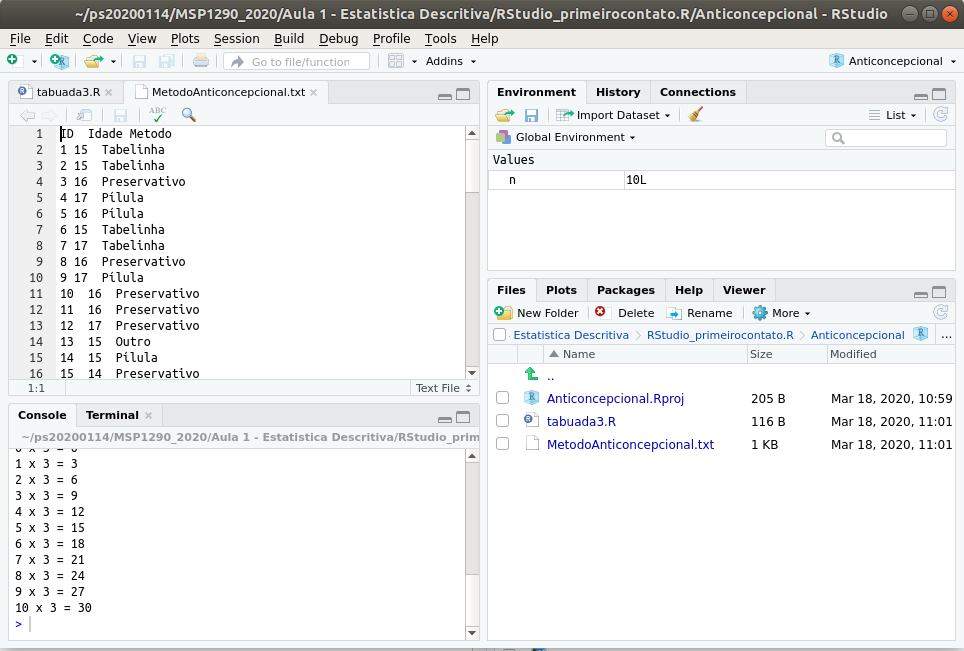
\includegraphics[width=0.9\linewidth]{RStudio_tsv} \end{center}

A \emph{Console} foi deslocada para baixo e o arquivo
\emph{MetodoAnticoncepcional.txt} está aberto em uma nova aba.

\begin{center}\rule{0.5\linewidth}{0.5pt}\end{center}

\begin{flushleft}
\includegraphics[width=0.08\linewidth]{coruja} \end{flushleft}

Este arquivo ainda não foi convertido a um formato com o qual R possa
lidar, tanto que as colunas parecem desalinhadas por causa dos conteúdos
com diferentes larguras. As colunas estão separadas por caracteres de
tabulação (\emph{tabs}, que normalmente têm a mesma aparência de um
espaço em branco, dando a impressão de que as colunas estão
desalinhadas, um dos motivos para a confusão que estes arquivos causam
para usuários ``\emph{não iniciados}'').

Repare, também, que não foram utilizadas letras acentuadas nos nomes das
variáveis (Metodo em vez de Método); caso o faça, poderá ter que lidar
com alguns problemas adicionais, especialmente quando seu sistema
operacional não for capaz de resolver sozinho, como acontece com o
\emph{Windows} (com o passar dos anos os problemas diminuiram, mas é
melhor não arriscar: sugere-se evitar acentos em nomes de variáveis e em
nomes de arquivos).

\begin{center}\rule{0.5\linewidth}{0.5pt}\end{center}

Variáveis, em R, podem ter estruturas mais elaboradas do que as que
contém apenas um valor ou um vetor com valores de mesma natureza.
Criaremos uma, chamada metodos, que conterá toda a informação que está
neste arquivo \emph{.txt} com o seguinte comando no console (janela à
esquerda):

\begin{Shaded}
\begin{Highlighting}[]
\NormalTok{metodos }\OtherTok{\textless{}{-}} \FunctionTok{read.table}\NormalTok{(}\StringTok{"MetodoAnticoncepcional.txt"}\NormalTok{, }
                         \AttributeTok{header=}\ConstantTok{TRUE}\NormalTok{,  }\AttributeTok{dec=}\StringTok{"."}\NormalTok{, }\AttributeTok{sep=}\StringTok{"}\SpecialCharTok{\textbackslash{}t}\StringTok{"}\NormalTok{)}
\end{Highlighting}
\end{Shaded}

Repare as especificações sobre o arquivo que foram passadas para a
função read.table():

\begin{itemize}
\tightlist
\item
  header=TRUE informa que a primeira linha deve ser usada como nome das
  variáveis;
\item
  dec=``.'' informa que ponto, se existir, é o separador decimal usado;
\item
  sep=``\textbackslash t'' informa o uso do tab como delimitador.
\end{itemize}

Outro formato comum de arquivo texto é o que recebe a extensão
\emph{.csv}, no qual as colunas são separadas por vírgula (\emph{comma})
ou ponto e vírgula (quando a vírgula já está usada para separar decimais
em língua portuguesa). O processo de importação é o mesmo, exceto que
precisará ajustar os parâmetros dec e sep adequadamente.

Na janela \emph{Environment} (superior-direita) aparece a variável
metodos, mostrando que a importação aconteceu. Clique no nome da
variável e na seta que aparece ao lado esquerdo do nome da variável para
ver algumas informações sobre seus detalhes, e sobre o nome da variável
para que o RStudio mostre-lhe seu conteúdo:

\begin{center}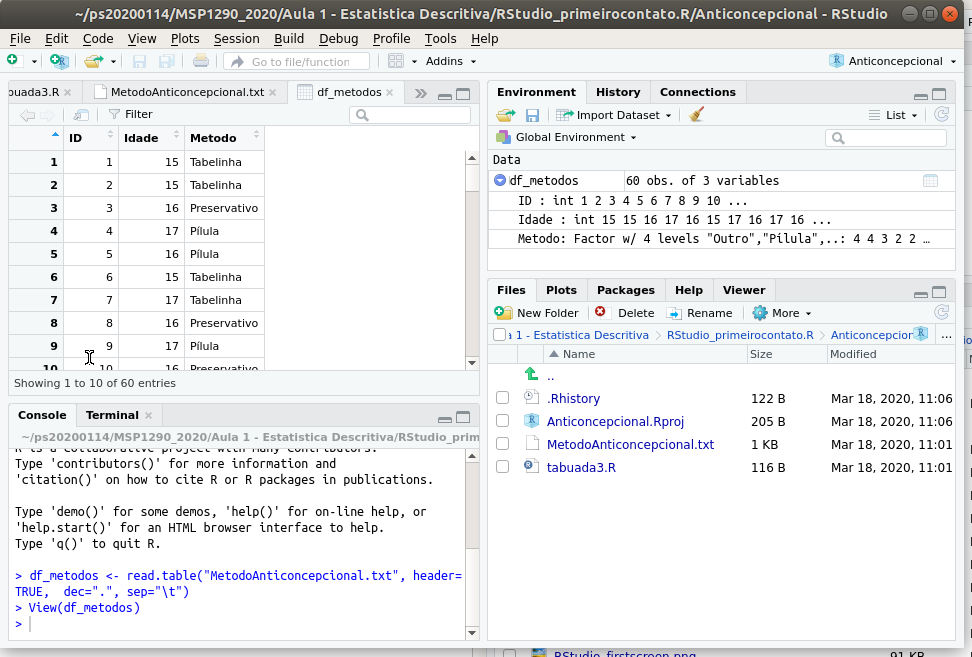
\includegraphics[width=0.9\linewidth]{RStudio_Tabela} \end{center}

Como pode observar, o RStudio lhe informa que metodos contém três
variáveis internas:

\begin{itemize}
\tightlist
\item
  ID, do tipo int (número inteiro, quantitativa)
\item
  Idade, do tipo int (número inteiro, quantitativa)
\item
  Metodo, fator com 4 níveis
\end{itemize}

A identificação do tipo de variável é automática, de acordo com o
conteúdo encontrado. Não havia números fracionários, então dec=``.'' não
era necessário (o símbolo usado como separador decimal - quem importa
arquivo texto precisa saber se os números foram escritos com a notação
inglesa, usando pontos, ou portuguesa, usando vírgulas). ID,
identificação do indivíduo, foi identificada como numérica, embora não o
seja, mas não atrapalha muito deixar assim por enquanto. Idade, ao
contrário, interessa como variável quantitativa, foi identificada como
tal, e podemos fazer cálculos com ela. A coluna Metodo foi reconhecida,
corretamente, como fator, i.e., pode ser usada para separar grupos. Como
é variável categórica (veremos, adiante, que são 4 categorias), podemos
fazer contagens.

Além de conhecer os tipos de variável de cada coluna, precisamos saber
qual é o tipo de metodos. Use (na \emph{Console}) o comando:

\begin{Shaded}
\begin{Highlighting}[]
\FunctionTok{is.table}\NormalTok{(metodos)}
\end{Highlighting}
\end{Shaded}

\begin{verbatim}
[1] FALSE
\end{verbatim}

O que é uma surpresa! Apesar do nome e do comando de importação, metodos
\textbf{NÃO É} do tipo \emph{table}. Experimente:

\begin{Shaded}
\begin{Highlighting}[]
\FunctionTok{is.data.frame}\NormalTok{(metodos)}
\end{Highlighting}
\end{Shaded}

\begin{verbatim}
[1] TRUE
\end{verbatim}

metodos é um \emph{data frame}. Confuso, mas muito conveniente. A função
read.table(), lê um arquivo que encaramos como uma ``tabela'', mas cria
(retorna) um \emph{data frame}, o qual guardamos em metodos; é um
formato muito flexível, como veremos adiante.

\begin{center}\rule{0.5\linewidth}{0.5pt}\end{center}

\begin{flushleft}
\includegraphics[width=0.08\linewidth]{coruja} \end{flushleft}

Uma das coisas confusas em R, especialmente para quem conhece outras
linguagens de programação, é a quantidade de tipos diferentes de
variáveis. Há uma série de comandos em R para que se verifique qual tipo
foi assumido (veremos isto adiante).

\begin{center}\rule{0.5\linewidth}{0.5pt}\end{center}

\hypertarget{arquivos-em-formato-excel}{%
\subsubsection{Arquivos em formato
Excel}\label{arquivos-em-formato-excel}}

Este é um formato muito comum, e vai encontrá-lo com as extensões
\emph{.xls} ou \emph{.xlsx} e é muito conveniente porque não é
necessário preocupar-se com separadores de coluna ou delimitadores das
casas decimais.

Basta que a planilha esteja estruturada com a mesma regra que usamos
para o arquivo-texto: a primeira linha contém os nomes das variáveis (se
houver acentos, sugere-se que os remova) e cada linha abaixo desta deve
conter os dados de um indivíduo ou de uma unidade experimental.

O RStudio tem mecanismos de importação. Um dos métodos aparece em
\emph{Environment} -\textgreater{} \emph{Import Dataset}. Outra maneira
é clicar sobre o nome do arquivo e o RStudio lhe oferecerá a opção
\emph{Import Dataset}. Pode experimentar estes métodos, mas é bom saber
como seria em uma \emph{Console} ``pura'' (e que, depois, você pode
colocar em um \emph{Rscript}).

\begin{center}\rule{0.5\linewidth}{0.5pt}\end{center}

\begin{flushleft}
\includegraphics[width=0.08\linewidth]{coruja} \end{flushleft}

O ambiente do RStudio é um facilitador. Os puristas do R podem preferir
um terminal, que funciona como a \emph{Console} sem a ajuda do ambiente
do RStudio. Assim, tudo que aparece nas janelas do RStudio é, também,
obtido por comandos.

\begin{center}\rule{0.5\linewidth}{0.5pt}\end{center}

Baixe o arquivo \emph{\url{MetodoAnticoncepcional.xlsx}} para a pasta do
projeto (este é um arquivo Excel com os mesmos dados do arquivo texto
que utilizamos acima). Clique sobre o nome do arquivo (na aba
\emph{Files}) e escolha \emph{Import Dataset}: obterá um \emph{data
frame}.

Repare na \emph{Console}: o RStudio automatiza mas mostra a operação que
fez através do RStudio:

\begin{Shaded}
\begin{Highlighting}[]
\FunctionTok{library}\NormalTok{(readxl)}
\NormalTok{MetodoAnticoncepcional }\OtherTok{\textless{}{-}} \FunctionTok{read\_excel}\NormalTok{(}\StringTok{"MetodoAnticoncepcional.xlsx"}\NormalTok{)}
\FunctionTok{View}\NormalTok{(MetodoAnticoncepcional)}
\end{Highlighting}
\end{Shaded}

A função library() aparece pela primeira vez neste texto. A segunda
função, read\_excel() lê a planilha e o operador de atribuição,
\textless-, coloca seu conteúdo em uma variável que o RStudio escolhe
ter o nome da planilha (o que pode não ser conveniente). A terceira
linha invoca a função \emph{View}, que exibe a variável da mesma forma
que obtivemos acima, quando clicamos sobre o nome da variável na aba
\emph{Environment}. Os dois primeiros comandos podem ser executados na
\emph{Console} com resultados idênticos.

\begin{center}\rule{0.5\linewidth}{0.5pt}\end{center}

\begin{flushleft}
\includegraphics[width=0.08\linewidth]{coruja} \end{flushleft}

Existe vantagem em usar os comandos na \emph{Console} ou dentro de um
\emph{Rscript}, pois você poderá escolher um nome de variável que lhe
convenha:

\begin{Shaded}
\begin{Highlighting}[]
\FunctionTok{library}\NormalTok{(readxl)}
\NormalTok{metodos }\OtherTok{\textless{}{-}}\NormalTok{ readxl}\SpecialCharTok{::}\FunctionTok{read\_excel}\NormalTok{(}\StringTok{"MetodoAnticoncepcional.xlsx"}\NormalTok{)}
\end{Highlighting}
\end{Shaded}

\begin{center}\rule{0.5\linewidth}{0.5pt}\end{center}

O que fazem?

\begin{itemize}
\tightlist
\item
  library() ativa um \emph{package} (pacote). As funções do R fazem
  parte de pacotes. Na primeira instalação do R é comum termos apenas as
  funções básicas com as funções vistas até aqui.
\item
  A função read\_excel(), uma das funções de readxl, só funciona depois
  que library(readxl) for executada uma vez.
\item
  Observe a chamada da função com readxl::read\_excel(), na qual
  readxl:: é opcional. Sugerimos adotar este hábito por dois motivos:
  (1) lembrar de qual pacote a função veio e (2) evitar ambiguidades
  porque pacotes diferentes podem ter funções com nomes iguais, e é
  melhor ter certeza de que o R está usando a função que você escolheu.
\item
  a variável metodos é o nome que escolhemos (note que sem acentuação;
  pode ser qualquer nome válido para um variável), e conterá os dados da
  planilha importada.
\end{itemize}

\begin{center}\rule{0.5\linewidth}{0.5pt}\end{center}

\begin{flushleft}
\includegraphics[width=0.08\linewidth]{coruja} \end{flushleft}

Antes de executar a função read\_excel(), a library (que vem no pacote)
readxl tem que ser ativada.

O pacote precisa ter sido instalado previamente ou você receberá
mensagens de erro. No caso do RStudio, readxl vem instalada. Em outros
ambientes pode estar faltando.

Caso readxl nunca tenha sido instalada, a mensagem de erro será algo
como:

{Error in library(readxl) : there is no package called `readxl'}

Neste caso, precisará instalar com:

\begin{Shaded}
\begin{Highlighting}[]
\FunctionTok{install.packages}\NormalTok{(}\StringTok{"readxl"}\NormalTok{)}
\end{Highlighting}
\end{Shaded}

e seguir as instruções na tela.

Ainda há um detalhe: fazer isto dentro do RStudio funciona bem no
Windows, mas não deve ser feito no Linux ou Macintosh. Isto porque o
Windows é desprotegido, e o usuário é administrador da máquina o tempo
todo. Nos outros sistemas operacionais mencionados, abra um terminal e
inicie o R \emph{Console} como root. Em meu Ubuntu, por exemplo, o
comportamento do terminal é assim:

\begin{center}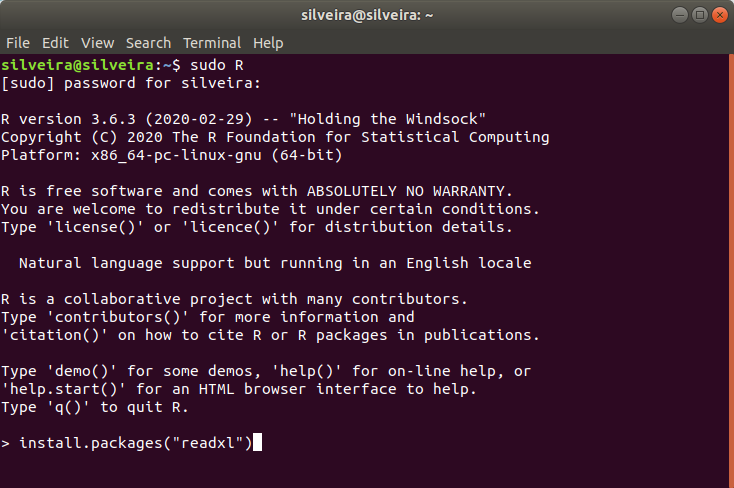
\includegraphics[width=0.9\linewidth]{R_installpackage} \end{center}

Um instalação, geralmente, escreve várias coisas no terminal, que o
instalador precisará ler \emph{\textbf{apenas no caso de algo dar
errado}}. Observe, principalmente, as últimas linhas. Caso termine com

{* DONE (readxl)}

sua instalação foi bem sucedida.

\begin{center}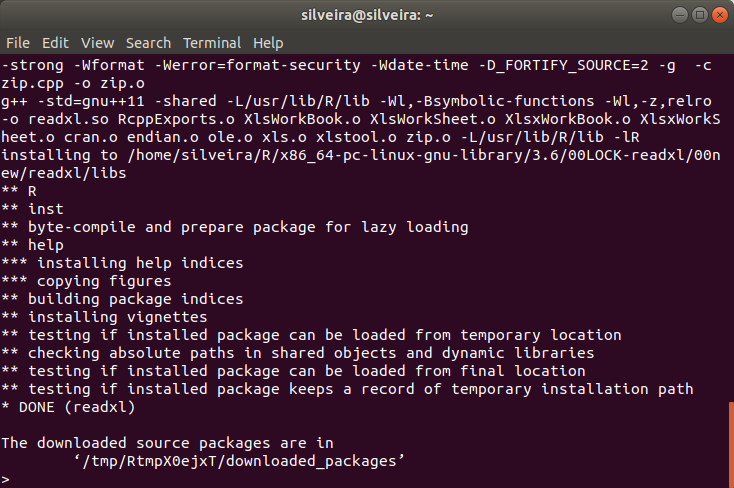
\includegraphics[width=0.9\linewidth]{R_installpackage2} \end{center}

\begin{center}\rule{0.5\linewidth}{0.5pt}\end{center}

\begin{center}\rule{0.5\linewidth}{0.5pt}\end{center}

\begin{flushleft}
\includegraphics[width=0.08\linewidth]{coruja} \end{flushleft}

O pacote eiras (disponível em
\url{https://github.com/pspsilveira/eiras}) ainda não está no CRAN. Para
instalá-lo, então, você precisará baixar do \textbf{github} o arquivo
que está na subpasta source\_package e, então, usar a linha de comando

\begin{quote}
install.packages(``\textbf{pathname}eiras\_X.X.X.tar.gz'')
\end{quote}

onde \textbf{pathname} é o caminho até a pasta onde você baixou o
arquivo e eiras\_X.X.X.tar.gz deve ser substituído pela versão mais
recente que estiver disponível. Por exemplo, no terminal Linux, tendo
baixado a versão 0.1.1. para uma pasta chamada tmp localizada na área de
trabalho de meu usuário, o comando é

\begin{quote}
install.packages(``/home/silveira/tmp/eiras\_0.1.1.tar.gz'')
\end{quote}

ou usar o auxílio do RStudio (Tools -\textgreater{} Install
packages\ldots), mudando do CRAN para um \emph{Package Archive File
(.tar.gz)} e apontando o arquivo para instalar.

\begin{center}\rule{0.5\linewidth}{0.5pt}\end{center}

\hypertarget{arquivos-em-outros-formatos}{%
\subsubsection{Arquivos em outros
formatos}\label{arquivos-em-outros-formatos}}

Há alguns outros formatos pré-instalados no RStudio. Funcionará como no
caso do Excel.

Por exemplo, para SPSS:

\begin{Shaded}
\begin{Highlighting}[]
\FunctionTok{library}\NormalTok{(haven)}
\NormalTok{dt\_anxproc1 }\OtherTok{\textless{}{-}}\NormalTok{ haven}\SpecialCharTok{::}\FunctionTok{read\_sav}\NormalTok{(}\StringTok{"AnxietyProcrastination.sav"}\NormalTok{)}
\end{Highlighting}
\end{Shaded}

Para Stata:

\begin{Shaded}
\begin{Highlighting}[]
\FunctionTok{library}\NormalTok{(haven)}
\NormalTok{lbw }\OtherTok{\textless{}{-}}\NormalTok{ haven}\SpecialCharTok{::}\FunctionTok{read\_dta}\NormalTok{(}\StringTok{"lbw.dta"}\NormalTok{)}
\end{Highlighting}
\end{Shaded}

Para o formato do LibreOffice (\emph{.ods}) não há nada pronto no
RStudio. Não é problema: existe \emph{package} para isto, como:

\begin{Shaded}
\begin{Highlighting}[]
\FunctionTok{library}\NormalTok{(readODS)}
\NormalTok{dt\_anxproc2 }\OtherTok{\textless{}{-}}\NormalTok{ readODS}\SpecialCharTok{::}\FunctionTok{read\_ods}\NormalTok{(}\StringTok{"AnxietyProcrastination.ods"}\NormalTok{)}
\end{Highlighting}
\end{Shaded}

Caso os execute serão criados \emph{data frames}, respectivamente
chamados dt\_anxproc1, lbw e dt\_anxproc2, todos com o mesmo conteúdo
(claramente, é preciso antes baixar os arquivos
\emph{\url{AnxietyProcrastination.sav}}, \emph{\url{lbw.dta}} e
\emph{\url{AnxietyProcrastination.ods}} para a pasta do projeto).

\begin{center}\rule{0.5\linewidth}{0.5pt}\end{center}

\begin{flushleft}
\includegraphics[width=0.08\linewidth]{coruja} \end{flushleft}

Estes dados também estão disponíveis no pacote eiras, disponível em
\url{https://github.com/pspsilveira/eiras} (em inglês).

A maneira de obtê-los depende do formato em que foram armazenados. No
formato padrão do R:

\begin{Shaded}
\begin{Highlighting}[]
\NormalTok{ctcp }\OtherTok{\textless{}{-}}\NormalTok{ eiras}\SpecialCharTok{::}\NormalTok{contraceptive}
\FunctionTok{print}\NormalTok{(ctcp)}

\NormalTok{procrastinacao }\OtherTok{\textless{}{-}}\NormalTok{ eiras}\SpecialCharTok{::}\NormalTok{procrastination}
\FunctionTok{print}\NormalTok{(procrastinacao)}

\NormalTok{lbw }\OtherTok{\textless{}{-}}\NormalTok{ eiras}\SpecialCharTok{::}\NormalTok{lbw}
\FunctionTok{print}\NormalTok{(lbw)}
\end{Highlighting}
\end{Shaded}

Nos outros formatos mencionados, a sintaxe é similar à dos exemplos
acima:

\begin{Shaded}
\begin{Highlighting}[]
\NormalTok{cm }\OtherTok{\textless{}{-}}\NormalTok{ readxl}\SpecialCharTok{::}\FunctionTok{read\_excel}\NormalTok{(}\FunctionTok{system.file}\NormalTok{(}\StringTok{"extdata"}\NormalTok{,}\StringTok{"contraceptive.xlsx"}\NormalTok{,}\AttributeTok{package=}\StringTok{"eiras"}\NormalTok{))}
\FunctionTok{print}\NormalTok{(cm)}

\NormalTok{anxproc }\OtherTok{\textless{}{-}}\NormalTok{ haven}\SpecialCharTok{::}\FunctionTok{read\_sav}\NormalTok{(}\FunctionTok{system.file}\NormalTok{(}\StringTok{"extdata"}\NormalTok{,}\StringTok{"procrastination.sav"}\NormalTok{,}\AttributeTok{package=}\StringTok{"eiras"}\NormalTok{))}
\FunctionTok{print}\NormalTok{(anxproc)}

\NormalTok{lbw }\OtherTok{\textless{}{-}}\NormalTok{ haven}\SpecialCharTok{::}\FunctionTok{read\_dta}\NormalTok{(}\FunctionTok{system.file}\NormalTok{(}\StringTok{"extdata"}\NormalTok{,}\StringTok{"lbw.dta"}\NormalTok{,}\AttributeTok{package=}\StringTok{"eiras"}\NormalTok{))}
\FunctionTok{print}\NormalTok{(lbw)}

\NormalTok{anxproc2 }\OtherTok{\textless{}{-}}\NormalTok{ readODS}\SpecialCharTok{::}\FunctionTok{read\_ods}\NormalTok{(}\FunctionTok{system.file}\NormalTok{(}\StringTok{"extdata"}\NormalTok{,}\StringTok{"procrastination.ods"}\NormalTok{,}\AttributeTok{package=}\StringTok{"eiras"}\NormalTok{))}
\FunctionTok{print}\NormalTok{(anxproc2)}
\end{Highlighting}
\end{Shaded}

\begin{center}\rule{0.5\linewidth}{0.5pt}\end{center}

\hypertarget{manipulando-um-data-frame}{%
\subsection{Manipulando um data frame}\label{manipulando-um-data-frame}}

\hypertarget{retomando-o-data-frame}{%
\subsubsection{\texorpdfstring{retomando o \emph{data
frame}}{retomando o data frame}}\label{retomando-o-data-frame}}

Vamos retormar o \emph{data frame} metodos com os seguintes comandos, já
executados:

\begin{Shaded}
\begin{Highlighting}[]
\FunctionTok{library}\NormalTok{(readxl)}
\NormalTok{metodos }\OtherTok{\textless{}{-}}\NormalTok{ readxl}\SpecialCharTok{::}\FunctionTok{read\_excel}\NormalTok{(}\StringTok{"MetodoAnticoncepcional.xlsx"}\NormalTok{)}
\FunctionTok{is.data.frame}\NormalTok{(metodos)}
\end{Highlighting}
\end{Shaded}

\begin{verbatim}
[1] TRUE
\end{verbatim}

\hypertarget{acessando-elementos-individuais-de-um-data-frame}{%
\subsubsection{\texorpdfstring{acessando elementos individuais de um
\emph{data
frame}}{acessando elementos individuais de um data frame}}\label{acessando-elementos-individuais-de-um-data-frame}}

Podemos verificar tanto o conteúdo das colunas de um \emph{data frame}
quanto os tipos de variável nele contidos.

O conteúdo das colunas podem ser acessados, fornecendo simplesmente o
nome da variável:

\begin{Shaded}
\begin{Highlighting}[]
\NormalTok{metodos}\SpecialCharTok{$}\NormalTok{Idade}
\end{Highlighting}
\end{Shaded}

\begin{verbatim}
 [1] 15 15 16 17 16 15 17 16 17 16 16 17 15 15 14 16 16 18 14 16 17 16 15 16 17
[26] 18 18 15 16 16 16 14 15 15 16 17 14 16 15 16 16 15 16 18 19 18 18 16 17 18
[51] 15 17 16 16 18 15 17 15 16 15
\end{verbatim}

Note o símbolo \$, significando que queremos a coluna Idade que está
dentro do \emph{data frame} metodos.

Os números entre colchetes à esquerda representam a posição do primeiro
elemento exibido em cada linha. Por exemplo, o primeiro elemento contém
o valor 15

\begin{Shaded}
\begin{Highlighting}[]
\NormalTok{metodos}\SpecialCharTok{$}\NormalTok{Idade[}\DecValTok{1}\NormalTok{]}
\end{Highlighting}
\end{Shaded}

\begin{verbatim}
[1] 15
\end{verbatim}

o vigésimo sexto elemento contém o valor 18:

\begin{Shaded}
\begin{Highlighting}[]
\NormalTok{metodos}\SpecialCharTok{$}\NormalTok{Idade[}\DecValTok{26}\NormalTok{]}
\end{Highlighting}
\end{Shaded}

\begin{verbatim}
[1] 18
\end{verbatim}

o quinquagésimo terceiro contém o valor 16:

\begin{Shaded}
\begin{Highlighting}[]
\NormalTok{metodos}\SpecialCharTok{$}\NormalTok{Idade[}\DecValTok{53}\NormalTok{]}
\end{Highlighting}
\end{Shaded}

\begin{verbatim}
[1] 16
\end{verbatim}

e o último elemento contém o valor 15:

\begin{Shaded}
\begin{Highlighting}[]
\NormalTok{metodos}\SpecialCharTok{$}\NormalTok{Idade[}\DecValTok{60}\NormalTok{]}
\end{Highlighting}
\end{Shaded}

\begin{verbatim}
[1] 15
\end{verbatim}

\begin{center}\rule{0.5\linewidth}{0.5pt}\end{center}

\begin{flushleft}
\includegraphics[width=0.08\linewidth]{coruja} \end{flushleft}

Em situações em que o número de linhas (\emph{rows}, em inglês) não é
conhecido, o último elemento pode ser acessado com:

\begin{Shaded}
\begin{Highlighting}[]
\NormalTok{metodos}\SpecialCharTok{$}\NormalTok{Idade[}\FunctionTok{nrow}\NormalTok{(metodos)]}
\end{Highlighting}
\end{Shaded}

\begin{verbatim}
[1] 15
\end{verbatim}

A função nrow(), aninhada dentros dos colchetes, devolve o número de
linhas que metodos tem; neste caso:

\begin{Shaded}
\begin{Highlighting}[]
\FunctionTok{nrow}\NormalTok{(metodos)}
\end{Highlighting}
\end{Shaded}

\begin{verbatim}
[1] 60
\end{verbatim}

devolve o valor 60.

Note que o R executa os colchetes e parênteses em uma expressão do mais
interno para fora. Então, metodos\$Idade{[}nrow(metodos){]} torna-se
metodos\$Idade{[}60{]} e esta variável contém o valor 15.

\begin{center}\rule{0.5\linewidth}{0.5pt}\end{center}

Os elementos da coluna metodos\$Idade são todos números:

\begin{Shaded}
\begin{Highlighting}[]
\FunctionTok{is.numeric}\NormalTok{(metodos}\SpecialCharTok{$}\NormalTok{Idade)}
\end{Highlighting}
\end{Shaded}

\begin{verbatim}
[1] TRUE
\end{verbatim}

E podemos perguntar se são, por exemplo, finitos (e, neste caso, cada
valor é verificado):

\begin{Shaded}
\begin{Highlighting}[]
\FunctionTok{is.finite}\NormalTok{(metodos}\SpecialCharTok{$}\NormalTok{Idade)}
\end{Highlighting}
\end{Shaded}

\begin{verbatim}
 [1] TRUE TRUE TRUE TRUE TRUE TRUE TRUE TRUE TRUE TRUE TRUE TRUE TRUE TRUE TRUE
[16] TRUE TRUE TRUE TRUE TRUE TRUE TRUE TRUE TRUE TRUE TRUE TRUE TRUE TRUE TRUE
[31] TRUE TRUE TRUE TRUE TRUE TRUE TRUE TRUE TRUE TRUE TRUE TRUE TRUE TRUE TRUE
[46] TRUE TRUE TRUE TRUE TRUE TRUE TRUE TRUE TRUE TRUE TRUE TRUE TRUE TRUE TRUE
\end{verbatim}

\begin{center}\rule{0.5\linewidth}{0.5pt}\end{center}

\begin{flushleft}
\includegraphics[width=0.08\linewidth]{coruja} \end{flushleft}

Em conexão com o comentário, acima, de que em R há muitos tipos de
variáveis que não têm correspondência em outras linguagens de
programação, note também que uma variável pode ser vista como se tivesse
vários ``tipos'' e ou ``subtipos'' simultaneamente. Por exemplo, a
coluna Idade, além de numérica e contendo números finitos, também pode
ser tratada como um vetor.

\begin{Shaded}
\begin{Highlighting}[]
\FunctionTok{is.vector}\NormalTok{(metodos}\SpecialCharTok{$}\NormalTok{Idade)}
\end{Highlighting}
\end{Shaded}

\begin{verbatim}
[1] TRUE
\end{verbatim}

\begin{center}\rule{0.5\linewidth}{0.5pt}\end{center}

A coluna Metodo, obviamente, não é numérica:

\begin{Shaded}
\begin{Highlighting}[]
\FunctionTok{is.numeric}\NormalTok{(metodos}\SpecialCharTok{$}\NormalTok{Metodo)}
\end{Highlighting}
\end{Shaded}

\begin{verbatim}
[1] FALSE
\end{verbatim}

\begin{center}\rule{0.5\linewidth}{0.5pt}\end{center}

\begin{flushleft}
\includegraphics[width=0.08\linewidth]{coruja} \end{flushleft}

Não confunda metodos, que é o nome que demos ao \emph{data frame}, com
Metodo que é uma coluna do \emph{data frame}, a qual é endereçada por
metodos\$Metodo.

\begin{center}\rule{0.5\linewidth}{0.5pt}\end{center}

A coluna metodos\$Metodo poderia ser um fator, uma vez que tem poucos
valores diferentes:

\begin{Shaded}
\begin{Highlighting}[]
\FunctionTok{unique}\NormalTok{(metodos}\SpecialCharTok{$}\NormalTok{Metodo)}
\end{Highlighting}
\end{Shaded}

\begin{verbatim}
[1] "Tabelinha"    "Preservativo" "Pílula"       "Outro"       
\end{verbatim}

No entanto, a função read\_excel a trouxe como uma variável
\emph{character}:

\begin{Shaded}
\begin{Highlighting}[]
\FunctionTok{is.factor}\NormalTok{(metodos}\SpecialCharTok{$}\NormalTok{Metodo)}
\end{Highlighting}
\end{Shaded}

\begin{verbatim}
[1] FALSE
\end{verbatim}

\begin{Shaded}
\begin{Highlighting}[]
\FunctionTok{is.character}\NormalTok{(metodos}\SpecialCharTok{$}\NormalTok{Metodo)}
\end{Highlighting}
\end{Shaded}

\begin{verbatim}
[1] TRUE
\end{verbatim}

Isto pode ser corrigido; voltaremos a lidar com fatores adiante.

\emph{Data frames} são organizados em {[}linha,coluna{]}. É possível
acessar uma linha específica de um \emph{data frame} pelo seu número. A
segunda linha contém:

\begin{Shaded}
\begin{Highlighting}[]
\NormalTok{metodos[}\DecValTok{2}\NormalTok{,]}
\end{Highlighting}
\end{Shaded}

\begin{verbatim}
# A tibble: 1 x 3
     ID Idade Metodo   
  <dbl> <dbl> <chr>    
1     2    15 Tabelinha
\end{verbatim}

Podemos também acessar uma coluna pelo seu número. A terceira coluna
contém:

\begin{Shaded}
\begin{Highlighting}[]
\NormalTok{metodos[,}\DecValTok{3}\NormalTok{]}
\end{Highlighting}
\end{Shaded}

\begin{verbatim}
# A tibble: 60 x 1
   Metodo      
   <chr>       
 1 Tabelinha   
 2 Tabelinha   
 3 Preservativo
 4 Pílula      
 5 Pílula      
 6 Tabelinha   
 7 Tabelinha   
 8 Preservativo
 9 Pílula      
10 Preservativo
# ... with 50 more rows
\end{verbatim}

o mesmo que buscar por

\begin{Shaded}
\begin{Highlighting}[]
\NormalTok{metodos[, }\StringTok{"Metodo"}\NormalTok{]}
\end{Highlighting}
\end{Shaded}

\begin{verbatim}
# A tibble: 60 x 1
   Metodo      
   <chr>       
 1 Tabelinha   
 2 Tabelinha   
 3 Preservativo
 4 Pílula      
 5 Pílula      
 6 Tabelinha   
 7 Tabelinha   
 8 Preservativo
 9 Pílula      
10 Preservativo
# ... with 50 more rows
\end{verbatim}

Podemos combinar linha e coluna. O conteúdo da segunda linha, terceira
coluna contém:

\begin{Shaded}
\begin{Highlighting}[]
\NormalTok{metodos[}\DecValTok{2}\NormalTok{,}\DecValTok{3}\NormalTok{]}
\end{Highlighting}
\end{Shaded}

\begin{verbatim}
# A tibble: 1 x 1
  Metodo   
  <chr>    
1 Tabelinha
\end{verbatim}

\begin{center}\rule{0.5\linewidth}{0.5pt}\end{center}

\begin{flushleft}
\includegraphics[width=0.08\linewidth]{coruja} \end{flushleft}

A coluna Idade é a segunda coluna do \emph{data frame}. Antes, acessamos
esta coluna com

\begin{Shaded}
\begin{Highlighting}[]
\NormalTok{metodos}\SpecialCharTok{$}\NormalTok{Idade}
\end{Highlighting}
\end{Shaded}

\begin{verbatim}
 [1] 15 15 16 17 16 15 17 16 17 16 16 17 15 15 14 16 16 18 14 16 17 16 15 16 17
[26] 18 18 15 16 16 16 14 15 15 16 17 14 16 15 16 16 15 16 18 19 18 18 16 17 18
[51] 15 17 16 16 18 15 17 15 16 15
\end{verbatim}

e vimos que R nos fornece um vetor numérico. Podemos acessar os dados
também pelo número da coluna com

\begin{Shaded}
\begin{Highlighting}[]
\NormalTok{metodos[,}\DecValTok{2}\NormalTok{]}
\end{Highlighting}
\end{Shaded}

\begin{verbatim}
# A tibble: 60 x 1
   Idade
   <dbl>
 1    15
 2    15
 3    16
 4    17
 5    16
 6    15
 7    17
 8    16
 9    17
10    16
# ... with 50 more rows
\end{verbatim}

Observe que os dados são os mesmos, mas o formato não é. Acessando pelo
número da coluna não obtivemos um vetor numérico. Caso precise, por
exemplo para que uma função que aguarde dados neste formato, o
equivalente é:

\begin{Shaded}
\begin{Highlighting}[]
\FunctionTok{as.numeric}\NormalTok{(}\FunctionTok{unlist}\NormalTok{(metodos[,}\DecValTok{2}\NormalTok{]))}
\end{Highlighting}
\end{Shaded}

\begin{verbatim}
 [1] 15 15 16 17 16 15 17 16 17 16 16 17 15 15 14 16 16 18 14 16 17 16 15 16 17
[26] 18 18 15 16 16 16 14 15 15 16 17 14 16 15 16 16 15 16 18 19 18 18 16 17 18
[51] 15 17 16 16 18 15 17 15 16 15
\end{verbatim}

ou

\begin{Shaded}
\begin{Highlighting}[]
\FunctionTok{as.numeric}\NormalTok{(}\FunctionTok{unlist}\NormalTok{(metodos[}\StringTok{"Idade"}\NormalTok{]))}
\end{Highlighting}
\end{Shaded}

\begin{verbatim}
 [1] 15 15 16 17 16 15 17 16 17 16 16 17 15 15 14 16 16 18 14 16 17 16 15 16 17
[26] 18 18 15 16 16 16 14 15 15 16 17 14 16 15 16 16 15 16 18 19 18 18 16 17 18
[51] 15 17 16 16 18 15 17 15 16 15
\end{verbatim}

Caso queiramos os métodos em um vetor alfanumérico, pode usar (pelo
número da coluna ou pelo nome da coluna) algo como:

\begin{Shaded}
\begin{Highlighting}[]
\FunctionTok{as.character}\NormalTok{(}\FunctionTok{unlist}\NormalTok{(metodos[}\StringTok{"Metodo"}\NormalTok{]))}
\end{Highlighting}
\end{Shaded}

\begin{verbatim}
 [1] "Tabelinha"    "Tabelinha"    "Preservativo" "Pílula"       "Pílula"      
 [6] "Tabelinha"    "Tabelinha"    "Preservativo" "Pílula"       "Preservativo"
[11] "Preservativo" "Preservativo" "Outro"        "Pílula"       "Preservativo"
[16] "Tabelinha"    "Tabelinha"    "Outro"        "Pílula"       "Outro"       
[21] "Preservativo" "Pílula"       "Tabelinha"    "Tabelinha"    "Tabelinha"   
[26] "Pílula"       "Tabelinha"    "Preservativo" "Preservativo" "Tabelinha"   
[31] "Outro"        "Tabelinha"    "Tabelinha"    "Preservativo" "Pílula"      
[36] "Pílula"       "Preservativo" "Preservativo" "Preservativo" "Outro"       
[41] "Tabelinha"    "Tabelinha"    "Pílula"       "Tabelinha"    "Pílula"      
[46] "Preservativo" "Preservativo" "Tabelinha"    "Preservativo" "Pílula"      
[51] "Tabelinha"    "Tabelinha"    "Preservativo" "Preservativo" "Pílula"      
[56] "Tabelinha"    "Tabelinha"    "Pílula"       "Preservativo" "Tabelinha"   
\end{verbatim}

\begin{center}\rule{0.5\linewidth}{0.5pt}\end{center}

\hypertarget{selecionando-dados}{%
\subsubsection{selecionando dados}\label{selecionando-dados}}

É possível filtrar por determinadas condições. Existem operadores:

\begin{itemize}
\tightlist
\item
  de comparação: \textless{} (menor), \textless= (menor ou igual), ==
  (igual), != (diferente), \textgreater= (maior ou igual) e
  \textgreater{} (maior).
\item
  lógicos: \& (\emph{and}), \textbar{} (\emph{or}) e ! (\emph{not}).
\end{itemize}

As linhas dos indivíduos com idade menor ou igual a 15 anos são:

\begin{Shaded}
\begin{Highlighting}[]
\NormalTok{dftmp }\OtherTok{\textless{}{-}}\NormalTok{ metodos[metodos}\SpecialCharTok{$}\NormalTok{Idade}\SpecialCharTok{\textless{}=}\DecValTok{15}\NormalTok{,]}
\FunctionTok{print}\NormalTok{(dftmp)}
\end{Highlighting}
\end{Shaded}

\begin{verbatim}
# A tibble: 19 x 3
      ID Idade Metodo      
   <dbl> <dbl> <chr>       
 1     1    15 Tabelinha   
 2     2    15 Tabelinha   
 3     6    15 Tabelinha   
 4    13    15 Outro       
 5    14    15 Pílula      
 6    15    14 Preservativo
 7    19    14 Pílula      
 8    23    15 Tabelinha   
 9    28    15 Preservativo
10    32    14 Tabelinha   
11    33    15 Tabelinha   
12    34    15 Preservativo
13    37    14 Preservativo
14    39    15 Preservativo
15    42    15 Tabelinha   
16    51    15 Tabelinha   
17    56    15 Tabelinha   
18    58    15 Pílula      
19    60    15 Tabelinha   
\end{verbatim}

Este dftmp é um \emph{data frame}, contendo um subconjunto de metodos.
Caso não apareça inteiro na \emph{Console} (print() só exibe as
primeiras linhas), use a aba \emph{Environment} para ver todo o seu
conteúdo e confira o sucesso desta operação.

Quem não tem 17 é dado por:

\begin{Shaded}
\begin{Highlighting}[]
\NormalTok{dftmp }\OtherTok{\textless{}{-}}\NormalTok{ metodos[metodos}\SpecialCharTok{$}\NormalTok{Idade}\SpecialCharTok{!=}\DecValTok{17}\NormalTok{,]}
\FunctionTok{print}\NormalTok{(dftmp)}
\end{Highlighting}
\end{Shaded}

\begin{verbatim}
# A tibble: 50 x 3
      ID Idade Metodo      
   <dbl> <dbl> <chr>       
 1     1    15 Tabelinha   
 2     2    15 Tabelinha   
 3     3    16 Preservativo
 4     5    16 Pílula      
 5     6    15 Tabelinha   
 6     8    16 Preservativo
 7    10    16 Preservativo
 8    11    16 Preservativo
 9    13    15 Outro       
10    14    15 Pílula      
# ... with 40 more rows
\end{verbatim}

Por exemplo, para saber quais estão entre 15 \textbf{e} 18 anos de idade
(incluindo 15 mas não incluindo 18):

\begin{Shaded}
\begin{Highlighting}[]
\NormalTok{dftmp }\OtherTok{\textless{}{-}}\NormalTok{ metodos[metodos}\SpecialCharTok{$}\NormalTok{Idade}\SpecialCharTok{\textgreater{}=}\DecValTok{15} \SpecialCharTok{\&}\NormalTok{ metodos}\SpecialCharTok{$}\NormalTok{Idade}\SpecialCharTok{\textless{}}\DecValTok{18}\NormalTok{,]}
\FunctionTok{print}\NormalTok{(dftmp)}
\end{Highlighting}
\end{Shaded}

\begin{verbatim}
# A tibble: 47 x 3
      ID Idade Metodo      
   <dbl> <dbl> <chr>       
 1     1    15 Tabelinha   
 2     2    15 Tabelinha   
 3     3    16 Preservativo
 4     4    17 Pílula      
 5     5    16 Pílula      
 6     6    15 Tabelinha   
 7     7    17 Tabelinha   
 8     8    16 Preservativo
 9     9    17 Pílula      
10    10    16 Preservativo
# ... with 37 more rows
\end{verbatim}

Para saber quem tem menos que 15 (inclusive) \textbf{ou} exatamente 17:

\begin{Shaded}
\begin{Highlighting}[]
\NormalTok{dftmp }\OtherTok{\textless{}{-}}\NormalTok{ metodos[metodos}\SpecialCharTok{$}\NormalTok{Idade}\SpecialCharTok{\textless{}=}\DecValTok{15} \SpecialCharTok{|}\NormalTok{ metodos}\SpecialCharTok{$}\NormalTok{Idade}\SpecialCharTok{==}\DecValTok{17}\NormalTok{,]}
\FunctionTok{print}\NormalTok{(dftmp)}
\end{Highlighting}
\end{Shaded}

\begin{verbatim}
# A tibble: 29 x 3
      ID Idade Metodo      
   <dbl> <dbl> <chr>       
 1     1    15 Tabelinha   
 2     2    15 Tabelinha   
 3     4    17 Pílula      
 4     6    15 Tabelinha   
 5     7    17 Tabelinha   
 6     9    17 Pílula      
 7    12    17 Preservativo
 8    13    15 Outro       
 9    14    15 Pílula      
10    15    14 Preservativo
# ... with 19 more rows
\end{verbatim}

Para saber quem não é menor de idade (i.e., idades que não são menores
que 18 anos), precisamos saber quem tem menor que 17 ou, pela negativa,
quem não tem mais que 18:

\begin{Shaded}
\begin{Highlighting}[]
\NormalTok{dftmp }\OtherTok{\textless{}{-}}\NormalTok{ metodos[metodos}\SpecialCharTok{$}\NormalTok{Idade}\SpecialCharTok{\textless{}=}\DecValTok{17}\NormalTok{,]}
\FunctionTok{print}\NormalTok{(dftmp)}
\end{Highlighting}
\end{Shaded}

\begin{verbatim}
# A tibble: 51 x 3
      ID Idade Metodo      
   <dbl> <dbl> <chr>       
 1     1    15 Tabelinha   
 2     2    15 Tabelinha   
 3     3    16 Preservativo
 4     4    17 Pílula      
 5     5    16 Pílula      
 6     6    15 Tabelinha   
 7     7    17 Tabelinha   
 8     8    16 Preservativo
 9     9    17 Pílula      
10    10    16 Preservativo
# ... with 41 more rows
\end{verbatim}

ou

\begin{Shaded}
\begin{Highlighting}[]
\NormalTok{dftmp }\OtherTok{\textless{}{-}}\NormalTok{ metodos[}\SpecialCharTok{!}\NormalTok{metodos}\SpecialCharTok{$}\NormalTok{Idade}\SpecialCharTok{\textgreater{}=}\DecValTok{18}\NormalTok{,]}
\FunctionTok{print}\NormalTok{(dftmp)}
\end{Highlighting}
\end{Shaded}

\begin{verbatim}
# A tibble: 51 x 3
      ID Idade Metodo      
   <dbl> <dbl> <chr>       
 1     1    15 Tabelinha   
 2     2    15 Tabelinha   
 3     3    16 Preservativo
 4     4    17 Pílula      
 5     5    16 Pílula      
 6     6    15 Tabelinha   
 7     7    17 Tabelinha   
 8     8    16 Preservativo
 9     9    17 Pílula      
10    10    16 Preservativo
# ... with 41 more rows
\end{verbatim}

Os operadores podem ser combinados. A ordem das comparações é dada por
(), indo do mais interno para o mais externo, se forem aninhados. Por
exemplo, os cálculos são diferentes:

\begin{Shaded}
\begin{Highlighting}[]
  \DecValTok{1}\SpecialCharTok{+}\DecValTok{3} \SpecialCharTok{/} \DecValTok{4}\SpecialCharTok{+}\DecValTok{5} \SpecialCharTok{/} \DecValTok{2}
\end{Highlighting}
\end{Shaded}

\begin{verbatim}
[1] 4.25
\end{verbatim}

\begin{Shaded}
\begin{Highlighting}[]
\NormalTok{((}\DecValTok{1}\SpecialCharTok{+}\DecValTok{3}\NormalTok{)}\SpecialCharTok{/}\NormalTok{(}\DecValTok{4}\SpecialCharTok{+}\DecValTok{5}\NormalTok{)) }\SpecialCharTok{/} \DecValTok{2}
\end{Highlighting}
\end{Shaded}

\begin{verbatim}
[1] 0.2222222
\end{verbatim}

O primeiro obedece a precedência habitual da matemática (divisão vem
antes da soma). Então divide 3 por 4 resultando em 0.75, então 5 por 2
resultando em 2.5, e finalmente faz a soma de 1+0.75+2.5 resultando em
4.25; se não era o pretendido, os espaços em branco nada resolvem (são
ignorados). O segundo soma 1+3 (resulta em 4), depois 3+5 (resulta em
8), então divide 4 por 8 resultando em 0.5 e, finalmente, divide por 2
resultando em 0.25. Na dúvida sobre a precedência das operações, use e
abuse dos ().

Da mesma forma, para comparações a ordem é regulada com (). Se quisermos
saber quem tem entre (15 \textbf{e} 16) \textbf{ou} entre (18 \textbf{e}
19), inclusive

\begin{Shaded}
\begin{Highlighting}[]
\NormalTok{dftmp }\OtherTok{\textless{}{-}}\NormalTok{ metodos[(metodos}\SpecialCharTok{$}\NormalTok{Idade}\SpecialCharTok{\textgreater{}=}\DecValTok{15} \SpecialCharTok{\&}\NormalTok{ metodos}\SpecialCharTok{$}\NormalTok{Idade}\SpecialCharTok{\textless{}=}\DecValTok{16}\NormalTok{) }\SpecialCharTok{|} 
\NormalTok{                 (metodos}\SpecialCharTok{$}\NormalTok{Idade}\SpecialCharTok{\textgreater{}=}\DecValTok{18} \SpecialCharTok{\&}\NormalTok{ metodos}\SpecialCharTok{$}\NormalTok{Idade}\SpecialCharTok{\textless{}=}\DecValTok{19}\NormalTok{),]}
\FunctionTok{print}\NormalTok{(dftmp)}
\end{Highlighting}
\end{Shaded}

\begin{verbatim}
# A tibble: 46 x 3
      ID Idade Metodo      
   <dbl> <dbl> <chr>       
 1     1    15 Tabelinha   
 2     2    15 Tabelinha   
 3     3    16 Preservativo
 4     5    16 Pílula      
 5     6    15 Tabelinha   
 6     8    16 Preservativo
 7    10    16 Preservativo
 8    11    16 Preservativo
 9    13    15 Outro       
10    14    15 Pílula      
# ... with 36 more rows
\end{verbatim}

(a linha quebrada após \textbar{} é opcional; apenas para facilitar a
legibilidade do código, evitando escrever linhas muito longas que saem
da tela).

\hypertarget{alterando-o-conteuxfado-do-data-frame}{%
\subsubsection{alterando o conteúdo do data
frame}\label{alterando-o-conteuxfado-do-data-frame}}

Como podemos acessar os elementos de um \emph{data frame}, podemos
também alterar seus valores usando o operador de atribuição, \textless-.
Por exemplo:

\begin{Shaded}
\begin{Highlighting}[]
\NormalTok{metodos}\SpecialCharTok{$}\NormalTok{Idade[}\DecValTok{45}\NormalTok{] }\OtherTok{\textless{}{-}} \FloatTok{19.5}
\end{Highlighting}
\end{Shaded}

e confira com

\begin{Shaded}
\begin{Highlighting}[]
\NormalTok{metodos}\SpecialCharTok{$}\NormalTok{Idade}
\end{Highlighting}
\end{Shaded}

\begin{verbatim}
 [1] 15.0 15.0 16.0 17.0 16.0 15.0 17.0 16.0 17.0 16.0 16.0 17.0 15.0 15.0 14.0
[16] 16.0 16.0 18.0 14.0 16.0 17.0 16.0 15.0 16.0 17.0 18.0 18.0 15.0 16.0 16.0
[31] 16.0 14.0 15.0 15.0 16.0 17.0 14.0 16.0 15.0 16.0 16.0 15.0 16.0 18.0 19.5
[46] 18.0 18.0 16.0 17.0 18.0 15.0 17.0 16.0 16.0 18.0 15.0 17.0 15.0 16.0 15.0
\end{verbatim}

(localize o 450 elemento e veja que seu valor é, agora, 19.5).

Mais uma coisa aconteceu. Notou que, ao adicionarmos um elemento com uma
casa decimal, todos os valores agora apareceram com uma casa decimal? Um
vetor tem que ter elementos todos do mesmo tipo e, para acomodar o 19.5,
é inteiramente formado por números do tipo \emph{double} (a forma do R
dizer que é número fracionário).

\begin{Shaded}
\begin{Highlighting}[]
\FunctionTok{is.numeric}\NormalTok{(metodos}\SpecialCharTok{$}\NormalTok{Idade)}
\end{Highlighting}
\end{Shaded}

\begin{verbatim}
[1] TRUE
\end{verbatim}

\begin{Shaded}
\begin{Highlighting}[]
\FunctionTok{is.integer}\NormalTok{(metodos}\SpecialCharTok{$}\NormalTok{Idade)}
\end{Highlighting}
\end{Shaded}

\begin{verbatim}
[1] FALSE
\end{verbatim}

\begin{Shaded}
\begin{Highlighting}[]
\FunctionTok{is.double}\NormalTok{(metodos}\SpecialCharTok{$}\NormalTok{Idade)}
\end{Highlighting}
\end{Shaded}

\begin{verbatim}
[1] TRUE
\end{verbatim}

A esta altura você pode imaginar que devem existir muitas funções R
iniciadas com is\ldots() e que pode ser uma tarefa insana ficar tentando
várias funções até adivinhar com qual tipo estamos lidando. Podemos
reproduzir na \emph{Console} as informações de uma variável que aparecem
na aba \emph{Environment} com a função str() (de \emph{structure},
estrutura):

\begin{Shaded}
\begin{Highlighting}[]
\FunctionTok{str}\NormalTok{(metodos)}
\end{Highlighting}
\end{Shaded}

\begin{verbatim}
tibble [60 x 3] (S3: tbl_df/tbl/data.frame)
 $ ID    : num [1:60] 1 2 3 4 5 6 7 8 9 10 ...
 $ Idade : num [1:60] 15 15 16 17 16 15 17 16 17 16 ...
 $ Metodo: chr [1:60] "Tabelinha" "Tabelinha" "Preservativo" "Pílula" ...
\end{verbatim}

mostrando a coluna ID é numérica (\emph{num}), Idade é numérica e Metodo
é character (\emph{chr}).

Ajuda, ainda, conhecer a função \emph{sapply()}:

\begin{Shaded}
\begin{Highlighting}[]
\FunctionTok{sapply}\NormalTok{(metodos, typeof)}
\end{Highlighting}
\end{Shaded}

\begin{verbatim}
         ID       Idade      Metodo 
   "double"    "double" "character" 
\end{verbatim}

que informa o tipo \emph{double} para metodos\$Idade.

\begin{center}\rule{0.5\linewidth}{0.5pt}\end{center}

\begin{flushleft}
\includegraphics[width=0.08\linewidth]{coruja} \end{flushleft}

Como sempre, se usamos apenas o nome da variável metodos na
\emph{Console}, R tenta exibir todo seu conteúdo:

\begin{Shaded}
\begin{Highlighting}[]
\NormalTok{metodos}
\end{Highlighting}
\end{Shaded}

\begin{verbatim}
# A tibble: 60 x 3
      ID Idade Metodo      
   <dbl> <dbl> <chr>       
 1     1    15 Tabelinha   
 2     2    15 Tabelinha   
 3     3    16 Preservativo
 4     4    17 Pílula      
 5     5    16 Pílula      
 6     6    15 Tabelinha   
 7     7    17 Tabelinha   
 8     8    16 Preservativo
 9     9    17 Pílula      
10    10    16 Preservativo
# ... with 50 more rows
\end{verbatim}

Como são muitas linhas, R trunca e informa quantas não exibiu. Tentar
mostrar um \emph{data frame} desta forma, portanto, não é muito prático;
usar o ambiente do RStudio através da aba \emph{Environment} é muito
mais fácil.

Note, ainda, os números das linhas à esquerda. Estes são os números de
linha de metodos. Neste caso é apenas uma coincidência que sejam iguais
a metodos\$ID, pois os pacientes foram numerados sequencialmente no
arquivo original.

\begin{center}\rule{0.5\linewidth}{0.5pt}\end{center}

\hypertarget{alterando-o-tipo-de-variuxe1vel}{%
\subsubsection{alterando o tipo de
variável}\label{alterando-o-tipo-de-variuxe1vel}}

Caso lhe incomode que metodos\$ID seja um número, um tipo pode ser
convertido em outro:

\begin{Shaded}
\begin{Highlighting}[]
\NormalTok{metodos}\SpecialCharTok{$}\NormalTok{ID }\OtherTok{\textless{}{-}} \FunctionTok{as.character}\NormalTok{(metodos}\SpecialCharTok{$}\NormalTok{ID)}
\end{Highlighting}
\end{Shaded}

Repare que a função é as.character, significando \textbf{como
alfanumérica} (e não is.character(), que pergunta se \textbf{é
alfanumérica?}). Variáveis do tipo \emph{chr} são as que podem acomodar
textos como ``Tabelinha'', ``Outros métodos'' ou mesmo letras e números
combinados, como ``RG 123456''.

Também pode ser estranho atribuir a metodos\$ID uma operação feita com a
própria variável. O que acontece em linguagens de programação é que o
que está além do operador de atribuição \textless- é processado primeiro
e, então seu resultado é jogado na variável à sua esquerda. Neste
exemplo, o conteúdo de metodos\$ID é passado à função as.character, que
a devolve convertida em caracteres; o resultado desta operação é
atribuído à própria metodos\$ID, sobrepondo seus valores anteriores.
Confira que o tipo da variável metodos\$ID mudou para \emph{chr}:

\begin{Shaded}
\begin{Highlighting}[]
\FunctionTok{str}\NormalTok{(metodos)}
\end{Highlighting}
\end{Shaded}

\begin{verbatim}
tibble [60 x 3] (S3: tbl_df/tbl/data.frame)
 $ ID    : chr [1:60] "1" "2" "3" "4" ...
 $ Idade : num [1:60] 15 15 16 17 16 15 17 16 17 16 ...
 $ Metodo: chr [1:60] "Tabelinha" "Tabelinha" "Preservativo" "Pílula" ...
\end{verbatim}

\begin{center}\rule{0.5\linewidth}{0.5pt}\end{center}

Mencionamos, acima, que metodos\$Metodo deveria ser tratado como um
fator. Existe função para isto:

\begin{Shaded}
\begin{Highlighting}[]
\NormalTok{metodos}\SpecialCharTok{$}\NormalTok{Metodo }\OtherTok{\textless{}{-}} \FunctionTok{as.factor}\NormalTok{(metodos}\SpecialCharTok{$}\NormalTok{Metodo)}
\end{Highlighting}
\end{Shaded}

Confira que ocorreu com metodos\$Metodo:

\begin{Shaded}
\begin{Highlighting}[]
\FunctionTok{str}\NormalTok{(metodos)}
\end{Highlighting}
\end{Shaded}

\begin{verbatim}
tibble [60 x 3] (S3: tbl_df/tbl/data.frame)
 $ ID    : chr [1:60] "1" "2" "3" "4" ...
 $ Idade : num [1:60] 15 15 16 17 16 15 17 16 17 16 ...
 $ Metodo: Factor w/ 4 levels "Outro","Pílula",..: 4 4 3 2 2 4 4 3 2 3 ...
\end{verbatim}

Observe que metodos\$Metodo, sendo um fator (portanto uma variável
nominal), tem indicação de quantos níveis (i.e., quantos valores
diferentes existem) armazenados na variável. São 4, diferentes, como já
tínhamos visto com

\begin{Shaded}
\begin{Highlighting}[]
\FunctionTok{unique}\NormalTok{(metodos}\SpecialCharTok{$}\NormalTok{Metodo)}
\end{Highlighting}
\end{Shaded}

\begin{verbatim}
[1] Tabelinha    Preservativo Pílula       Outro       
Levels: Outro Pílula Preservativo Tabelinha
\end{verbatim}

Note também que os níveis têm números inteiros associados com cada
categoria. A ordem dos níveis do fator segue a ordem de aparição dos
dados no \emph{data frame}.

\begin{Shaded}
\begin{Highlighting}[]
\FunctionTok{print}\NormalTok{(metodos}\SpecialCharTok{$}\NormalTok{Metodo)}
\end{Highlighting}
\end{Shaded}

\begin{verbatim}
 [1] Tabelinha    Tabelinha    Preservativo Pílula       Pílula      
 [6] Tabelinha    Tabelinha    Preservativo Pílula       Preservativo
[11] Preservativo Preservativo Outro        Pílula       Preservativo
[16] Tabelinha    Tabelinha    Outro        Pílula       Outro       
[21] Preservativo Pílula       Tabelinha    Tabelinha    Tabelinha   
[26] Pílula       Tabelinha    Preservativo Preservativo Tabelinha   
[31] Outro        Tabelinha    Tabelinha    Preservativo Pílula      
[36] Pílula       Preservativo Preservativo Preservativo Outro       
[41] Tabelinha    Tabelinha    Pílula       Tabelinha    Pílula      
[46] Preservativo Preservativo Tabelinha    Preservativo Pílula      
[51] Tabelinha    Tabelinha    Preservativo Preservativo Pílula      
[56] Tabelinha    Tabelinha    Pílula       Preservativo Tabelinha   
Levels: Outro Pílula Preservativo Tabelinha
\end{verbatim}

Esta ordem, quando não é conveniente, pode ser escolhida com:

\begin{Shaded}
\begin{Highlighting}[]
\NormalTok{metodos}\SpecialCharTok{$}\NormalTok{Metodo }\OtherTok{\textless{}{-}} \FunctionTok{factor}\NormalTok{(metodos}\SpecialCharTok{$}\NormalTok{Metodo,}\AttributeTok{levels=}\FunctionTok{c}\NormalTok{(}\StringTok{"Tabelinha"}\NormalTok{,}\StringTok{"Pílula"}\NormalTok{,}\StringTok{"Preservativo"}\NormalTok{,}\StringTok{"Outro"}\NormalTok{))}
\end{Highlighting}
\end{Shaded}

Veja o que mudou com

\begin{Shaded}
\begin{Highlighting}[]
\FunctionTok{str}\NormalTok{(metodos)}
\end{Highlighting}
\end{Shaded}

\begin{verbatim}
tibble [60 x 3] (S3: tbl_df/tbl/data.frame)
 $ ID    : chr [1:60] "1" "2" "3" "4" ...
 $ Idade : num [1:60] 15 15 16 17 16 15 17 16 17 16 ...
 $ Metodo: Factor w/ 4 levels "Tabelinha","Pílula",..: 1 1 3 2 2 1 1 3 2 3 ...
\end{verbatim}

\begin{Shaded}
\begin{Highlighting}[]
\FunctionTok{unique}\NormalTok{(metodos}\SpecialCharTok{$}\NormalTok{Metodo)}
\end{Highlighting}
\end{Shaded}

\begin{verbatim}
[1] Tabelinha    Preservativo Pílula       Outro       
Levels: Tabelinha Pílula Preservativo Outro
\end{verbatim}

e observe a ordem dos \emph{levels} que a função unique() agora exibe.

\hypertarget{gravando-e-recuperando-um-data-frame}{%
\subsection{Gravando e recuperando um data
frame}\label{gravando-e-recuperando-um-data-frame}}

\hypertarget{no-formato-nativo-do-r}{%
\subsubsection{no formato nativo do R}\label{no-formato-nativo-do-r}}

Depois de alterar como precisa um \emph{data frame}, você pode querer
armazená-lo, para uso futuro, em um arquivo em formato do R, use:

\begin{Shaded}
\begin{Highlighting}[]
\FunctionTok{save}\NormalTok{(metodos, }\AttributeTok{file=}\StringTok{"metodos.Rdata"}\NormalTok{)}
\end{Highlighting}
\end{Shaded}

e veja que aparece um arquivo chamado \emph{\textbf{metodos.Rdata}} na
aba \emph{Files}. Seu conteúdo é o estado atual de metodos.

Para comprovar, vamos destruir a variável metodos com

\begin{Shaded}
\begin{Highlighting}[]
\FunctionTok{rm}\NormalTok{(metodos)}
\end{Highlighting}
\end{Shaded}

Esta função, rm(), remove o \emph{data frame} que, agora, não está mais
disponível na memória do computador para uso (observe a aba
\emph{Environment}):

\begin{Shaded}
\begin{Highlighting}[]
\FunctionTok{try}\NormalTok{(}\FunctionTok{str}\NormalTok{(metodos))}
\end{Highlighting}
\end{Shaded}

\begin{verbatim}
Error in str(metodos) : object 'metodos' not found
\end{verbatim}

Para recuperá-la use:

\begin{Shaded}
\begin{Highlighting}[]
\FunctionTok{load}\NormalTok{(}\StringTok{"metodos.Rdata"}\NormalTok{)}
\end{Highlighting}
\end{Shaded}

O arquivo \emph{.Rdata}, além dos dados, preserva o nome que o
\emph{data frame} tinha (metodos) e a estrutura definida até o momento,
o que pode ser comprovado com

\begin{Shaded}
\begin{Highlighting}[]
\FunctionTok{str}\NormalTok{(metodos)}
\end{Highlighting}
\end{Shaded}

\begin{verbatim}
tibble [60 x 3] (S3: tbl_df/tbl/data.frame)
 $ ID    : chr [1:60] "1" "2" "3" "4" ...
 $ Idade : num [1:60] 15 15 16 17 16 15 17 16 17 16 ...
 $ Metodo: Factor w/ 4 levels "Tabelinha","Pílula",..: 1 1 3 2 2 1 1 3 2 3 ...
\end{verbatim}

\hypertarget{no-formato-excel}{%
\subsubsection{no formato Excel}\label{no-formato-excel}}

Caso prefira salvar em formato de planilha, uma possibilidade é usar

\begin{Shaded}
\begin{Highlighting}[]
\FunctionTok{library}\NormalTok{(openxlsx)}
\NormalTok{openxlsx}\SpecialCharTok{::}\FunctionTok{write.xlsx}\NormalTok{(metodos,}\StringTok{"MetodosAnticoncepcionais.xlsx"}\NormalTok{)}
\end{Highlighting}
\end{Shaded}

para recuperar a planilha em um \emph{data frame}:

\begin{Shaded}
\begin{Highlighting}[]
\FunctionTok{library}\NormalTok{(readxl)}
\NormalTok{metodos }\OtherTok{\textless{}{-}}\NormalTok{ readxl}\SpecialCharTok{::}\FunctionTok{read\_excel}\NormalTok{(}\StringTok{"MetodosAnticoncepcionais.xlsx"}\NormalTok{)}
\end{Highlighting}
\end{Shaded}

\hypertarget{c-na-null-rm}{%
\subsection{c(), NA, NULL, rm()}\label{c-na-null-rm}}

Estes funções e valores precisam ser claramente entendidos em R.

A função c() é o concatenador, que já utilizamos antes. Há situações em
que precisamos criar um vetor numérico vazio e adicionar valores um a
um. Por exemplo, este \emph{Rscript} cria um vetor vazio e, depois,
adiciona 20 números inteiros pseudo-aleatórios entre 0 e 10:

\begin{Shaded}
\begin{Highlighting}[]
\NormalTok{vetor }\OtherTok{\textless{}{-}} \FunctionTok{c}\NormalTok{()}
\ControlFlowTok{for}\NormalTok{ ( i }\ControlFlowTok{in} \DecValTok{1}\SpecialCharTok{:}\DecValTok{20}\NormalTok{)}
\NormalTok{\{}
\NormalTok{  vetor }\OtherTok{\textless{}{-}} \FunctionTok{c}\NormalTok{(vetor, }\FunctionTok{round}\NormalTok{(}\FunctionTok{runif}\NormalTok{(}\AttributeTok{n=}\DecValTok{1}\NormalTok{, }\AttributeTok{min=}\DecValTok{0}\NormalTok{, }\AttributeTok{max=}\DecValTok{10}\NormalTok{),}\DecValTok{0}\NormalTok{))  }
\NormalTok{\}}
\FunctionTok{cat}\NormalTok{(}\StringTok{"O vetor contém"}\NormalTok{,vetor,}\StringTok{"}\SpecialCharTok{\textbackslash{}n}\StringTok{"}\NormalTok{)}
\end{Highlighting}
\end{Shaded}

\begin{verbatim}
O vetor contém 2 4 9 4 5 5 1 0 6 8 9 7 1 9 5 1 2 1 9 4 
\end{verbatim}

O valor ausente NA (\emph{not available}, não disponível) aparece quando
há valores faltantes. Muitas vezes é necessário informar ao R para
ignorá-los. Isto acontece com frequência quando uma planilha é lida para
um \emph{data frame} e há células em branco: o R as indica com NA.

Por exemplo, imagine que pretendemos computar a média do vetor numérico
que acabamos de criar:

\begin{Shaded}
\begin{Highlighting}[]
\FunctionTok{cat}\NormalTok{(}\StringTok{"A média aritmética é"}\NormalTok{,}\FunctionTok{mean}\NormalTok{(vetor),}\StringTok{"}\SpecialCharTok{\textbackslash{}n}\StringTok{"}\NormalTok{)}
\end{Highlighting}
\end{Shaded}

\begin{verbatim}
A média aritmética é 4.6 
\end{verbatim}

Suponha, agora, que o terceiro valor do vetor esteja ausente e queiramos
calcular a média:

\begin{Shaded}
\begin{Highlighting}[]
\NormalTok{vetor[}\DecValTok{3}\NormalTok{] }\OtherTok{\textless{}{-}} \ConstantTok{NA}
\FunctionTok{cat}\NormalTok{(}\StringTok{"O vetor agora contém:"}\NormalTok{,vetor,}\StringTok{"}\SpecialCharTok{\textbackslash{}n}\StringTok{"}\NormalTok{)}
\end{Highlighting}
\end{Shaded}

\begin{verbatim}
O vetor agora contém: 2 4 NA 4 5 5 1 0 6 8 9 7 1 9 5 1 2 1 9 4 
\end{verbatim}

\begin{Shaded}
\begin{Highlighting}[]
\FunctionTok{cat}\NormalTok{(}\StringTok{"A média aritmética é"}\NormalTok{,}\FunctionTok{mean}\NormalTok{(vetor),}\StringTok{"}\SpecialCharTok{\textbackslash{}n}\StringTok{"}\NormalTok{)}
\end{Highlighting}
\end{Shaded}

\begin{verbatim}
A média aritmética é NA 
\end{verbatim}

Por causa de um único NA entre os 20 números, a média não pode ser
calculada. A função mean() (e várias outras funções do R) tem o
parâmetro lógico na.rm que instrui sua remoção antes de calcular a
média.

\begin{Shaded}
\begin{Highlighting}[]
\FunctionTok{cat}\NormalTok{(}\StringTok{"A média aritmética é"}\NormalTok{,}\FunctionTok{mean}\NormalTok{(vetor, }\AttributeTok{na.rm=}\ConstantTok{TRUE}\NormalTok{),}\StringTok{"}\SpecialCharTok{\textbackslash{}n}\StringTok{"}\NormalTok{)}
\end{Highlighting}
\end{Shaded}

\begin{verbatim}
A média aritmética é 4.368421 
\end{verbatim}

Existe, também, a função is.na() para verificar se algum valor está
ausente. Por exemplo, o vetor tem tamanho de 20 números, mas somente 19
são válidos. Podemos saber disto perguntando ao R:

\begin{Shaded}
\begin{Highlighting}[]
\FunctionTok{cat}\NormalTok{(}\StringTok{"Valores válidos: n ="}\NormalTok{,}\FunctionTok{sum}\NormalTok{(}\SpecialCharTok{!}\FunctionTok{is.na}\NormalTok{(vetor)),}\StringTok{"}\SpecialCharTok{\textbackslash{}n}\StringTok{"}\NormalTok{)}
\end{Highlighting}
\end{Shaded}

\begin{verbatim}
Valores válidos: n = 19 
\end{verbatim}

onde is.na(vetor) retorna TRUE (ou 1) para os números NA e ! é a
negativa (portanto a expressão retorna a soma de TRUEs que não são NA,
i.e., números válidos).

O valor NULL é nulo, vazio, diferente do NA que é ausente. É menos
usado, mas pode servir para esvaziar uma variável. Observe a aba do
\emph{Environment}, onde deve estar a variável vetor. Faça:

\begin{Shaded}
\begin{Highlighting}[]
\NormalTok{vetor }\OtherTok{\textless{}{-}} \ConstantTok{NULL}
\end{Highlighting}
\end{Shaded}

e verá que ela ainda existe, mas agora está esvaziada (e, portanto,
liberou a memória que ocupava). Isto pode ser útil em \emph{Rscripts}
maiores, para desocupar memória de processamento.

Mais que NULL é a remoção da variável do ambiente. Observe o
\emph{Environment} e faça:

\begin{Shaded}
\begin{Highlighting}[]
\FunctionTok{rm}\NormalTok{(vetor)}
\end{Highlighting}
\end{Shaded}

para verificar que a variável desaparece.

\hypertarget{lidando-com-variuxe1vel-qualitativa}{%
\subsection{Lidando com variável
qualitativa}\label{lidando-com-variuxe1vel-qualitativa}}

Este arquivo é pequeno e podemos ler todas as linhas da coluna Metodo.
Mas e se o arquivo fosse maior? Já vimos que isto se resolve com

\begin{Shaded}
\begin{Highlighting}[]
\FunctionTok{unique}\NormalTok{(metodos}\SpecialCharTok{$}\NormalTok{Metodo)}
\end{Highlighting}
\end{Shaded}

\begin{verbatim}
[1] "Tabelinha"    "Preservativo" "Pílula"       "Outro"       
\end{verbatim}

Temos, portanto, 4 métodos na coluna metodos\$Metodo. É bom verificar
com a função unique() porque em variáveis contendo textos é comum haver
erro na digitação dos dados. Podemos verificar quantas ocorrências de
cada:

\begin{Shaded}
\begin{Highlighting}[]
\FunctionTok{table}\NormalTok{(metodos}\SpecialCharTok{$}\NormalTok{Metodo)}
\end{Highlighting}
\end{Shaded}

\begin{verbatim}
       Outro       Pílula Preservativo    Tabelinha 
           5           14           19           22 
\end{verbatim}

Existe uma outra função, summary(), em determinadas situações
equivalente

\begin{Shaded}
\begin{Highlighting}[]
\FunctionTok{summary}\NormalTok{(metodos}\SpecialCharTok{$}\NormalTok{Metodo)}
\end{Highlighting}
\end{Shaded}

\begin{verbatim}
   Length     Class      Mode 
       60 character character 
\end{verbatim}

São equivalentes porque tivemos o cuidado de transformar metodos\$Metodo
em fator. Caso esta coluna fosse \emph{chr}, o comportamento de summary
seria assim:

\begin{Shaded}
\begin{Highlighting}[]
\NormalTok{metodos}\SpecialCharTok{$}\NormalTok{Metodo }\OtherTok{\textless{}{-}} \FunctionTok{as.character}\NormalTok{(metodos}\SpecialCharTok{$}\NormalTok{Metodo)}
\FunctionTok{summary}\NormalTok{(metodos}\SpecialCharTok{$}\NormalTok{Metodo)}
\end{Highlighting}
\end{Shaded}

\begin{verbatim}
   Length     Class      Mode 
       60 character character 
\end{verbatim}

Caso isto aconteça com alguma variável sua, é só arrumar convertendo em
fator com is.factor() como descrevemos acima.

\hypertarget{calculando-porcentagens}{%
\subsubsection{calculando porcentagens}\label{calculando-porcentagens}}

Caso prefira ver as contagens em porcentagem, em vez de números
absolutos, faça:

\begin{Shaded}
\begin{Highlighting}[]
\NormalTok{contagem }\OtherTok{\textless{}{-}} \FunctionTok{table}\NormalTok{(metodos}\SpecialCharTok{$}\NormalTok{Metodo) }
\NormalTok{contagem}\SpecialCharTok{/}\FunctionTok{sum}\NormalTok{(contagem)}\SpecialCharTok{*}\DecValTok{100}
\end{Highlighting}
\end{Shaded}

\begin{verbatim}
       Outro       Pílula Preservativo    Tabelinha 
    8.333333    23.333333    31.666667    36.666667 
\end{verbatim}

\begin{center}\rule{0.5\linewidth}{0.5pt}\end{center}

\begin{flushleft}
\includegraphics[width=0.08\linewidth]{coruja} \end{flushleft}

\textbf{Entenda o código}:

Note que a variável contagem, criada com a função table() é uma tabela:

\begin{Shaded}
\begin{Highlighting}[]
\FunctionTok{is.table}\NormalTok{(contagem)}
\end{Highlighting}
\end{Shaded}

\begin{verbatim}
[1] TRUE
\end{verbatim}

Já tínhamos visto o comando summary(metodos\$Metodo) que devolvia as
contagens do número de ocorrências de cada categoria da coluna Metodo
dentro da metodos. O operador \textless- é o operador de atribuição e,
então,

contagem \textless- summary(metodos\$Metodo)

em vez de ecoar na tela, cria uma variável chamada contagem para
armazenar o resultado de summary(). Esta contagem tem os 4 valores,
correspondendo às ocorrências de Tabelinha, Preservativo, Pílula e Outro

A função sum() (soma) totaliza os valores da variável contagem. O
comando contagem/sum(contagem)*100, portanto, pega cada valor de
contagem, divide por sum(contagem) e multiplica por \textbf{100} para
transformar em porcentagem. Como existem 4 valores em contagem a
operação é feita 4 vezes e a saída traz os 4 resultados convertidos
(lembre-se da operação ``em lote'' que foi feita para a tabuada do 3).

\begin{center}\rule{0.5\linewidth}{0.5pt}\end{center}

Um gráfico do tipo \emph{pie} (torta) ou, como gostamos mais, pizza,
formalmente conhecido como gráfico de setores, é obtido com:

\begin{Shaded}
\begin{Highlighting}[]
\NormalTok{tabela }\OtherTok{\textless{}{-}} \FunctionTok{table}\NormalTok{(metodos}\SpecialCharTok{$}\NormalTok{Metodo)}
\FunctionTok{pie}\NormalTok{(tabela, }\AttributeTok{main=}\StringTok{"Anticoncepcionais"}\NormalTok{)}
\end{Highlighting}
\end{Shaded}

\begin{center}\includegraphics{RStudio_files/figure-latex/unnamed-chunk-140-1} \end{center}

Passar um table para a função pie é equivalente a passar uma lista de
valores e seus rótulos (\emph{labels}). Produz o mesmo resultado:

\begin{Shaded}
\begin{Highlighting}[]
\FunctionTok{pie}\NormalTok{(}\FunctionTok{c}\NormalTok{(}\DecValTok{22}\NormalTok{,}\DecValTok{14}\NormalTok{,}\DecValTok{19}\NormalTok{,}\DecValTok{5}\NormalTok{), }
    \AttributeTok{labels=}\FunctionTok{c}\NormalTok{(}\StringTok{"Tabelinha"}\NormalTok{, }\StringTok{"Pilula"}\NormalTok{, }\StringTok{"Preservativo"}\NormalTok{, }\StringTok{"Outro"}\NormalTok{), }
    \AttributeTok{main=}\StringTok{"Anticoncepcionais"}\NormalTok{)}
\end{Highlighting}
\end{Shaded}

\begin{center}\includegraphics{RStudio_files/figure-latex/unnamed-chunk-141-1} \end{center}

diferindo, apenas, pela ordem em que passamos cada uma das categorias.

\begin{center}\rule{0.5\linewidth}{0.5pt}\end{center}

\begin{flushleft}
\includegraphics[width=0.08\linewidth]{coruja} \end{flushleft}

A função pie() pode receber outros valores além dos números, nomes das
fatias e título para o gráfico.

Para acessar a documentação desta ou de qualquer outra função R, use o
operador `?'. Por exemplo, experimente na \emph{Console} do RStudio:

\begin{Shaded}
\begin{Highlighting}[]
\NormalTok{?pie}
\end{Highlighting}
\end{Shaded}

e observe a aba \emph{Help} com sua documentação.

Quer ver uma gracinha?

\begin{Shaded}
\begin{Highlighting}[]
\FunctionTok{pie}\NormalTok{(}\FunctionTok{c}\NormalTok{(}\AttributeTok{Sky =} \DecValTok{78}\NormalTok{, }
      \StringTok{"Sunny side of pyramid"} \OtherTok{=} \DecValTok{17}\NormalTok{, }
      \StringTok{"Shady side of pyramid"} \OtherTok{=} \DecValTok{5}\NormalTok{), }
    \AttributeTok{init.angle =} \DecValTok{315}\NormalTok{, }
    \AttributeTok{col =} \FunctionTok{c}\NormalTok{(}\StringTok{"deepskyblue"}\NormalTok{, }\StringTok{"yellow"}\NormalTok{, }\StringTok{"yellow3"}\NormalTok{), }
    \AttributeTok{border =} \ConstantTok{FALSE}\NormalTok{)}
\end{Highlighting}
\end{Shaded}

\begin{center}\includegraphics{RStudio_files/figure-latex/unnamed-chunk-144-1} \end{center}

(quem me chamou a atenção sobre este gráfico foi Fernando Sacramento; é
um dos exemplos da documentação da função no R, que credita o exemplo a
FinalBackwardsGlance \url{http://imgur.com/gallery/wWrpU4X}.

\begin{center}\rule{0.5\linewidth}{0.5pt}\end{center}

O gráfico dos métodos anticoncepcionais terá exatamente a mesma
aparência se o apresentarmos em porcentagens. Aqui são apenas 4 fatias,
e eu poderia trocar os valores de fatias por suas respectivas
porcentagens. No entanto, não é necessário todo o trabalho; podemos
criar os vetores fatias e nomes com comandos do R e tornar esta
sequência de comandos mais fácil de ajustar para outras tabelas.
Experimente:

\begin{Shaded}
\begin{Highlighting}[]
\CommentTok{\# fatias recebem os números da tabela}
\NormalTok{fatias }\OtherTok{\textless{}{-}} \FunctionTok{as.vector}\NormalTok{(contagem)}
\CommentTok{\# transforma em porcentagem}
\NormalTok{fatias }\OtherTok{\textless{}{-}}\NormalTok{ fatias}\SpecialCharTok{/}\FunctionTok{sum}\NormalTok{(fatias)}\SpecialCharTok{*}\DecValTok{100}
\CommentTok{\# nomes recebem os nomes das colunas da tabela}
\NormalTok{nomes }\OtherTok{\textless{}{-}} \FunctionTok{names}\NormalTok{(contagem)}
\FunctionTok{pie}\NormalTok{(fatias, }\AttributeTok{labels=}\NormalTok{nomes, }\AttributeTok{main=}\StringTok{"Métodos utilizados"}\NormalTok{)}
\end{Highlighting}
\end{Shaded}

\begin{center}\includegraphics{RStudio_files/figure-latex/unnamed-chunk-145-1} \end{center}

\begin{center}\rule{0.5\linewidth}{0.5pt}\end{center}

\begin{flushleft}
\includegraphics[width=0.08\linewidth]{coruja} \end{flushleft}

Repare o uso de um comentário: tudo que escrever após \# não é
executado.

A variável fatias recebe os números 5, 14, 19 e 22. Então fatias é
sobrescrita com as próprias porcentagens (frequências relativas)
correspondentes a cada uma das categorias. A função names() retorna os
nomes, respectivamente, associados. A função pie() já é nossa conhecida.

\begin{center}\rule{0.5\linewidth}{0.5pt}\end{center}

\hypertarget{lidando-com-variuxe1vel-quantitativa}{%
\subsection{Lidando com variável
quantitativa}\label{lidando-com-variuxe1vel-quantitativa}}

Neste exemplo podemos explorar a idade dos indivíduos. Sendo variável
numérica, podemos usar funções que envolvem cálculos e, assim, ter
medidas de localização e de dispersão.

Para variáveis numéricas, table() e summary() têm comportamentos
diferentes:

Com table() obtemos:

\begin{Shaded}
\begin{Highlighting}[]
\NormalTok{t }\OtherTok{\textless{}{-}} \FunctionTok{table}\NormalTok{(metodos}\SpecialCharTok{$}\NormalTok{Idade)}
\FunctionTok{print}\NormalTok{(t)}
\end{Highlighting}
\end{Shaded}

\begin{verbatim}
  14   15   16   17   18 19.5 
   4   15   22   10    8    1 
\end{verbatim}

Significando que existem 4 valores 14, 15 valores 15, 22 valores 16, e
assim por diante, até o valor que adicionamos, com 1 ocorrência de 19.5.

Enquanto summary():

\begin{Shaded}
\begin{Highlighting}[]
\NormalTok{t }\OtherTok{\textless{}{-}} \FunctionTok{summary}\NormalTok{(metodos}\SpecialCharTok{$}\NormalTok{Idade)}
\FunctionTok{print}\NormalTok{(t)}
\end{Highlighting}
\end{Shaded}

\begin{verbatim}
   Min. 1st Qu.  Median    Mean 3rd Qu.    Max. 
  14.00   15.00   16.00   16.11   17.00   19.50 
\end{verbatim}

fornece quartis, mediana, média e desvio-padrão da mesma variável.

Como metodos\$Idade é numérica, podemos computar estes valores
separadamente:

\begin{itemize}
\tightlist
\item
  Média aritmética:
\end{itemize}

\begin{Shaded}
\begin{Highlighting}[]
\FunctionTok{mean}\NormalTok{(metodos}\SpecialCharTok{$}\NormalTok{Idade)}
\end{Highlighting}
\end{Shaded}

\begin{verbatim}
[1] 16.10833
\end{verbatim}

\begin{itemize}
\tightlist
\item
  Variância:
\end{itemize}

\begin{Shaded}
\begin{Highlighting}[]
\FunctionTok{var}\NormalTok{(metodos}\SpecialCharTok{$}\NormalTok{Idade)}
\end{Highlighting}
\end{Shaded}

\begin{verbatim}
[1] 1.43298
\end{verbatim}

\begin{itemize}
\tightlist
\item
  Desvio-padrão assim:
\end{itemize}

\begin{Shaded}
\begin{Highlighting}[]
\FunctionTok{sd}\NormalTok{(metodos}\SpecialCharTok{$}\NormalTok{Idade)}
\end{Highlighting}
\end{Shaded}

\begin{verbatim}
[1] 1.197072
\end{verbatim}

ou assim:

\begin{Shaded}
\begin{Highlighting}[]
\FunctionTok{var}\NormalTok{(metodos}\SpecialCharTok{$}\NormalTok{Idade)}\SpecialCharTok{**}\FloatTok{0.5}
\end{Highlighting}
\end{Shaded}

\begin{verbatim}
[1] 1.197072
\end{verbatim}

\begin{center}\rule{0.5\linewidth}{0.5pt}\end{center}

\begin{flushleft}
\includegraphics[width=0.08\linewidth]{coruja} \end{flushleft}

O operador ** é potência (elevar a 0.5 equivale à raiz quadrada) Também
pode ser usado como \^{} com resultado idêntico:

\begin{Shaded}
\begin{Highlighting}[]
\FunctionTok{var}\NormalTok{(metodos}\SpecialCharTok{$}\NormalTok{Idade)}\SpecialCharTok{\^{}}\FloatTok{0.5}
\end{Highlighting}
\end{Shaded}

\begin{verbatim}
[1] 1.197072
\end{verbatim}

\begin{center}\rule{0.5\linewidth}{0.5pt}\end{center}

\begin{itemize}
\tightlist
\item
  Mediana:
\end{itemize}

\begin{Shaded}
\begin{Highlighting}[]
\FunctionTok{median}\NormalTok{(metodos}\SpecialCharTok{$}\NormalTok{Idade)}
\end{Highlighting}
\end{Shaded}

\begin{verbatim}
[1] 16
\end{verbatim}

\begin{itemize}
\tightlist
\item
  Quartis:
\end{itemize}

\begin{Shaded}
\begin{Highlighting}[]
\FunctionTok{quantile}\NormalTok{(metodos}\SpecialCharTok{$}\NormalTok{Idade, }\AttributeTok{probs=}\FunctionTok{seq}\NormalTok{(}\DecValTok{0}\NormalTok{,}\DecValTok{1}\NormalTok{,}\FloatTok{0.25}\NormalTok{))}
\end{Highlighting}
\end{Shaded}

\begin{verbatim}
  0%  25%  50%  75% 100% 
14.0 15.0 16.0 17.0 19.5 
\end{verbatim}

\begin{itemize}
\tightlist
\item
  Intervalo interquartílico assim:
\end{itemize}

\begin{Shaded}
\begin{Highlighting}[]
\NormalTok{quartil }\OtherTok{\textless{}{-}} \FunctionTok{quantile}\NormalTok{(metodos}\SpecialCharTok{$}\NormalTok{Idade, }\AttributeTok{probs=}\FunctionTok{seq}\NormalTok{(}\DecValTok{0}\NormalTok{,}\DecValTok{1}\NormalTok{,}\FloatTok{0.25}\NormalTok{))}
\FunctionTok{cat}\NormalTok{(}\StringTok{"IIQ: "}\NormalTok{,quartil[}\DecValTok{4}\NormalTok{]}\SpecialCharTok{{-}}\NormalTok{quartil[}\DecValTok{2}\NormalTok{], }\AttributeTok{sep=}\StringTok{""}\NormalTok{)}
\end{Highlighting}
\end{Shaded}

\begin{verbatim}
IIQ: 2
\end{verbatim}

ou usando a função IQR():

\begin{Shaded}
\begin{Highlighting}[]
\NormalTok{iiq }\OtherTok{\textless{}{-}} \FunctionTok{IQR}\NormalTok{(metodos}\SpecialCharTok{$}\NormalTok{Idade)}
\FunctionTok{cat}\NormalTok{(}\StringTok{"IIQ: "}\NormalTok{,iiq, }\AttributeTok{sep=}\StringTok{""}\NormalTok{)}
\end{Highlighting}
\end{Shaded}

\begin{verbatim}
IIQ: 2
\end{verbatim}

\begin{itemize}
\tightlist
\item
  e amplitude dada por:
\end{itemize}

\begin{Shaded}
\begin{Highlighting}[]
\NormalTok{quartil }\OtherTok{\textless{}{-}} \FunctionTok{quantile}\NormalTok{(metodos}\SpecialCharTok{$}\NormalTok{Idade, }\AttributeTok{probs=}\FunctionTok{seq}\NormalTok{(}\DecValTok{0}\NormalTok{,}\DecValTok{1}\NormalTok{,}\FloatTok{0.25}\NormalTok{))}
\FunctionTok{cat}\NormalTok{(}\StringTok{"A: "}\NormalTok{,quartil[}\DecValTok{5}\NormalTok{]}\SpecialCharTok{{-}}\NormalTok{quartil[}\DecValTok{1}\NormalTok{], }\AttributeTok{sep=}\StringTok{""}\NormalTok{)}
\end{Highlighting}
\end{Shaded}

\begin{verbatim}
A: 5.5
\end{verbatim}

ou usando a função range():

\begin{Shaded}
\begin{Highlighting}[]
\NormalTok{a }\OtherTok{\textless{}{-}} \FunctionTok{range}\NormalTok{(metodos}\SpecialCharTok{$}\NormalTok{Idade)}
\FunctionTok{cat}\NormalTok{(}\StringTok{"A: "}\NormalTok{,a[}\DecValTok{2}\NormalTok{]}\SpecialCharTok{{-}}\NormalTok{a[}\DecValTok{1}\NormalTok{], }\AttributeTok{sep=}\StringTok{""}\NormalTok{)}
\end{Highlighting}
\end{Shaded}

\begin{verbatim}
A: 5.5
\end{verbatim}

\begin{center}\rule{0.5\linewidth}{0.5pt}\end{center}

\begin{flushleft}
\includegraphics[width=0.08\linewidth]{coruja} \end{flushleft}

Duas observações:

\begin{itemize}
\item
  A função seq() cria uma sequência para as probabilidades, neste caso
  seq(0,1,0.25) iniciando com o valor 0, terminando em 1, com passo de
  0.25: cria, portanto, os valores 0, 0.25, 0.5, 0.75 e 1.0 que
  correspondem aos quartis desejados.
\item
  A função que computa os quartis é quantile(), não é quartile(). Esta
  função não é para computar apenas quartis, mas qualquer
  qua\textbf{n}til; é só alterar a função seq() de forma adequada. Por
  exemplo:
\end{itemize}

\begin{Shaded}
\begin{Highlighting}[]
\FunctionTok{quantile}\NormalTok{(metodos}\SpecialCharTok{$}\NormalTok{Idade, }\AttributeTok{probs=}\FunctionTok{seq}\NormalTok{(}\DecValTok{0}\NormalTok{,}\DecValTok{1}\NormalTok{,}\FloatTok{0.1}\NormalTok{))}
\end{Highlighting}
\end{Shaded}

\begin{verbatim}
  0%  10%  20%  30%  40%  50%  60%  70%  80%  90% 100% 
14.0 15.0 15.0 15.0 16.0 16.0 16.0 17.0 17.0 18.0 19.5 
\end{verbatim}

fornece as divisões de 10\% em 10\%.

\begin{center}\rule{0.5\linewidth}{0.5pt}\end{center}

Podemos, ainda, produzir gráficos. Dois dos mais conhecidos são o
histograma:

\begin{Shaded}
\begin{Highlighting}[]
\FunctionTok{hist}\NormalTok{(metodos}\SpecialCharTok{$}\NormalTok{Idade)}
\end{Highlighting}
\end{Shaded}

\begin{center}\includegraphics{RStudio_files/figure-latex/unnamed-chunk-163-1} \end{center}

e o boxplot:

\begin{Shaded}
\begin{Highlighting}[]
\FunctionTok{boxplot}\NormalTok{(metodos}\SpecialCharTok{$}\NormalTok{Idade)}
\end{Highlighting}
\end{Shaded}

\begin{center}\includegraphics{RStudio_files/figure-latex/unnamed-chunk-164-1} \end{center}

Uma forma melhor e mais sofisticada é converter as idades em densidade
de probabilidade e usar um \emph{density plot}:

\begin{Shaded}
\begin{Highlighting}[]
\NormalTok{densidade }\OtherTok{\textless{}{-}} \FunctionTok{density}\NormalTok{(metodos}\SpecialCharTok{$}\NormalTok{Idade)}
\FunctionTok{plot}\NormalTok{(densidade)}
\end{Highlighting}
\end{Shaded}

\begin{center}\includegraphics{RStudio_files/figure-latex/unnamed-chunk-165-1} \end{center}

\begin{center}\rule{0.5\linewidth}{0.5pt}\end{center}

\begin{flushleft}
\includegraphics[width=0.08\linewidth]{coruja} \end{flushleft}

Todas estas funcões gráficas podem receber parâmetros adicionais,
incluindo títulos, rótulos para os eixos x e y, controlar as escalas,
alterar as cores, etc.

Por exemplo:

\begin{Shaded}
\begin{Highlighting}[]
\FunctionTok{plot}\NormalTok{(densidade, }
     \AttributeTok{main=}\StringTok{"Distribuição de probabilidades"}\NormalTok{, }
     \AttributeTok{xlab=}\StringTok{"Idade dos respondentes"}\NormalTok{, }
     \AttributeTok{xlim=}\FunctionTok{c}\NormalTok{(}\DecValTok{13}\NormalTok{,}\DecValTok{20}\NormalTok{), }\AttributeTok{ylab=}\StringTok{"Densidade"}\NormalTok{, }\AttributeTok{ylim=}\FunctionTok{c}\NormalTok{(}\DecValTok{0}\NormalTok{,}\FloatTok{0.4}\NormalTok{), }
     \AttributeTok{col=}\StringTok{"\#BA8DB4"}\NormalTok{, }\AttributeTok{lwd=}\DecValTok{3}\NormalTok{)}
\end{Highlighting}
\end{Shaded}

obtendo-se:

\begin{center}\includegraphics{RStudio_files/figure-latex/unnamed-chunk-168-1} \end{center}

Para descobrir o que são os parâmetros usados e outros mais, comece por

\begin{Shaded}
\begin{Highlighting}[]
\NormalTok{? plot}
\end{Highlighting}
\end{Shaded}

Há um link na documentação que o leva aos parâmetros. É o mesmo que usar

\begin{Shaded}
\begin{Highlighting}[]
\NormalTok{? par}
\end{Highlighting}
\end{Shaded}

\begin{center}\rule{0.5\linewidth}{0.5pt}\end{center}

O \emph{density plot} mostra uma distribuição unimodal. Define-se a
moda, aproximadamente, como a posição do pico da curva de densidade de
probabilidades, dada por:

\begin{Shaded}
\begin{Highlighting}[]
\NormalTok{densidade}\SpecialCharTok{$}\NormalTok{x[}\FunctionTok{which.max}\NormalTok{(densidade}\SpecialCharTok{$}\NormalTok{y)]}
\end{Highlighting}
\end{Shaded}

\begin{verbatim}
[1] 15.95746
\end{verbatim}

É possível acrescentar linhas ao gráfico. Experimente colocar as de
média, mediana e moda, assim:

\begin{Shaded}
\begin{Highlighting}[]
\NormalTok{media }\OtherTok{\textless{}{-}} \FunctionTok{mean}\NormalTok{(metodos}\SpecialCharTok{$}\NormalTok{Idade)}
\NormalTok{mediana }\OtherTok{\textless{}{-}} \FunctionTok{median}\NormalTok{(metodos}\SpecialCharTok{$}\NormalTok{Idade)}
\NormalTok{densidade }\OtherTok{\textless{}{-}} \FunctionTok{density}\NormalTok{(metodos}\SpecialCharTok{$}\NormalTok{Idade)}
\NormalTok{moda }\OtherTok{\textless{}{-}}\NormalTok{ densidade}\SpecialCharTok{$}\NormalTok{x[}\FunctionTok{which.max}\NormalTok{(densidade}\SpecialCharTok{$}\NormalTok{y)]}
\FunctionTok{plot}\NormalTok{(densidade, }\AttributeTok{main=}\StringTok{"Distribuição de probabilidades"}\NormalTok{, }\AttributeTok{xlab=}\StringTok{"Idade dos respondentes"}\NormalTok{, }\AttributeTok{xlim=}\FunctionTok{c}\NormalTok{(}\DecValTok{13}\NormalTok{,}\DecValTok{20}\NormalTok{), }\AttributeTok{ylab=}\StringTok{"Densidade"}\NormalTok{, }\AttributeTok{ylim=}\FunctionTok{c}\NormalTok{(}\DecValTok{0}\NormalTok{,}\FloatTok{0.4}\NormalTok{), }\AttributeTok{col=}\StringTok{"\#BA8DB4"}\NormalTok{, }\AttributeTok{lwd=}\DecValTok{3}\NormalTok{)}
\FunctionTok{abline}\NormalTok{(}\AttributeTok{v=}\NormalTok{media, }\AttributeTok{lty=}\DecValTok{2}\NormalTok{)}
\FunctionTok{abline}\NormalTok{(}\AttributeTok{v=}\NormalTok{mediana, }\AttributeTok{lty=}\DecValTok{3}\NormalTok{)}
\FunctionTok{abline}\NormalTok{(}\AttributeTok{v=}\NormalTok{moda, }\AttributeTok{lty=}\DecValTok{4}\NormalTok{)}
\end{Highlighting}
\end{Shaded}

\begin{center}\includegraphics{RStudio_files/figure-latex/unnamed-chunk-172-1} \end{center}

Quer adicionar uma legenda? Explore a documentação:

\begin{Shaded}
\begin{Highlighting}[]
\NormalTok{? legend}
\end{Highlighting}
\end{Shaded}

\begin{center}\rule{0.5\linewidth}{0.5pt}\end{center}

\begin{flushleft}
\includegraphics[width=0.08\linewidth]{coruja} \end{flushleft}

Um exemplo (ao meu gosto):

\begin{Shaded}
\begin{Highlighting}[]
\NormalTok{media }\OtherTok{\textless{}{-}} \FunctionTok{mean}\NormalTok{(metodos}\SpecialCharTok{$}\NormalTok{Idade)}
\NormalTok{mediana }\OtherTok{\textless{}{-}} \FunctionTok{median}\NormalTok{(metodos}\SpecialCharTok{$}\NormalTok{Idade)}
\NormalTok{densidade }\OtherTok{\textless{}{-}} \FunctionTok{density}\NormalTok{(metodos}\SpecialCharTok{$}\NormalTok{Idade)}
\NormalTok{moda }\OtherTok{\textless{}{-}}\NormalTok{ densidade}\SpecialCharTok{$}\NormalTok{x[}\FunctionTok{which.max}\NormalTok{(densidade}\SpecialCharTok{$}\NormalTok{y)]}
\FunctionTok{plot}\NormalTok{(densidade, }
     \AttributeTok{main=}\StringTok{"Distribuição de probabilidades"}\NormalTok{, }
     \AttributeTok{xlab=}\StringTok{"Idade dos respondentes"}\NormalTok{, }\AttributeTok{xlim=}\FunctionTok{c}\NormalTok{(}\DecValTok{13}\NormalTok{,}\DecValTok{20}\NormalTok{), }
     \AttributeTok{ylab=}\StringTok{"Densidade"}\NormalTok{, }\AttributeTok{ylim=}\FunctionTok{c}\NormalTok{(}\DecValTok{0}\NormalTok{,}\FloatTok{0.4}\NormalTok{), }
     \AttributeTok{col=}\StringTok{"\#BA8DB4"}\NormalTok{, }\AttributeTok{lwd=}\DecValTok{3}\NormalTok{)}
\NormalTok{y2 }\OtherTok{\textless{}{-}}\NormalTok{ densidade}\SpecialCharTok{$}\NormalTok{y[}\FunctionTok{which}\NormalTok{(}\FunctionTok{abs}\NormalTok{(densidade}\SpecialCharTok{$}\NormalTok{x}\SpecialCharTok{{-}}\NormalTok{media) }\SpecialCharTok{==} \FunctionTok{min}\NormalTok{(}\FunctionTok{abs}\NormalTok{(densidade}\SpecialCharTok{$}\NormalTok{x}\SpecialCharTok{{-}}\NormalTok{media)))]}
\FunctionTok{lines}\NormalTok{(}\AttributeTok{x=}\FunctionTok{c}\NormalTok{(media,media), }\AttributeTok{y=}\FunctionTok{c}\NormalTok{(}\DecValTok{0}\NormalTok{,y2), }\AttributeTok{lty=}\DecValTok{2}\NormalTok{)}
\NormalTok{y2 }\OtherTok{\textless{}{-}}\NormalTok{ densidade}\SpecialCharTok{$}\NormalTok{y[}\FunctionTok{which}\NormalTok{(}\FunctionTok{abs}\NormalTok{(densidade}\SpecialCharTok{$}\NormalTok{x}\SpecialCharTok{{-}}\NormalTok{mediana) }\SpecialCharTok{==} \FunctionTok{min}\NormalTok{(}\FunctionTok{abs}\NormalTok{(densidade}\SpecialCharTok{$}\NormalTok{x}\SpecialCharTok{{-}}\NormalTok{mediana)))]}
\FunctionTok{lines}\NormalTok{(}\AttributeTok{x=}\FunctionTok{c}\NormalTok{(mediana,mediana), }\AttributeTok{y=}\FunctionTok{c}\NormalTok{(}\DecValTok{0}\NormalTok{,y2), }\AttributeTok{lty=}\DecValTok{3}\NormalTok{)}
\NormalTok{y2 }\OtherTok{\textless{}{-}}\NormalTok{ densidade}\SpecialCharTok{$}\NormalTok{y[}\FunctionTok{which}\NormalTok{(}\FunctionTok{abs}\NormalTok{(densidade}\SpecialCharTok{$}\NormalTok{x}\SpecialCharTok{{-}}\NormalTok{moda) }\SpecialCharTok{==} \FunctionTok{min}\NormalTok{(}\FunctionTok{abs}\NormalTok{(densidade}\SpecialCharTok{$}\NormalTok{x}\SpecialCharTok{{-}}\NormalTok{moda)))]}
\FunctionTok{lines}\NormalTok{(}\AttributeTok{x=}\FunctionTok{c}\NormalTok{(moda,moda), }\AttributeTok{y=}\FunctionTok{c}\NormalTok{(}\DecValTok{0}\NormalTok{,y2), }\AttributeTok{lty=}\DecValTok{4}\NormalTok{)}
\FunctionTok{legend}\NormalTok{ (}\StringTok{"topright"}\NormalTok{,}
        \FunctionTok{c}\NormalTok{(}\StringTok{"FDP"}\NormalTok{, }\StringTok{"média"}\NormalTok{, }\StringTok{"mediana"}\NormalTok{, }\StringTok{"moda"}\NormalTok{),}
        \AttributeTok{lty=}\FunctionTok{c}\NormalTok{(}\DecValTok{1}\NormalTok{,}\DecValTok{2}\NormalTok{,}\DecValTok{3}\NormalTok{,}\DecValTok{4}\NormalTok{),}
        \AttributeTok{lwd=}\FunctionTok{c}\NormalTok{(}\DecValTok{3}\NormalTok{,}\DecValTok{1}\NormalTok{,}\DecValTok{1}\NormalTok{,}\DecValTok{1}\NormalTok{),}
        \AttributeTok{col=}\FunctionTok{c}\NormalTok{(}\StringTok{"\#BA8DB4"}\NormalTok{,}\StringTok{"black"}\NormalTok{,}\StringTok{"black"}\NormalTok{,}\StringTok{"black"}\NormalTok{),}
        \AttributeTok{cex=}\FloatTok{0.8}\NormalTok{,}
        \AttributeTok{box.lwd=}\DecValTok{0}\NormalTok{, }\AttributeTok{bg=}\StringTok{"transparent"}        
\NormalTok{       )}
\end{Highlighting}
\end{Shaded}

\begin{center}\includegraphics{RStudio_files/figure-latex/unnamed-chunk-175-1} \end{center}

\begin{center}\rule{0.5\linewidth}{0.5pt}\end{center}

A moda apresentada aqui é conhecida como ``moda contínua''. No entanto,
a coluna metodos\$Idade deste exemplo (exceto pelo 19.5 que inserimos) é
dada em números inteiros. É, portanto, possível computar a ``moda
discreta'' (pode haver mais de uma moda discreta em um mesmo conjunto de
dados). O seguinte código a fornece:

\begin{Shaded}
\begin{Highlighting}[]
\CommentTok{\# funcao para moda discreta}
\NormalTok{modadiscreta }\OtherTok{\textless{}{-}} \ControlFlowTok{function}\NormalTok{(x)}
\NormalTok{\{}
\NormalTok{  w }\OtherTok{\textless{}{-}} \FunctionTok{table}\NormalTok{(x) }
  \FunctionTok{return}\NormalTok{(w[}\FunctionTok{max}\NormalTok{(w)}\SpecialCharTok{==}\NormalTok{w])}
\NormalTok{\}}

\NormalTok{modad }\OtherTok{\textless{}{-}} \FunctionTok{modadiscreta}\NormalTok{(metodos}\SpecialCharTok{$}\NormalTok{Idade)}
\NormalTok{modas }\OtherTok{\textless{}{-}} \FunctionTok{names}\NormalTok{(modad)}
\NormalTok{freqs }\OtherTok{\textless{}{-}} \FunctionTok{as.vector}\NormalTok{(modad)}
\FunctionTok{cat}\NormalTok{ (}\StringTok{"Moda(s) discreta(s) amostral(is): "}\NormalTok{,modas,}\StringTok{" com "}\NormalTok{,freqs[}\DecValTok{1}\NormalTok{],}\StringTok{" ocorrencia(s)}\SpecialCharTok{\textbackslash{}n}\StringTok{"}\NormalTok{)}
\NormalTok{n }\OtherTok{\textless{}{-}} \FunctionTok{sum}\NormalTok{(}\SpecialCharTok{!}\FunctionTok{is.na}\NormalTok{(metodos}\SpecialCharTok{$}\NormalTok{Idade)) }
\FunctionTok{cat}\NormalTok{(}\StringTok{"Numero de observacoes validas ="}\NormalTok{,n, }\StringTok{"}\SpecialCharTok{\textbackslash{}n}\StringTok{"}\NormalTok{)}
\NormalTok{nm }\OtherTok{\textless{}{-}} \FunctionTok{sum}\NormalTok{(}\FunctionTok{is.na}\NormalTok{(metodos}\SpecialCharTok{$}\NormalTok{Idade)) }
\FunctionTok{cat}\NormalTok{(}\StringTok{"Numero de observacoes faltantes ="}\NormalTok{,nm, }\StringTok{"}\SpecialCharTok{\textbackslash{}n}\StringTok{"}\NormalTok{)}
\end{Highlighting}
\end{Shaded}

que produz:

\begin{verbatim}
Moda(s) discreta(s) amostral(is):  16  com  22  ocorrencia(s)
\end{verbatim}

\begin{verbatim}
Numero de observacoes validas = 60 
\end{verbatim}

\begin{verbatim}
Numero de observacoes faltantes = 0 
\end{verbatim}

\begin{center}\rule{0.5\linewidth}{0.5pt}\end{center}

\begin{flushleft}
\includegraphics[width=0.08\linewidth]{coruja} \end{flushleft}

Neste exemplo note a declaração da função modadiscreta() e como foi
chamada a partir do \emph{Rscript}.

\begin{center}\rule{0.5\linewidth}{0.5pt}\end{center}

\hypertarget{entrada-de-dados-entre-participantes-e-intra-participantes}{%
\subsection{Entrada de dados entre-participantes e
intra-participantes}\label{entrada-de-dados-entre-participantes-e-intra-participantes}}

Considere o seguinte estudo (baseado em Christine Dancey \& John Reidy.
\emph{Estatística sem Matemática para Psicologia}. 7 ed., Porto Alegre:
Penso, 2019):

\begin{quote}
Pesquisadores interessados em saber se os cães facilitam ou não as
interações sociais entre os adultos realizaram quatro estudos diferentes
em que pesquisadores do sexo masculino e feminino caminharam com e sem
cachorros. Em dois estudos, o pesquisador abordou pessoas e pediu algum
dinheiro, em outro estudo o pesquisador deixou cair algumas moedas para
ver se as pessoas ajudariam a pegá-las e, em um estudo final, um
pesquisador do sexo masculino abordou mulheres na rua e pediu-lhes
números de telefone. Em cada estudo, o pesquisador realizou as tarefas
com e sem cães. Em todos os quatro estudos descobriram que os
comportamentos de ajuda eram mais frequentes quando o pesquisador tinha
um cachorro.
\end{quote}

O número de encontros sociais foram os seguintes:

\begin{itemize}
\tightlist
\item
  Passeando com cão: 9 7 10 12 6 8
\item
  Passeando sem cão: 4 5 3 6 5 1
\end{itemize}

Este tipo de estudo pode ter dois delineamentos:

\begin{itemize}
\tightlist
\item
  se um grupo andou sem os cães, e outro grupo com os cães, define-se um
  estudo entre-participantes.
\item
  as mesmas pessoas andaram sem os cães em um momento e com os cães em
  outro, define-se um estudo intra-participantes.
\end{itemize}

\hypertarget{entre-participantes}{%
\subsubsection{entre-participantes}\label{entre-participantes}}

A forma de estruturar este tipo de dado é montar sua planilha em duas
colunas, uma para o grupo (com ou sem cão) e outra com o número de
encontros. Esta planilha está pronta em
\url{cao_entreparticipantes.xlsx}.

Como boa prática vamos carregar a planilha, olhar sua estrutura e
apresentar as primeiras linhas para vermos se nada estranho aparece.

\begin{Shaded}
\begin{Highlighting}[]
\FunctionTok{library}\NormalTok{(readxl)}
\NormalTok{cao\_entre }\OtherTok{\textless{}{-}}\NormalTok{ readxl}\SpecialCharTok{::}\FunctionTok{read\_excel}\NormalTok{(}\StringTok{"cao\_entreparticipantes.xlsx"}\NormalTok{)}
\end{Highlighting}
\end{Shaded}

\begin{Shaded}
\begin{Highlighting}[]
\FunctionTok{str}\NormalTok{(cao\_entre)}
\end{Highlighting}
\end{Shaded}

\begin{verbatim}
tibble [12 x 2] (S3: tbl_df/tbl/data.frame)
 $ Cachorro : chr [1:12] "com" "com" "com" "com" ...
 $ Encontros: num [1:12] 9 7 10 12 6 8 4 5 3 6 ...
\end{verbatim}

\begin{Shaded}
\begin{Highlighting}[]
\FunctionTok{sapply}\NormalTok{(cao\_entre, typeof)}
\end{Highlighting}
\end{Shaded}

\begin{verbatim}
   Cachorro   Encontros 
"character"    "double" 
\end{verbatim}

\begin{Shaded}
\begin{Highlighting}[]
\FunctionTok{print}\NormalTok{(cao\_entre)}
\end{Highlighting}
\end{Shaded}

\begin{verbatim}
# A tibble: 12 x 2
   Cachorro Encontros
   <chr>        <dbl>
 1 com              9
 2 com              7
 3 com             10
 4 com             12
 5 com              6
 6 com              8
 7 sem              4
 8 sem              5
 9 sem              3
10 sem              6
11 sem              5
12 sem              1
\end{verbatim}

Também para termos uma boa ideia dos achados (e ver se não há dados
estranhos no arquivo, como aconteceria por erros de digitação), uma
estratégia é usar alguma estatística descritiva.

Para ter um sumário descritivo dos dados assim arranjados pode ser:

\begin{Shaded}
\begin{Highlighting}[]
\NormalTok{s }\OtherTok{\textless{}{-}} \FunctionTok{summary}\NormalTok{(cao\_entre}\SpecialCharTok{$}\NormalTok{Encontros)}
\FunctionTok{print}\NormalTok{(s)}
\end{Highlighting}
\end{Shaded}

\begin{verbatim}
   Min. 1st Qu.  Median    Mean 3rd Qu.    Max. 
  1.000   4.750   6.000   6.333   8.250  12.000 
\end{verbatim}

Um \emph{boxplot}, pelo menos, para ver se há \emph{outliers} estranhos:

\begin{Shaded}
\begin{Highlighting}[]
\FunctionTok{boxplot}\NormalTok{(cao\_entre}\SpecialCharTok{$}\NormalTok{Encontros)}
\end{Highlighting}
\end{Shaded}

\begin{center}\includegraphics{RStudio_files/figure-latex/unnamed-chunk-182-1} \end{center}

Não parece haver nada estranho: há um mínimo de 1, máximo de 12, com
mediana de 6 e média de 6.3333333, números perfeitamente possíveis para
pensar em número de encontros. O \emph{boxplot} é ``bem comportado''.

Para separar os encontros com e sem cachorros:

\begin{Shaded}
\begin{Highlighting}[]
\NormalTok{s }\OtherTok{\textless{}{-}} \FunctionTok{summary}\NormalTok{(cao\_entre}\SpecialCharTok{$}\NormalTok{Encontros[cao\_entre}\SpecialCharTok{$}\NormalTok{Cachorro}\SpecialCharTok{==}\StringTok{"com"}\NormalTok{])}
\FunctionTok{print}\NormalTok{(s)}
\end{Highlighting}
\end{Shaded}

\begin{verbatim}
   Min. 1st Qu.  Median    Mean 3rd Qu.    Max. 
  6.000   7.250   8.500   8.667   9.750  12.000 
\end{verbatim}

No grupo com cães, mínimo de 6, máximo de 12, com mediana de 8.5 e média
de 8.6666667.

\begin{Shaded}
\begin{Highlighting}[]
\NormalTok{s }\OtherTok{\textless{}{-}} \FunctionTok{summary}\NormalTok{(cao\_entre}\SpecialCharTok{$}\NormalTok{Encontros[cao\_entre}\SpecialCharTok{$}\NormalTok{Cachorro}\SpecialCharTok{==}\StringTok{"sem"}\NormalTok{])}
\FunctionTok{print}\NormalTok{(s)}
\end{Highlighting}
\end{Shaded}

\begin{verbatim}
   Min. 1st Qu.  Median    Mean 3rd Qu.    Max. 
   1.00    3.25    4.50    4.00    5.00    6.00 
\end{verbatim}

No grupo sem cães, mínimo de 1, máximo de 6, com mediana de 4.5 e média
de 4.

Ainda sem tratamento estatístico, os números sem cães parecem menores,
tanto assim que o \emph{boxplot} mostra o passeio sem cães com número de
encontros menores, assim:

\begin{Shaded}
\begin{Highlighting}[]
\FunctionTok{boxplot}\NormalTok{(cao\_entre}\SpecialCharTok{$}\NormalTok{Encontros}\SpecialCharTok{\textasciitilde{}}\NormalTok{cao\_entre}\SpecialCharTok{$}\NormalTok{Cachorro,}
        \AttributeTok{xlab=}\StringTok{"Tipo de passeio"}\NormalTok{,}
        \AttributeTok{ylab=}\StringTok{"Encontros"}\NormalTok{)}
\end{Highlighting}
\end{Shaded}

\begin{center}\includegraphics{RStudio_files/figure-latex/unnamed-chunk-185-1} \end{center}

Note o uso de cao\_entre\$Encontros\textasciitilde cao\_entre\$Cachorro,
que instrui o boxplot a mostrar o número de encontros de acordo com
estar com ou sem cães.

\hypertarget{intra-participantes}{%
\subsubsection{intra-participantes}\label{intra-participantes}}

Suponha que as mesmas pessoas andaram sem os cães em um momento e com os
cães em outro, definindo-se um estudo intra-participantes.

No delineamento intra-participantes, dependendo das funções R que for
usar, o \emph{data frame} precisará estar no formato longo (\emph{long})
ou largo (\emph{wide}).

A forma \emph{wide} de estruturar este tipo de dado é montar em duas
colunas, uma para cada grupo, como aparece em
\url{cao_intraparticipantes.xlsx}:

\begin{Shaded}
\begin{Highlighting}[]
\FunctionTok{library}\NormalTok{(readxl)}
\NormalTok{dt\_cao\_intra }\OtherTok{\textless{}{-}}\NormalTok{ readxl}\SpecialCharTok{::}\FunctionTok{read\_excel}\NormalTok{(}\StringTok{"cao\_intraparticipantes.xlsx"}\NormalTok{)}
\end{Highlighting}
\end{Shaded}

\begin{Shaded}
\begin{Highlighting}[]
\FunctionTok{str}\NormalTok{(dt\_cao\_intra)}
\end{Highlighting}
\end{Shaded}

\begin{verbatim}
tibble [6 x 2] (S3: tbl_df/tbl/data.frame)
 $ Com_cachorro: num [1:6] 9 7 10 12 6 8
 $ Sem_cachorro: num [1:6] 4 5 3 6 5 1
\end{verbatim}

\begin{Shaded}
\begin{Highlighting}[]
\FunctionTok{sapply}\NormalTok{(dt\_cao\_intra, typeof)}
\end{Highlighting}
\end{Shaded}

\begin{verbatim}
Com_cachorro Sem_cachorro 
    "double"     "double" 
\end{verbatim}

\begin{Shaded}
\begin{Highlighting}[]
\FunctionTok{print}\NormalTok{(dt\_cao\_intra)}
\end{Highlighting}
\end{Shaded}

\begin{verbatim}
# A tibble: 6 x 2
  Com_cachorro Sem_cachorro
         <dbl>        <dbl>
1            9            4
2            7            5
3           10            3
4           12            6
5            6            5
6            8            1
\end{verbatim}

A estrutura é bem diferente da anterior. Este arquivo tem colunas
chamadas Com\_cachorro e Sem\_cachorro. Cada linha contém um mesmo
indivíduo, submetido às duas situações. Os dois tipos de encontro,
portanto, já estão separados.

A estratégia para ter um sumário descritivo dos dados assim arranjados
precisa ser adaptada. Por exemplo, pode ser:

\begin{Shaded}
\begin{Highlighting}[]
\FunctionTok{summary}\NormalTok{(dt\_cao\_intra}\SpecialCharTok{$}\NormalTok{Com\_cachorro)}
\end{Highlighting}
\end{Shaded}

\begin{verbatim}
   Min. 1st Qu.  Median    Mean 3rd Qu.    Max. 
  6.000   7.250   8.500   8.667   9.750  12.000 
\end{verbatim}

\begin{Shaded}
\begin{Highlighting}[]
\FunctionTok{summary}\NormalTok{(dt\_cao\_intra}\SpecialCharTok{$}\NormalTok{Sem\_cachorro)}
\end{Highlighting}
\end{Shaded}

\begin{verbatim}
   Min. 1st Qu.  Median    Mean 3rd Qu.    Max. 
   1.00    3.25    4.50    4.00    5.00    6.00 
\end{verbatim}

Além disto, todos os gráficos discutidos acima podem ser adaptados para
melhor descrever os estudos aqui apresentados (tente você mesmo).

\hypertarget{de-wide-para-long}{%
\paragraph{\texorpdfstring{de \emph{wide} para
\emph{long}}{de wide para long}}\label{de-wide-para-long}}

Há funções estatísticas em R que precisam dos dados em formato
\emph{long} ou \emph{wide}. Especialmente quando há maior volume de
dados, saber transformar de um para outro formato é uma habilidade
necessária:

\begin{itemize}
\tightlist
\item
  o formato do arquivo de dados para análise estatística por meio do
  Modelo Linear Geral (GLM) é o largo.
\item
  o formato longo é usado para análises com Modelo Linear Misto
  Generalizado (GLMM) e Equações de Estimação Generalizadas (GEE).
\end{itemize}

No formato \emph{wide}, cada linha do arquivo corresponde a uma unidade
experimental distinta, como aparece na planilha
\url{cao_intraparticipantes.xlsx}:

\begin{Shaded}
\begin{Highlighting}[]
\FunctionTok{library}\NormalTok{(readxl)}
\FunctionTok{library}\NormalTok{(tidyr)}
\NormalTok{cao\_intra.wide }\OtherTok{\textless{}{-}}\NormalTok{ readxl}\SpecialCharTok{::}\FunctionTok{read\_excel}\NormalTok{(}\StringTok{"cao\_intraparticipantes.xlsx"}\NormalTok{)}
\FunctionTok{print}\NormalTok{(cao\_intra.wide)}
\end{Highlighting}
\end{Shaded}

\begin{verbatim}
# A tibble: 6 x 2
  Com_cachorro Sem_cachorro
         <dbl>        <dbl>
1            9            4
2            7            5
3           10            3
4           12            6
5            6            5
6            8            1
\end{verbatim}

Com crédito ao Prof.~Koichi Sameshima que nos mostrou como utilizar o
pacote tidyr, podemos transformar em \emph{long} com:

\begin{Shaded}
\begin{Highlighting}[]
\CommentTok{\# wide {-}\textgreater{} long}
\NormalTok{cao\_intra.long }\OtherTok{\textless{}{-}}\NormalTok{ tidyr}\SpecialCharTok{::}\FunctionTok{gather}\NormalTok{(cao\_intra.wide,condicao,medida,}
\NormalTok{                            Sem\_cachorro,Com\_cachorro)}
\FunctionTok{print}\NormalTok{(cao\_intra.long)}
\end{Highlighting}
\end{Shaded}

\begin{verbatim}
# A tibble: 12 x 2
   condicao     medida
   <chr>         <dbl>
 1 Sem_cachorro      4
 2 Sem_cachorro      5
 3 Sem_cachorro      3
 4 Sem_cachorro      6
 5 Sem_cachorro      5
 6 Sem_cachorro      1
 7 Com_cachorro      9
 8 Com_cachorro      7
 9 Com_cachorro     10
10 Com_cachorro     12
11 Com_cachorro      6
12 Com_cachorro      8
\end{verbatim}

Repare o que gather() fez, como entramos com os dados em formato
\emph{wide}, onde informamos as colunas necessárias à conversão, e como
demos os nomes das colunas para o arquivo \emph{long} que foram criadas.

Há alguns problemas com cao\_intra.long:

\begin{itemize}
\tightlist
\item
  o mais grave é termos perdido a informação do participante de quem
  veio cada um dos dados.
\item
  um problema estético, pois os nomes das colunas de cao\_intra.wide
  tornaram-se o conteúdo da coluna cao\_intra.long\$condicao; aqui não é
  tão ruim, mas pode acontecer do nome da coluna ser muito inadequado.
\item
  a nova coluna cao\_intra.long\$condicao deveria ser fator, mas está
  declarada como \emph{chr}.
\end{itemize}

Então, antes de converter do \emph{wide} para o \emph{long}, vamos
modificar nosso \emph{R script} para incluir uma coluna de
identificação. Como usaremos uma sequência numérica, a coluna no arquivo
\emph{long} vai se tornar \emph{int}, e convém que seja tratada como
\emph{chr}.

Aproveitaremos para arrumar a estética e garantir que está ordenado
pelos respondentes, para que todas as participações estejam em linhas
sequenciais.

Ao final de todo o trabalho, seria bom guardar em outra planilha o
arquivo modificado. Como um bônus, mostramos um uso da library openxlsx.

O código completo é assim (para que você possa adaptar ao seu caso):

\begin{Shaded}
\begin{Highlighting}[]
\CommentTok{\# tidy\_data\_Sameshima.pdf}
\FunctionTok{library}\NormalTok{(readxl)}
\FunctionTok{library}\NormalTok{(tidyr)}
\CommentTok{\# Dados.wide \textless{}{-} readxl::read\_excel("NEncontros\_Cao\_Wide.xlsx")}
\NormalTok{cao\_intra.wide }\OtherTok{\textless{}{-}}\NormalTok{ readxl}\SpecialCharTok{::}\FunctionTok{read\_excel}\NormalTok{(}\StringTok{"cao\_intraparticipantes.xlsx"}\NormalTok{)}

\CommentTok{\# adiciona um número de identificacao}
\NormalTok{cao\_intra.wide}\SpecialCharTok{$}\NormalTok{ID }\OtherTok{\textless{}{-}} \DecValTok{1}\SpecialCharTok{:}\FunctionTok{nrow}\NormalTok{(cao\_intra.wide)}

\CommentTok{\# wide {-}\textgreater{} long}
\NormalTok{cao\_intra.long }\OtherTok{\textless{}{-}}\NormalTok{ tidyr}\SpecialCharTok{::}\FunctionTok{gather}\NormalTok{(cao\_intra.wide,condicao,medida,}
\NormalTok{                            Sem\_cachorro,Com\_cachorro)}
\CommentTok{\# troca as strings da coluna $condicao}
\NormalTok{cao\_intra.long}\SpecialCharTok{$}\NormalTok{condicao }\OtherTok{\textless{}{-}} \FunctionTok{ifelse}\NormalTok{(cao\_intra.long}\SpecialCharTok{$}\NormalTok{condicao}\SpecialCharTok{==}\StringTok{"Sem\_cachorro"}\NormalTok{,}
                             \StringTok{"sem cao"}\NormalTok{, }
                             \FunctionTok{ifelse}\NormalTok{(cao\_intra.long}\SpecialCharTok{$}\NormalTok{condicao}\SpecialCharTok{==}\StringTok{"Com\_cachorro"}\NormalTok{,}
                                    \StringTok{"com cao"}\NormalTok{,}\ConstantTok{NA}\NormalTok{))}

\CommentTok{\# coloca os dados em ordem de ID}
\NormalTok{cao\_intra.long }\OtherTok{\textless{}{-}}\NormalTok{ cao\_intra.long[}\FunctionTok{order}\NormalTok{(cao\_intra.long}\SpecialCharTok{$}\NormalTok{ID),]}

\CommentTok{\# torna ID em caracter e condicao em fator}
\NormalTok{cao\_intra.long}\SpecialCharTok{$}\NormalTok{condicao }\OtherTok{\textless{}{-}} \FunctionTok{as.factor}\NormalTok{(cao\_intra.long}\SpecialCharTok{$}\NormalTok{condicao)}
\NormalTok{cao\_intra.long}\SpecialCharTok{$}\NormalTok{condicao }\OtherTok{\textless{}{-}} \FunctionTok{as.factor}\NormalTok{(cao\_intra.long}\SpecialCharTok{$}\NormalTok{condicao)}

\CommentTok{\# salva o resultado final}
\NormalTok{openxlsx}\SpecialCharTok{::}\FunctionTok{write.xlsx}\NormalTok{(cao\_intra.long,}\StringTok{"cao\_intra\_long.xlsx"}\NormalTok{)}
\end{Highlighting}
\end{Shaded}

Para vermos o efeito de cada etapa, você pode experimentar executá-lo
linha a linha. Para facilitar, vamos executá-lo com print(), para
explicitar o efeito de cada operação.

Lê a planilha em formato \emph{wide}:

\begin{Shaded}
\begin{Highlighting}[]
\CommentTok{\# tidy\_data\_Sameshima.pdf}
\FunctionTok{library}\NormalTok{(readxl)}
\FunctionTok{library}\NormalTok{(tidyr)}
\CommentTok{\# Dados.wide \textless{}{-} readxl::read\_excel("NEncontros\_Cao\_Wide.xlsx")}
\NormalTok{cao\_intra.wide }\OtherTok{\textless{}{-}}\NormalTok{ readxl}\SpecialCharTok{::}\FunctionTok{read\_excel}\NormalTok{(}\StringTok{"cao\_intraparticipantes.xlsx"}\NormalTok{)}
\FunctionTok{print}\NormalTok{(cao\_intra.wide)}
\end{Highlighting}
\end{Shaded}

\begin{verbatim}
# A tibble: 6 x 2
  Com_cachorro Sem_cachorro
         <dbl>        <dbl>
1            9            4
2            7            5
3           10            3
4           12            6
5            6            5
6            8            1
\end{verbatim}

Adiciona a coluna ID:

\begin{Shaded}
\begin{Highlighting}[]
\CommentTok{\# adiciona um número de identificacao}
\NormalTok{cao\_intra.wide}\SpecialCharTok{$}\NormalTok{ID }\OtherTok{\textless{}{-}} \DecValTok{1}\SpecialCharTok{:}\FunctionTok{nrow}\NormalTok{(cao\_intra.wide)}
\FunctionTok{print}\NormalTok{(cao\_intra.wide)}
\end{Highlighting}
\end{Shaded}

\begin{verbatim}
# A tibble: 6 x 3
  Com_cachorro Sem_cachorro    ID
         <dbl>        <dbl> <int>
1            9            4     1
2            7            5     2
3           10            3     3
4           12            6     4
5            6            5     5
6            8            1     6
\end{verbatim}

Transforma de \emph{wide} para \emph{long}:

\begin{Shaded}
\begin{Highlighting}[]
\CommentTok{\# wide {-}\textgreater{} long}
\NormalTok{cao\_intra.long }\OtherTok{\textless{}{-}}\NormalTok{ tidyr}\SpecialCharTok{::}\FunctionTok{gather}\NormalTok{(cao\_intra.wide,condicao,medida,}
\NormalTok{                            Sem\_cachorro,Com\_cachorro)}
\FunctionTok{print}\NormalTok{(cao\_intra.long)}
\end{Highlighting}
\end{Shaded}

\begin{verbatim}
# A tibble: 12 x 3
      ID condicao     medida
   <int> <chr>         <dbl>
 1     1 Sem_cachorro      4
 2     2 Sem_cachorro      5
 3     3 Sem_cachorro      3
 4     4 Sem_cachorro      6
 5     5 Sem_cachorro      5
 6     6 Sem_cachorro      1
 7     1 Com_cachorro      9
 8     2 Com_cachorro      7
 9     3 Com_cachorro     10
10     4 Com_cachorro     12
11     5 Com_cachorro      6
12     6 Com_cachorro      8
\end{verbatim}

Resolve a ``estética'', mencionada acima:

\begin{Shaded}
\begin{Highlighting}[]
\CommentTok{\# troca as strings da coluna $condicao}
\NormalTok{cao\_intra.long}\SpecialCharTok{$}\NormalTok{condicao }\OtherTok{\textless{}{-}} \FunctionTok{ifelse}\NormalTok{(cao\_intra.long}\SpecialCharTok{$}\NormalTok{condicao}\SpecialCharTok{==}\StringTok{"Sem\_cachorro"}\NormalTok{,}
                             \StringTok{"sem cao"}\NormalTok{, }
\FunctionTok{ifelse}\NormalTok{(cao\_intra.long}\SpecialCharTok{$}\NormalTok{condicao}\SpecialCharTok{==}\StringTok{"Com\_cachorro"}\NormalTok{,}
                                    \StringTok{"com cao"}\NormalTok{,}\ConstantTok{NA}\NormalTok{))}
\FunctionTok{print}\NormalTok{(cao\_intra.long)}
\end{Highlighting}
\end{Shaded}

\begin{verbatim}
# A tibble: 12 x 3
      ID condicao medida
   <int> <chr>     <dbl>
 1     1 sem cao       4
 2     2 sem cao       5
 3     3 sem cao       3
 4     4 sem cao       6
 5     5 sem cao       5
 6     6 sem cao       1
 7     1 com cao       9
 8     2 com cao       7
 9     3 com cao      10
10     4 com cao      12
11     5 com cao       6
12     6 com cao       8
\end{verbatim}

Coloca os respondentes em ordem:

\begin{Shaded}
\begin{Highlighting}[]
\CommentTok{\# coloca os dados em ordem de ID}
\NormalTok{cao\_intra.long }\OtherTok{\textless{}{-}}\NormalTok{ cao\_intra.long[}\FunctionTok{order}\NormalTok{(cao\_intra.long}\SpecialCharTok{$}\NormalTok{ID),]}
\FunctionTok{print}\NormalTok{(cao\_intra.long)}
\end{Highlighting}
\end{Shaded}

\begin{verbatim}
# A tibble: 12 x 3
      ID condicao medida
   <int> <chr>     <dbl>
 1     1 sem cao       4
 2     1 com cao       9
 3     2 sem cao       5
 4     2 com cao       7
 5     3 sem cao       3
 6     3 com cao      10
 7     4 sem cao       6
 8     4 com cao      12
 9     5 sem cao       5
10     5 com cao       6
11     6 sem cao       1
12     6 com cao       8
\end{verbatim}

E finalmente força a coluna de identificação do participante ser do tipo
caracter e a condição de andar com ou sem cachorro ser do tipo fator:

\begin{Shaded}
\begin{Highlighting}[]
\CommentTok{\# torna ID em caracter e condicao em fator}
\NormalTok{cao\_intra.long}\SpecialCharTok{$}\NormalTok{ID }\OtherTok{\textless{}{-}} \FunctionTok{as.character}\NormalTok{(cao\_intra.long}\SpecialCharTok{$}\NormalTok{ID)}
\NormalTok{cao\_intra.long}\SpecialCharTok{$}\NormalTok{condicao }\OtherTok{\textless{}{-}} \FunctionTok{as.factor}\NormalTok{(cao\_intra.long}\SpecialCharTok{$}\NormalTok{condicao)}
\FunctionTok{print}\NormalTok{(cao\_intra.long)}
\end{Highlighting}
\end{Shaded}

\begin{verbatim}
# A tibble: 12 x 3
   ID    condicao medida
   <chr> <fct>     <dbl>
 1 1     sem cao       4
 2 1     com cao       9
 3 2     sem cao       5
 4 2     com cao       7
 5 3     sem cao       3
 6 3     com cao      10
 7 4     sem cao       6
 8 4     com cao      12
 9 5     sem cao       5
10 5     com cao       6
11 6     sem cao       1
12 6     com cao       8
\end{verbatim}

\hypertarget{de-long-para-wide}{%
\paragraph{\texorpdfstring{de \emph{long} para
\emph{wide}}{de long para wide}}\label{de-long-para-wide}}

Supondo a situação oposta, a função mais importante é tidyr::spread(). A
sintaxe é a seguinte:

\begin{Shaded}
\begin{Highlighting}[]
\CommentTok{\# tidy\_data\_Sameshima.pdf}
\FunctionTok{library}\NormalTok{(readxl)}
\FunctionTok{library}\NormalTok{(tidyr)}
\FunctionTok{library}\NormalTok{(openxlsx)}

\CommentTok{\# lendo o arquivo}
\NormalTok{cao\_intra.long }\OtherTok{\textless{}{-}}\NormalTok{ readxl}\SpecialCharTok{::}\FunctionTok{read\_excel}\NormalTok{(}\StringTok{"cao\_intra\_long.xlsx"}\NormalTok{)}

\CommentTok{\# long {-}\textgreater{} wide}
\NormalTok{cao\_intra.wide2 }\OtherTok{\textless{}{-}}\NormalTok{ tidyr}\SpecialCharTok{::}\FunctionTok{spread}\NormalTok{(cao\_intra.long,condicao,medida)}

\CommentTok{\# exibe o data frame convertido}
\FunctionTok{print}\NormalTok{(cao\_intra.wide2)}

\CommentTok{\# salva o resultado final}
\NormalTok{openxlsx}\SpecialCharTok{::}\FunctionTok{write.xlsx}\NormalTok{(cao\_intra.wide2,}\StringTok{"cao\_intra\_wide2.xlsx"}\NormalTok{)}
\end{Highlighting}
\end{Shaded}

\begin{verbatim}
# A tibble: 6 x 3
     ID `com cao` `sem cao`
  <dbl>     <dbl>     <dbl>
1     1         9         4
2     2         7         5
3     3        10         3
4     4        12         6
5     5         6         5
6     6         8         1
\end{verbatim}

Há pequenos problemas a resolver, similares aos vistos acima, que pode
experimentar por si mesmo.

\hypertarget{boxplots-e-outliers}{%
\subsection{\texorpdfstring{\emph{Boxplots} e
\emph{outliers}}{Boxplots e outliers}}\label{boxplots-e-outliers}}

\emph{Boxplots} (conhecidos em português como gráfico de caixa com
bigodes) são muito usados para dar uma ideia da distribuição de uma
variável quantitativa. \emph{Outliers} são valores destoantes dos
demais, que podem ser definidos na construção de \emph{boxplots}.
Inicialmente caixa é definida pelo intervalo interquartil (distância
entre o primeiro e terceiro quartil). É \emph{outlier} o valor que dista
1.5 vezes esta altura acima do terceiro quartil ou abaixo do primeiro
quartil. Os bigodes superior e inferior, respectivamente, são os valores
mais alto e mais baixo que não são \emph{outliers}. É possível, ainda,
pensar em \emph{outliers} extremos, distantes 3 vezes ou mais a altura
da caixa.

Pare este exemplo, usaremos uma função nossa, eiras::boxplot.jitter() (é
necessário instalar o pacote eiras para executar este exemplo), apenas
porque mostra melhor os \emph{outliers} pela aplicação da função jitter.
Não é o caso no exemplo abaixo, mas mostra \emph{outliers} extremos,
quando ocorrem, como asteriscos.

Observe o que acontece quando criamos um conjunto de dados e tentamos
adicionar \emph{outliers}:

\begin{Shaded}
\begin{Highlighting}[]
\FunctionTok{set.seed}\NormalTok{(}\DecValTok{7622}\NormalTok{)}

\CommentTok{\# create values}
\NormalTok{estaturas }\OtherTok{\textless{}{-}} \FunctionTok{round}\NormalTok{(}\FunctionTok{rnorm}\NormalTok{(}\DecValTok{30}\NormalTok{,}\DecValTok{170}\NormalTok{,}\DecValTok{10}\NormalTok{),}\DecValTok{0}\NormalTok{)}
\CommentTok{\# quartis}
\NormalTok{q }\OtherTok{\textless{}{-}} \FunctionTok{quantile}\NormalTok{(estaturas)}
\FunctionTok{print}\NormalTok{ (q)}
\end{Highlighting}
\end{Shaded}

\begin{verbatim}
  0%  25%  50%  75% 100% 
 151  163  166  176  192 
\end{verbatim}

\begin{Shaded}
\begin{Highlighting}[]
\NormalTok{original.min }\OtherTok{\textless{}{-}} \FunctionTok{min}\NormalTok{(estaturas)}
\NormalTok{original.max }\OtherTok{\textless{}{-}} \FunctionTok{max}\NormalTok{(estaturas)}
\NormalTok{eiras}\SpecialCharTok{::}\FunctionTok{boxplot.jitter}\NormalTok{(estaturas, }\AttributeTok{ylab=}\StringTok{"Estatura (cm)"}\NormalTok{, }
                      \AttributeTok{ylim=}\FunctionTok{c}\NormalTok{(original.min}\DecValTok{{-}30}\NormalTok{,original.max}\SpecialCharTok{+}\DecValTok{30}\NormalTok{))}
\end{Highlighting}
\end{Shaded}

\begin{center}\includegraphics{RStudio_files/figure-latex/unnamed-chunk-200-1} \end{center}

Para referência adiante, traçamos como linhas horizontais pontilhadas os
valores do mínimo e máximo deste \emph{boxplot} que guardamos
anteriormente:

\begin{Shaded}
\begin{Highlighting}[]
\FunctionTok{abline}\NormalTok{(}\AttributeTok{h=}\NormalTok{original.min,}\AttributeTok{lty=}\DecValTok{2}\NormalTok{,}\AttributeTok{col=}\StringTok{"gray"}\NormalTok{)}
\FunctionTok{abline}\NormalTok{(}\AttributeTok{h=}\NormalTok{original.max,}\AttributeTok{lty=}\DecValTok{2}\NormalTok{,}\AttributeTok{col=}\StringTok{"gray"}\NormalTok{)}
\end{Highlighting}
\end{Shaded}

\begin{center}\includegraphics{RStudio_files/figure-latex/unnamed-chunk-202-1} \end{center}

Pela regra que conhecemos, será um \emph{outlier} qualquer valor que
fique acima ou abaixo de 1.5 vezes a altura da caixa deste gráfico
(acima de 3.0 vezes são \emph{outliers} extremos). A altura da caixa é o
intervalo interquartílico (q{[}4{]}-q{[}2{]}=13). Assim, tentamos criar
3 \emph{outliers} com indivíduos de estatura acima de
q{[}4{]}+1.5*(q{[}4{]}-q{[}2{]})=195.5. Em R podemos implementar assim:

\begin{Shaded}
\begin{Highlighting}[]
\CommentTok{\# tentar cria 3 ouliers acima do intervalo interquartilico}
\NormalTok{iq }\OtherTok{\textless{}{-}}\NormalTok{ q[}\DecValTok{4}\NormalTok{]}\SpecialCharTok{{-}}\NormalTok{q[}\DecValTok{2}\NormalTok{]}
\CommentTok{\# junta os valores }
\NormalTok{novas.estaturas }\OtherTok{\textless{}{-}} \FunctionTok{round}\NormalTok{(}\FunctionTok{runif}\NormalTok{(}\DecValTok{3}\NormalTok{,q[}\DecValTok{4}\NormalTok{]}\SpecialCharTok{+}\FloatTok{1.5}\SpecialCharTok{*}\NormalTok{iq,q[}\DecValTok{4}\NormalTok{]}\SpecialCharTok{+}\FloatTok{3.0}\SpecialCharTok{*}\NormalTok{iq),}\DecValTok{0}\NormalTok{)}
\FunctionTok{cat}\NormalTok{(}\StringTok{"Adicionando três valores:"}\NormalTok{,novas.estaturas,}\StringTok{"}\SpecialCharTok{\textbackslash{}n}\StringTok{"}\NormalTok{)}
\end{Highlighting}
\end{Shaded}

\begin{verbatim}
Adicionando três valores: 214 197 210 
\end{verbatim}

\begin{Shaded}
\begin{Highlighting}[]
\NormalTok{estaturas }\OtherTok{\textless{}{-}} \FunctionTok{c}\NormalTok{(estaturas,novas.estaturas)}
\CommentTok{\# boxplot}
\NormalTok{eiras}\SpecialCharTok{::}\FunctionTok{boxplot.jitter}\NormalTok{(estaturas, }\AttributeTok{ylab=}\StringTok{"Estatura (cm)"}\NormalTok{, }
               \AttributeTok{ylim=}\FunctionTok{c}\NormalTok{(original.min}\DecValTok{{-}30}\NormalTok{,original.max}\SpecialCharTok{+}\DecValTok{30}\NormalTok{))}
\FunctionTok{abline}\NormalTok{(}\AttributeTok{h=}\FunctionTok{c}\NormalTok{(original.min,original.max),}\AttributeTok{lty=}\DecValTok{2}\NormalTok{,}\AttributeTok{col=}\StringTok{"gray"}\NormalTok{)}
\end{Highlighting}
\end{Shaded}

\begin{center}\includegraphics{RStudio_files/figure-latex/unnamed-chunk-203-1} \end{center}

\begin{Shaded}
\begin{Highlighting}[]
\CommentTok{\# quartis}
\NormalTok{q2 }\OtherTok{\textless{}{-}} \FunctionTok{quantile}\NormalTok{(estaturas)}
\FunctionTok{print}\NormalTok{ (q2)}
\end{Highlighting}
\end{Shaded}

\begin{verbatim}
  0%  25%  50%  75% 100% 
 151  163  172  180  214 
\end{verbatim}

Surpreendentemente, apenas dois dos três novos valores apareceram como
\emph{outliers}. \emph{Outlier} é um conceito relativo. O três valores
incluídos alteraram a distribuição, tanto que os valores da mediana,
terceiro quartil (75\%) e máximo (100\%) foram alterados.

A terceira estatura (197 cm) é o que deu a altura do ``bigode'' superior
do \emph{outlier}: para se construir o bigode superior de um
\emph{boxplot} encontra-se o valor que está a 1,5 vezes a altura da
caixa, que neste exemplo é q2{[}4{]}+1.5*(q2{[}4{]}-q2{[}2{]})=205.5 e,
então, traça-se o bigode superior na altura do primeiro valor abaixo
deste. Oo procedimento é similar para traçar o bigode inferior, com as
direções trocadas. Assim, quando não existem \emph{outliers}, os bigodes
superior e inferior correspondem, respectivamente, aos valores máximo e
mínimo; caso contrário, precisam ser encontrados.

É difícil prever o que acontecerá com os \emph{outliers} ao incluirmos
dados (o mesmo vale para quando alguém tenta retirar dados). Por
exemplo, vamos tentar incluir 4 \emph{outliers} extremos inferiores,
portanto abaixo de q2{[}2{]}-3.0*(q2{[}4{]}-q2{[}2{]})=112:

\begin{Shaded}
\begin{Highlighting}[]
\CommentTok{\# tentar cria 4 ouliers abaixo do intervalo interquartilico}
\NormalTok{iq }\OtherTok{\textless{}{-}}\NormalTok{ q2[}\DecValTok{4}\NormalTok{]}\SpecialCharTok{{-}}\NormalTok{q2[}\DecValTok{2}\NormalTok{]}
\CommentTok{\# junta os valores }
\NormalTok{novas.estaturas }\OtherTok{\textless{}{-}} \FunctionTok{round}\NormalTok{(}\FunctionTok{runif}\NormalTok{(}\DecValTok{4}\NormalTok{,q[}\DecValTok{2}\NormalTok{]}\SpecialCharTok{{-}}\FloatTok{6.0}\SpecialCharTok{*}\NormalTok{iq,q[}\DecValTok{2}\NormalTok{]}\SpecialCharTok{{-}}\FloatTok{3.0}\SpecialCharTok{*}\NormalTok{iq),}\DecValTok{0}\NormalTok{)}
\FunctionTok{cat}\NormalTok{(}\StringTok{"Adicionando quatro valores:"}\NormalTok{,novas.estaturas,}\StringTok{"}\SpecialCharTok{\textbackslash{}n}\StringTok{"}\NormalTok{)}
\end{Highlighting}
\end{Shaded}

\begin{verbatim}
Adicionando quatro valores: 73 107 90 110 
\end{verbatim}

\begin{Shaded}
\begin{Highlighting}[]
\NormalTok{estaturas }\OtherTok{\textless{}{-}} \FunctionTok{c}\NormalTok{(estaturas,novas.estaturas)}
\CommentTok{\# boxplot}
\NormalTok{eiras}\SpecialCharTok{::}\FunctionTok{boxplot.jitter}\NormalTok{(estaturas, }\AttributeTok{ylab=}\StringTok{"Estatura (cm)"}\NormalTok{)}
\FunctionTok{abline}\NormalTok{(}\AttributeTok{h=}\FunctionTok{c}\NormalTok{(original.min,original.max),}\AttributeTok{lty=}\DecValTok{2}\NormalTok{, }\AttributeTok{col=}\StringTok{"gray"}\NormalTok{)}
\end{Highlighting}
\end{Shaded}

\begin{center}\includegraphics{RStudio_files/figure-latex/unnamed-chunk-204-1} \end{center}

\begin{Shaded}
\begin{Highlighting}[]
\CommentTok{\# quartis}
\NormalTok{q3 }\OtherTok{\textless{}{-}} \FunctionTok{quantile}\NormalTok{(estaturas)}
\FunctionTok{print}\NormalTok{ (q3)}
\end{Highlighting}
\end{Shaded}

\begin{verbatim}
  0%  25%  50%  75% 100% 
  73  160  166  180  214 
\end{verbatim}

Somente dois dos quatro novos valores tornam-se \emph{outliers}
extremos. Os outros dois apareceram como um \emph{outliers} comuns. Mais
ainda, repare que um dos \emph{outliers} superiores desapareceu.

\begin{center}\rule{0.5\linewidth}{0.5pt}\end{center}

Este exercício mostra o porquê de não ser recomendado que um pesquisador
retire dados que considera extremos e sejam inconvenientes para suas
conclusões. Imagine que tenhamos as seguintes medidas de massa corpórea:

\begin{Shaded}
\begin{Highlighting}[]
\NormalTok{massa }\OtherTok{\textless{}{-}} \FunctionTok{c}\NormalTok{(}\DecValTok{65}\NormalTok{, }\DecValTok{70}\NormalTok{, }\DecValTok{64}\NormalTok{, }\DecValTok{63}\NormalTok{, }\DecValTok{80}\NormalTok{, }\DecValTok{61}\NormalTok{, }\DecValTok{95}\NormalTok{, }\DecValTok{63}\NormalTok{)}
\FunctionTok{boxplot}\NormalTok{(massa, }\AttributeTok{ylab=}\StringTok{"Massa corporea (kg)"}\NormalTok{, }\AttributeTok{ylim=}\FunctionTok{c}\NormalTok{(}\DecValTok{60}\NormalTok{,}\DecValTok{100}\NormalTok{))}
\end{Highlighting}
\end{Shaded}

\begin{center}\includegraphics{RStudio_files/figure-latex/unnamed-chunk-205-1} \end{center}

O indivíduo com 95 kg está ``atrapalhando'' suas conclusões sobre a
dieta que implementou? É um \emph{outlier}, atípico, que não deve ter
seguido direito o tratamento e, portanto, este pesquisador resolve
eliminá-lo da amostra, obtendo:

\begin{Shaded}
\begin{Highlighting}[]
\NormalTok{massa }\OtherTok{\textless{}{-}} \FunctionTok{c}\NormalTok{(}\DecValTok{65}\NormalTok{, }\DecValTok{70}\NormalTok{, }\DecValTok{64}\NormalTok{, }\DecValTok{63}\NormalTok{, }\DecValTok{80}\NormalTok{, }\DecValTok{61}\NormalTok{, }\DecValTok{63}\NormalTok{)}
\FunctionTok{boxplot}\NormalTok{(massa, }\AttributeTok{ylab=}\StringTok{"Massa corporea (kg)"}\NormalTok{, }\AttributeTok{ylim=}\FunctionTok{c}\NormalTok{(}\DecValTok{60}\NormalTok{,}\DecValTok{100}\NormalTok{))}
\end{Highlighting}
\end{Shaded}

\begin{center}\includegraphics{RStudio_files/figure-latex/unnamed-chunk-206-1} \end{center}

Lamentavelmente, um indivíduo de 80 kg agora é o \emph{outlier} e o
tenaz pesquisador resolve, também removê-lo. Agora encontra:

\begin{Shaded}
\begin{Highlighting}[]
\NormalTok{massa }\OtherTok{\textless{}{-}} \FunctionTok{c}\NormalTok{(}\DecValTok{65}\NormalTok{, }\DecValTok{70}\NormalTok{, }\DecValTok{64}\NormalTok{, }\DecValTok{63}\NormalTok{, }\DecValTok{61}\NormalTok{, }\DecValTok{63}\NormalTok{)}
\FunctionTok{boxplot}\NormalTok{(massa, }\AttributeTok{ylab=}\StringTok{"Massa corporea (kg)"}\NormalTok{, }\AttributeTok{ylim=}\FunctionTok{c}\NormalTok{(}\DecValTok{60}\NormalTok{,}\DecValTok{100}\NormalTok{))}
\end{Highlighting}
\end{Shaded}

\begin{center}\includegraphics{RStudio_files/figure-latex/unnamed-chunk-207-1} \end{center}

Que estranho! Mantendo-se fiel aos seus princípios éticos e sua
sabedoria, pois tem certeza que a dieta funciona bem\ldots{} fora com
quem ainda pesa 70kg!

\begin{Shaded}
\begin{Highlighting}[]
\NormalTok{massa }\OtherTok{\textless{}{-}} \FunctionTok{c}\NormalTok{(}\DecValTok{65}\NormalTok{, }\DecValTok{64}\NormalTok{, }\DecValTok{63}\NormalTok{, }\DecValTok{61}\NormalTok{, }\DecValTok{63}\NormalTok{)}
\FunctionTok{boxplot}\NormalTok{(massa, }\AttributeTok{ylab=}\StringTok{"Massa corporea (kg)"}\NormalTok{, }\AttributeTok{ylim=}\FunctionTok{c}\NormalTok{(}\DecValTok{60}\NormalTok{,}\DecValTok{100}\NormalTok{))}
\end{Highlighting}
\end{Shaded}

\begin{center}\includegraphics{RStudio_files/figure-latex/unnamed-chunk-208-1} \end{center}

Como todo pesquisador, aprendeu que não pode ser tendencioso e, embora
seja favorável às suas conclusões, depois de tantas eliminações, não
aceitará tipo algum de \emph{outlier} contaminando seus dados. Assim,
removerá o paciente de 61 kg, obtendo\ldots{}

\begin{Shaded}
\begin{Highlighting}[]
\NormalTok{massa }\OtherTok{\textless{}{-}} \FunctionTok{c}\NormalTok{(}\DecValTok{65}\NormalTok{, }\DecValTok{64}\NormalTok{, }\DecValTok{63}\NormalTok{, }\DecValTok{63}\NormalTok{)}
\FunctionTok{boxplot}\NormalTok{(massa, }\AttributeTok{ylab=}\StringTok{"Massa corporea (kg)"}\NormalTok{, }\AttributeTok{ylim=}\FunctionTok{c}\NormalTok{(}\DecValTok{60}\NormalTok{,}\DecValTok{100}\NormalTok{))}
\end{Highlighting}
\end{Shaded}

\begin{center}\includegraphics{RStudio_files/figure-latex/unnamed-chunk-209-1} \end{center}

\ldots{} finalmente sua amostra pura, embora monótona e inconclusiva,
posto que todos têm praticamente o mesmo peso final, tendo sacrificado
metade dos dados que possuía.

\begin{center}\includegraphics[width=0.3\linewidth]{tragicomico} \end{center}

\hypertarget{apuxeandice-friendlydemo.r}{%
\subsection{Apêndice: friendlydemo.R}\label{apuxeandice-friendlydemo.r}}

Cerca de 10\% dos homens e e menos que 1\% das mulheres são daltônicos.
Portanto, encorajamos o uso de gráficos em preto, cinza e branco ou
gradações de uma mesma cor. Caso queira usar cores, sugerimos a função
eiras::friendlycolor(), a qual aplica uma paleta de cores distinguível
para quase todas as pessoas.

Para demonstrar seu funcionamento, este código exibe todas as cores da
função eiras::friendlycolor():

\begin{Shaded}
\begin{Highlighting}[]
\CommentTok{\# exibe as 46 cores disponíveis em friendlycolor.R}
\NormalTok{index }\OtherTok{\textless{}{-}} \DecValTok{1}
\FunctionTok{plot}\NormalTok{(}\ConstantTok{NA}\NormalTok{, }\AttributeTok{xlim=}\FunctionTok{c}\NormalTok{(}\DecValTok{0}\NormalTok{,}\DecValTok{10}\NormalTok{), }\AttributeTok{ylim=}\FunctionTok{c}\NormalTok{(}\DecValTok{0}\NormalTok{,}\DecValTok{7}\NormalTok{), }
     \AttributeTok{xlab=}\StringTok{""}\NormalTok{, }\AttributeTok{ylab=}\StringTok{""}\NormalTok{, }\AttributeTok{axes=}\ConstantTok{FALSE}\NormalTok{)}
\ControlFlowTok{for}\NormalTok{ (x }\ControlFlowTok{in} \DecValTok{1}\SpecialCharTok{:}\DecValTok{8}\NormalTok{)}
\NormalTok{\{}
  \ControlFlowTok{for}\NormalTok{ (y }\ControlFlowTok{in} \DecValTok{1}\SpecialCharTok{:}\DecValTok{6}\NormalTok{)}
\NormalTok{  \{}
    \ControlFlowTok{if}\NormalTok{ (index }\SpecialCharTok{\textgreater{}} \DecValTok{46}\NormalTok{) \{}\ControlFlowTok{next}\NormalTok{\}}

    \FunctionTok{points}\NormalTok{(x, }\DecValTok{7}\SpecialCharTok{{-}}\NormalTok{y, }\AttributeTok{pch=}\DecValTok{21}\NormalTok{, }\AttributeTok{cex=}\DecValTok{5}\NormalTok{, }\AttributeTok{col=}\StringTok{"black"}\NormalTok{, }\AttributeTok{bg=}\NormalTok{eiras}\SpecialCharTok{::}\FunctionTok{friendlycolor}\NormalTok{(index))}
\NormalTok{    cortext }\OtherTok{\textless{}{-}} \StringTok{"black"}
    \ControlFlowTok{if}\NormalTok{ (index }\SpecialCharTok{\textgreater{}=} \DecValTok{25} \SpecialCharTok{\&}\NormalTok{ index }\SpecialCharTok{\textless{}=} \DecValTok{36}\NormalTok{)}
\NormalTok{    \{}
\NormalTok{      cortext }\OtherTok{\textless{}{-}} \StringTok{"white"}
\NormalTok{    \}}
    \FunctionTok{text}\NormalTok{(x, }\DecValTok{7}\SpecialCharTok{{-}}\NormalTok{y, index, }\AttributeTok{col=}\NormalTok{cortext)}
\NormalTok{    index }\OtherTok{\textless{}{-}}\NormalTok{ index}\SpecialCharTok{+}\DecValTok{1}
\NormalTok{  \}}
\NormalTok{\}}
\end{Highlighting}
\end{Shaded}

\begin{center}\includegraphics{RStudio_files/figure-latex/unnamed-chunk-211-1} \end{center}

Para uma aproximação, apliquei esta imagem em Coblis
(\url{https://www.color-blindness.com/coblis-color-blindness-simulator/}),
simulando as cores tal como vistas por pessoas daltônicas:

\begin{longtable}[]{@{}
  >{\raggedright\arraybackslash}p{(\columnwidth - 4\tabcolsep) * \real{0.33}}
  >{\raggedright\arraybackslash}p{(\columnwidth - 4\tabcolsep) * \real{0.33}}
  >{\raggedright\arraybackslash}p{(\columnwidth - 4\tabcolsep) * \real{0.33}}@{}}
\toprule
& & \\
\midrule
\endhead
Referência \tiny \newline Visão normal \normalsize &
\href{https://en.wikipedia.org/wiki/Blue_cone_monochromacy}{Monocromacia
de cones azuis} \newline \tiny Cones verdes e vermelhos disfuncionais,
\newline 1/100.000 indivíduos. \normalsize &
\href{https://en.wikipedia.org/wiki/Achromatopsia}{Acromatopsia}
\newline \tiny Visão monocromática, \newline 1/30.000 indivíduos.
\normalsize \\
\includegraphics{./friendlycolor_normal.png} &
\includegraphics{./friendlycolor_monocromacia_coneazul.png} &
\includegraphics{./friendlycolor_acromatopsia.png} \\
& & \\
\href{https://en.wikipedia.org/wiki/Color_blindness\#Protanomaly}{Protanomalia}
\newline \tiny Deficiência em cones vermelhos,\newline 1\% dos homens,
0.1\% das mulheres. \normalsize &
\href{https://en.wikipedia.org/wiki/Color_blindness\#Deuteranomaly}{Deuteranomalia}
\newline \tiny Deficiência em cones verdes, \newline 6\% dos homens,
0.4\% das mulheres. \normalsize &
\href{https://en.wikipedia.org/wiki/Color_blindness\#Tritanomaly}{Tritanomalia}\newline
\tiny Deficiência em cones azuis, \newline 0.1\% dos homens e mulheres.
\normalsize \\
\includegraphics{./friendlycolor_protanomalia.png} &
\includegraphics{./friendlycolor_deuteranomalia.png} &
\includegraphics{./friendlycolor_tritanomalia.png} \\
& & \\
\href{https://en.wikipedia.org/wiki/Color_blindness\#Protanopia}{Protanopia}
\newline \tiny Falta de cones vermelhos, \newline 1\% dos homens.
\normalsize &
\href{https://en.wikipedia.org/wiki/Color_blindness\#Deuteranopia}{Deuteranopia}
\newline \tiny Falta de cones verdes, \newline 1\% dos homens.
\normalsize &
\href{https://en.wikipedia.org/wiki/Color_blindness\#Tritanopia}{Tritanopia}
\newline \tiny Falta de cones azuis, \newline menos que 0.1\% dos homens
e mulheres. \normalsize \\
\includegraphics{./friendlycolor_protanopia.png} &
\includegraphics{./friendlycolor_deuteranopia.png} &
\includegraphics{./friendlycolor_tritanopia.png} \\
\bottomrule
\end{longtable}

\end{document}
